%%% The main file. It contains definitions of basic parameters and includes all other parts.

%% Settings for single-side (simplex) printing
% Margins: left 40mm, right 25mm, top and bottom 25mm
% (but beware, LaTeX adds 1in implicitly)
\documentclass[12pt,a4paper]{report}
\setlength\textwidth{145mm}
\setlength\textheight{247mm}
\setlength\oddsidemargin{15mm}
\setlength\evensidemargin{15mm}
\setlength\topmargin{0mm}
\setlength\headsep{0mm}
\setlength\headheight{0mm}
% \openright makes the following text appear on a right-hand page
\let\openright=\clearpage

% \overfullrule=1mm

%% Settings for two-sided (duplex) printing
% \documentclass[12pt,a4paper,twoside,openright]{report}
% \setlength\textwidth{145mm}
% \setlength\textheight{247mm}
% \setlength\oddsidemargin{14.2mm}
% \setlength\evensidemargin{0mm}
% \setlength\topmargin{0mm}
% \setlength\headsep{0mm}
% \setlength\headheight{0mm}
% \let\openright=\cleardoublepage

%% Generate PDF/A-2u
% \usepackage[a-2u]{pdfx}

\usepackage[utf8]{inputenc}

%% Prefer Latin Modern fonts
\usepackage{lmodern}

\usepackage{makeidx}
\makeindex

%% Further useful packages (included in most LaTeX distributions)
\usepackage{amsmath}        % extensions for typesetting of math
% TODO: pick a font
% \usepackage{amsfonts}       % math fonts
\usepackage[charter]{mathdesign}
% \usepackage{millennial}
\usepackage[makeroom]{cancel}

\usepackage{microtype}
\usepackage[usenames]{xcolor}  % typesetting in color
\usepackage{amsthm}         % theorems, definitions, etc.
\usepackage{bbding}         % various symbols (squares, asterisks, scissors, ...)
\usepackage{bm}             % boldface symbols (\bm)
\usepackage{graphicx}       % embedding of pictures
\usepackage{fancyvrb}       % improved verbatim environment
\usepackage{natbib}         % citation style AUTHOR (YEAR), or AUTHOR [NUMBER]
\usepackage[nottoc]{tocbibind} % makes sure that bibliography and the lists
                               % of figures/tables are included in the table
                               % of contents
\usepackage{dcolumn}        % improved alignment of table columns
\usepackage{booktabs}       % improved horizontal lines in tables
\usepackage{paralist}       % improved enumerate and itemize
\usepackage[colorinlistoftodos,prependcaption,textsize=tiny]{todonotes}
\usepackage{tcolorbox}

\usepackage{hyperref}
\usepackage{url}

\usepackage{algorithm2e}

\usepackage{listings}
\lstset{
	language=bash,
	basicstyle=\ttfamily
}

% \usepackage{mathtools}
% \DeclarePairedDelimiterX{\infdivx}[2]{(}{)}{%
%   #1\;\delimsize\|\;#2%
% }
% \DeclarePairedDelimiter{\norm}{\lVert}{\rVert}

\newcommand{\cov}{\operatorname{cov}}
% \newcommand{\argmax}{\operatorname{argmax}}
\newcommand{\kldiv}{D_{KL}\infdivx}
\def\bopt{\texttt{bopt} }
\newcommand{\inlinecode}{\texttt}

\usepackage{braket}

\newlength{\notationgap}
\setlength{\notationgap}{1pc}

%%%%% NEW MATH DEFINITIONS %%%%%

% Mark sections of captions for referring to divisions of figures
\newcommand{\figleft}{{\em (Left)}}
\newcommand{\figcenter}{{\em (Center)}}
\newcommand{\figright}{{\em (Right)}}
\newcommand{\figtop}{{\em (Top)}}
\newcommand{\figbottom}{{\em (Bottom)}}
\newcommand{\captiona}{{\em (a)}}
\newcommand{\captionb}{{\em (b)}}
\newcommand{\captionc}{{\em (c)}}
\newcommand{\captiond}{{\em (d)}}

% Highlight a newly defined term
\newcommand{\newterm}[1]{{\bf #1 \index{#1}}}


% Figure reference, lower-case.
\def\figref#1{figure~\ref{#1}}
% Figure reference, capital. For start of sentence
\def\Figref#1{Figure~\ref{#1}}
\def\twofigref#1#2{figures \ref{#1} and \ref{#2}}
\def\quadfigref#1#2#3#4{figures \ref{#1}, \ref{#2}, \ref{#3} and \ref{#4}}
% Section reference, lower-case.
\def\secref#1{section~\ref{#1}}
% Section reference, capital.
\def\Secref#1{Section~\ref{#1}}
% Reference to two sections.
\def\twosecrefs#1#2{sections \ref{#1} and \ref{#2}}
% Reference to three sections.
\def\secrefs#1#2#3{sections \ref{#1}, \ref{#2} and \ref{#3}}
% Reference to an equation, lower-case.
\def\eqref#1{equation~\ref{#1}}
% Reference to an equation, upper case
\def\Eqref#1{Equation~\ref{#1}}
% A raw reference to an equation---avoid using if possible
\def\plaineqref#1{\ref{#1}}
% Reference to a chapter, lower-case.
\def\chapref#1{chapter~\ref{#1}}
% Reference to an equation, upper case.
\def\Chapref#1{Chapter~\ref{#1}}
% Reference to a range of chapters
\def\rangechapref#1#2{chapters\ref{#1}--\ref{#2}}
% Reference to an algorithm, lower-case.
\def\algref#1{algorithm~\ref{#1}}
% Reference to an algorithm, upper case.
\def\Algref#1{Algorithm~\ref{#1}}
\def\twoalgref#1#2{algorithms \ref{#1} and \ref{#2}}
\def\Twoalgref#1#2{Algorithms \ref{#1} and \ref{#2}}
% Reference to a part, lower case
\def\partref#1{part~\ref{#1}}
% Reference to a part, upper case
\def\Partref#1{Part~\ref{#1}}
\def\twopartref#1#2{parts \ref{#1} and \ref{#2}}

\def\ceil#1{\lceil #1 \rceil}
\def\floor#1{\lfloor #1 \rfloor}
\def\1{\bm{1}}
\newcommand{\train}{\mathcal{D}}
\newcommand{\valid}{\mathcal{D_{\mathrm{valid}}}}
\newcommand{\test}{\mathcal{D_{\mathrm{test}}}}

\def\eps{{\epsilon}}

% Covariance matrix helpers
\def\ms#1{{\mSigma_{#1}}}
\def\ml#1{{\mLambda_{#1}}}

% Partition matrix helpers

\def\partx{{\begin{bmatrix} \vx_1 \\ \vx_2 \end{bmatrix}}}
\def\partmu{{\begin{bmatrix} \vmu_1 \\ \vmu_2 \end{bmatrix}}}
\def\partxmu{{\begin{bmatrix} \vx_1 - \vmu_1 \\ \vx_2 - \vmu_2 \end{bmatrix}}}
\def\partsigma{{\begin{bmatrix} \ms{11} & \ms{12} \\ \ms{21} & \ms{22} \end{bmatrix}}}
\def\partlambda{{\begin{bmatrix} \ml{11} & \ml{12} \\ \ml{21} & \ml{22} \end{bmatrix}}}

% Random variables
\def\reta{{\textnormal{$\eta$}}}
\def\ra{{\textnormal{a}}}
\def\rb{{\textnormal{b}}}
\def\rc{{\textnormal{c}}}
\def\rd{{\textnormal{d}}}
\def\re{{\textnormal{e}}}
\def\rf{{\textnormal{f}}}
\def\rg{{\textnormal{g}}}
\def\rh{{\textnormal{h}}}
\def\ri{{\textnormal{i}}}
\def\rj{{\textnormal{j}}}
\def\rk{{\textnormal{k}}}
\def\rl{{\textnormal{l}}}
% rm is already a command, just don't name any random variables m
\def\rn{{\textnormal{n}}}
\def\ro{{\textnormal{o}}}
\def\rp{{\textnormal{p}}}
\def\rq{{\textnormal{q}}}
\def\rr{{\textnormal{r}}}
\def\rs{{\textnormal{s}}}
\def\rt{{\textnormal{t}}}
\def\ru{{\textnormal{u}}}
\def\rv{{\textnormal{v}}}
\def\rw{{\textnormal{w}}}
\def\rx{{\textnormal{x}}}
\def\ry{{\textnormal{y}}}
\def\rz{{\textnormal{z}}}

% Random vectors
\def\rvepsilon{{\mathbf{\epsilon}}}
\def\rvtheta{{\mathbf{\theta}}}
\def\rva{{\mathbf{a}}}
\def\rvb{{\mathbf{b}}}
\def\rvc{{\mathbf{c}}}
\def\rvd{{\mathbf{d}}}
\def\rve{{\mathbf{e}}}
\def\rvf{{\mathbf{f}}}
\def\rvg{{\mathbf{g}}}
\def\rvh{{\mathbf{h}}}
\def\rvu{{\mathbf{i}}}
\def\rvj{{\mathbf{j}}}
\def\rvk{{\mathbf{k}}}
\def\rvl{{\mathbf{l}}}
\def\rvm{{\mathbf{m}}}
\def\rvn{{\mathbf{n}}}
\def\rvo{{\mathbf{o}}}
\def\rvp{{\mathbf{p}}}
\def\rvq{{\mathbf{q}}}
\def\rvr{{\mathbf{r}}}
\def\rvs{{\mathbf{s}}}
\def\rvt{{\mathbf{t}}}
\def\rvu{{\mathbf{u}}}
\def\rvv{{\mathbf{v}}}
\def\rvw{{\mathbf{w}}}
\def\rvx{{\mathbf{x}}}
\def\rvy{{\mathbf{y}}}
\def\rvz{{\mathbf{z}}}

% Elements of random vectors
\def\erva{{\textnormal{a}}}
\def\ervb{{\textnormal{b}}}
\def\ervc{{\textnormal{c}}}
\def\ervd{{\textnormal{d}}}
\def\erve{{\textnormal{e}}}
\def\ervf{{\textnormal{f}}}
\def\ervg{{\textnormal{g}}}
\def\ervh{{\textnormal{h}}}
\def\ervi{{\textnormal{i}}}
\def\ervj{{\textnormal{j}}}
\def\ervk{{\textnormal{k}}}
\def\ervl{{\textnormal{l}}}
\def\ervm{{\textnormal{m}}}
\def\ervn{{\textnormal{n}}}
\def\ervo{{\textnormal{o}}}
\def\ervp{{\textnormal{p}}}
\def\ervq{{\textnormal{q}}}
\def\ervr{{\textnormal{r}}}
\def\ervs{{\textnormal{s}}}
\def\ervt{{\textnormal{t}}}
\def\ervu{{\textnormal{u}}}
\def\ervv{{\textnormal{v}}}
\def\ervw{{\textnormal{w}}}
\def\ervx{{\textnormal{x}}}
\def\ervy{{\textnormal{y}}}
\def\ervz{{\textnormal{z}}}

% Random matrices
\def\rmA{{\mathbf{A}}}
\def\rmB{{\mathbf{B}}}
\def\rmC{{\mathbf{C}}}
\def\rmD{{\mathbf{D}}}
\def\rmE{{\mathbf{E}}}
\def\rmF{{\mathbf{F}}}
\def\rmG{{\mathbf{G}}}
\def\rmH{{\mathbf{H}}}
\def\rmI{{\mathbf{I}}}
\def\rmJ{{\mathbf{J}}}
\def\rmK{{\mathbf{K}}}
\def\rmL{{\mathbf{L}}}
\def\rmM{{\mathbf{M}}}
\def\rmN{{\mathbf{N}}}
\def\rmO{{\mathbf{O}}}
\def\rmP{{\mathbf{P}}}
\def\rmQ{{\mathbf{Q}}}
\def\rmR{{\mathbf{R}}}
\def\rmS{{\mathbf{S}}}
\def\rmT{{\mathbf{T}}}
\def\rmU{{\mathbf{U}}}
\def\rmV{{\mathbf{V}}}
\def\rmW{{\mathbf{W}}}
\def\rmX{{\mathbf{X}}}
\def\rmY{{\mathbf{Y}}}
\def\rmZ{{\mathbf{Z}}}

% Elements of random matrices
\def\ermA{{\textnormal{A}}}
\def\ermB{{\textnormal{B}}}
\def\ermC{{\textnormal{C}}}
\def\ermD{{\textnormal{D}}}
\def\ermE{{\textnormal{E}}}
\def\ermF{{\textnormal{F}}}
\def\ermG{{\textnormal{G}}}
\def\ermH{{\textnormal{H}}}
\def\ermI{{\textnormal{I}}}
\def\ermJ{{\textnormal{J}}}
\def\ermK{{\textnormal{K}}}
\def\ermL{{\textnormal{L}}}
\def\ermM{{\textnormal{M}}}
\def\ermN{{\textnormal{N}}}
\def\ermO{{\textnormal{O}}}
\def\ermP{{\textnormal{P}}}
\def\ermQ{{\textnormal{Q}}}
\def\ermR{{\textnormal{R}}}
\def\ermS{{\textnormal{S}}}
\def\ermT{{\textnormal{T}}}
\def\ermU{{\textnormal{U}}}
\def\ermV{{\textnormal{V}}}
\def\ermW{{\textnormal{W}}}
\def\ermX{{\textnormal{X}}}
\def\ermY{{\textnormal{Y}}}
\def\ermZ{{\textnormal{Z}}}

% Vectors
\def\vzero{{\bm{0}}}
\def\vone{{\bm{1}}}
\def\vmu{{\bm{\mu}}}
\def\vtheta{{\bm{\theta}}}
\def\va{{\bm{a}}}
\def\vb{{\bm{b}}}
\def\vc{{\bm{c}}}
\def\vd{{\bm{d}}}
\def\ve{{\bm{e}}}
\def\vf{{\bm{f}}}
\def\vg{{\bm{g}}}
\def\vh{{\bm{h}}}
\def\vi{{\bm{i}}}
\def\vj{{\bm{j}}}
\def\vk{{\bm{k}}}
\def\vl{{\bm{l}}}
\def\vm{{\bm{m}}}
\def\vn{{\bm{n}}}
\def\vo{{\bm{o}}}
\def\vp{{\bm{p}}}
\def\vq{{\bm{q}}}
\def\vr{{\bm{r}}}
\def\vs{{\bm{s}}}
\def\vt{{\bm{t}}}
\def\vu{{\bm{u}}}
\def\vv{{\bm{v}}}
\def\vw{{\bm{w}}}
\def\vx{{\bm{x}}}
\def\vy{{\bm{y}}}
\def\vz{{\bm{z}}}

% Elements of vectors
\def\evalpha{{\alpha}}
\def\evbeta{{\beta}}
\def\evepsilon{{\epsilon}}
\def\evlambda{{\lambda}}
\def\evomega{{\omega}}
\def\evmu{{\mu}}
\def\evpsi{{\psi}}
\def\evsigma{{\sigma}}
\def\evtheta{{\theta}}
\def\eva{{a}}
\def\evb{{b}}
\def\evc{{c}}
\def\evd{{d}}
\def\eve{{e}}
\def\evf{{f}}
\def\evg{{g}}
\def\evh{{h}}
\def\evi{{i}}
\def\evj{{j}}
\def\evk{{k}}
\def\evl{{l}}
\def\evm{{m}}
\def\evn{{n}}
\def\evo{{o}}
\def\evp{{p}}
\def\evq{{q}}
\def\evr{{r}}
\def\evs{{s}}
\def\evt{{t}}
\def\evu{{u}}
\def\evv{{v}}
\def\evw{{w}}
\def\evx{{x}}
\def\evy{{y}}
\def\evz{{z}}

% Matrix
\def\mA{{\bm{A}}}
\def\mB{{\bm{B}}}
\def\mC{{\bm{C}}}
\def\mD{{\bm{D}}}
\def\mE{{\bm{E}}}
\def\mF{{\bm{F}}}
\def\mG{{\bm{G}}}
\def\mH{{\bm{H}}}
\def\mI{{\bm{I}}}
\def\mJ{{\bm{J}}}
\def\mK{{\bm{K}}}
\def\mL{{\bm{L}}}
\def\mM{{\bm{M}}}
\def\mN{{\bm{N}}}
\def\mO{{\bm{O}}}
\def\mP{{\bm{P}}}
\def\mQ{{\bm{Q}}}
\def\mR{{\bm{R}}}
\def\mS{{\bm{S}}}
\def\mT{{\bm{T}}}
\def\mU{{\bm{U}}}
\def\mV{{\bm{V}}}
\def\mW{{\bm{W}}}
\def\mX{{\bm{X}}}
\def\mY{{\bm{Y}}}
\def\mZ{{\bm{Z}}}
\def\mBeta{{\bm{\beta}}}
\def\mPhi{{\bm{\Phi}}}
\def\mLambda{{\bm{\Lambda}}}
\def\mSigma{{\bm{\Sigma}}}
\def\mZero{{\bm{0}}}

% Tensor
\DeclareMathAlphabet{\mathsfit}{\encodingdefault}{\sfdefault}{m}{sl}
\SetMathAlphabet{\mathsfit}{bold}{\encodingdefault}{\sfdefault}{bx}{n}
\newcommand{\tens}[1]{\bm{\mathsfit{#1}}}
\def\tA{{\tens{A}}}
\def\tB{{\tens{B}}}
\def\tC{{\tens{C}}}
\def\tD{{\tens{D}}}
\def\tE{{\tens{E}}}
\def\tF{{\tens{F}}}
\def\tG{{\tens{G}}}
\def\tH{{\tens{H}}}
\def\tI{{\tens{I}}}
\def\tJ{{\tens{J}}}
\def\tK{{\tens{K}}}
\def\tL{{\tens{L}}}
\def\tM{{\tens{M}}}
\def\tN{{\tens{N}}}
\def\tO{{\tens{O}}}
\def\tP{{\tens{P}}}
\def\tQ{{\tens{Q}}}
\def\tR{{\tens{R}}}
\def\tS{{\tens{S}}}
\def\tT{{\tens{T}}}
\def\tU{{\tens{U}}}
\def\tV{{\tens{V}}}
\def\tW{{\tens{W}}}
\def\tX{{\tens{X}}}
\def\tY{{\tens{Y}}}
\def\tZ{{\tens{Z}}}


% Graph
\def\gA{{\mathcal{A}}}
\def\gB{{\mathcal{B}}}
\def\gC{{\mathcal{C}}}
\def\gD{{\mathcal{D}}}
\def\gE{{\mathcal{E}}}
\def\gF{{\mathcal{F}}}
\def\gG{{\mathcal{G}}}
\def\gH{{\mathcal{H}}}
\def\gI{{\mathcal{I}}}
\def\gJ{{\mathcal{J}}}
\def\gK{{\mathcal{K}}}
\def\gL{{\mathcal{L}}}
\def\gM{{\mathcal{M}}}
\def\gN{{\mathcal{N}}}
\def\gO{{\mathcal{O}}}
\def\gP{{\mathcal{P}}}
\def\gQ{{\mathcal{Q}}}
\def\gR{{\mathcal{R}}}
\def\gS{{\mathcal{S}}}
\def\gT{{\mathcal{T}}}
\def\gU{{\mathcal{U}}}
\def\gV{{\mathcal{V}}}
\def\gW{{\mathcal{W}}}
\def\gX{{\mathcal{X}}}
\def\gY{{\mathcal{Y}}}
\def\gZ{{\mathcal{Z}}}

% Sets
\def\sA{{\mathbb{A}}}
\def\sB{{\mathbb{B}}}
\def\sC{{\mathbb{C}}}
\def\sD{{\mathbb{D}}}
% Don't use a set called E, because this would be the same as our symbol
% for expectation.
\def\sF{{\mathbb{F}}}
\def\sG{{\mathbb{G}}}
\def\sH{{\mathbb{H}}}
\def\sI{{\mathbb{I}}}
\def\sJ{{\mathbb{J}}}
\def\sK{{\mathbb{K}}}
\def\sL{{\mathbb{L}}}
\def\sM{{\mathbb{M}}}
\def\sN{{\mathbb{N}}}
\def\sO{{\mathbb{O}}}
\def\sP{{\mathbb{P}}}
\def\sQ{{\mathbb{Q}}}
\def\sR{{\mathbb{R}}}
\def\sS{{\mathbb{S}}}
\def\sT{{\mathbb{T}}}
\def\sU{{\mathbb{U}}}
\def\sV{{\mathbb{V}}}
\def\sW{{\mathbb{W}}}
\def\sX{{\mathbb{X}}}
\def\sY{{\mathbb{Y}}}
\def\sZ{{\mathbb{Z}}}

% Entries of a matrix
\def\emLambda{{\Lambda}}
\def\emA{{A}}
\def\emB{{B}}
\def\emC{{C}}
\def\emD{{D}}
\def\emE{{E}}
\def\emF{{F}}
\def\emG{{G}}
\def\emH{{H}}
\def\emI{{I}}
\def\emJ{{J}}
\def\emK{{K}}
\def\emL{{L}}
\def\emM{{M}}
\def\emN{{N}}
\def\emO{{O}}
\def\emP{{P}}
\def\emQ{{Q}}
\def\emR{{R}}
\def\emS{{S}}
\def\emT{{T}}
\def\emU{{U}}
\def\emV{{V}}
\def\emW{{W}}
\def\emX{{X}}
\def\emY{{Y}}
\def\emZ{{Z}}
\def\emSigma{{\Sigma}}

% entries of a tensor
% Same font as tensor, without \bm wrapper
\newcommand{\etens}[1]{\mathsfit{#1}}
\def\etLambda{{\etens{\Lambda}}}
\def\etA{{\etens{A}}}
\def\etB{{\etens{B}}}
\def\etC{{\etens{C}}}
\def\etD{{\etens{D}}}
\def\etE{{\etens{E}}}
\def\etF{{\etens{F}}}
\def\etG{{\etens{G}}}
\def\etH{{\etens{H}}}
\def\etI{{\etens{I}}}
\def\etJ{{\etens{J}}}
\def\etK{{\etens{K}}}
\def\etL{{\etens{L}}}
\def\etM{{\etens{M}}}
\def\etN{{\etens{N}}}
\def\etO{{\etens{O}}}
\def\etP{{\etens{P}}}
\def\etQ{{\etens{Q}}}
\def\etR{{\etens{R}}}
\def\etS{{\etens{S}}}
\def\etT{{\etens{T}}}
\def\etU{{\etens{U}}}
\def\etV{{\etens{V}}}
\def\etW{{\etens{W}}}
\def\etX{{\etens{X}}}
\def\etY{{\etens{Y}}}
\def\etZ{{\etens{Z}}}

% The true underlying data generating distribution
\newcommand{\pdata}{p_{\rm{data}}}
% The empirical distribution defined by the training set
\newcommand{\ptrain}{\hat{p}_{\rm{data}}}
\newcommand{\Ptrain}{\hat{P}_{\rm{data}}}
% The model distribution
\newcommand{\pmodel}{p_{\rm{model}}}
\newcommand{\Pmodel}{P_{\rm{model}}}
\newcommand{\ptildemodel}{\tilde{p}_{\rm{model}}}
% Stochastic autoencoder distributions
\newcommand{\pencode}{p_{\rm{encoder}}}
\newcommand{\pdecode}{p_{\rm{decoder}}}
\newcommand{\precons}{p_{\rm{reconstruct}}}

\newcommand{\laplace}{\mathrm{Laplace}} % Laplace distribution

\newcommand*\diff{\mathop{}\!\mathrm{d}}
\newcommand*\Diff[1]{\mathop{}\!\mathrm{d^#1}}
\newcommand{\dx}{\diff x}

% TODO: why is \E and \R already defined?
%\newcommand{\E}{\mathbb{E}}
\newcommand{\Ls}{\mathcal{L}}
%\newcommand{\R}{\mathbb{R}}
\newcommand{\emp}{\tilde{p}}
\newcommand{\lr}{\alpha}
\newcommand{\reg}{\lambda}
\newcommand{\rect}{\mathrm{rectifier}}
\newcommand{\softmax}{\mathrm{softmax}}
\newcommand{\sigmoid}{\sigma}
\newcommand{\softplus}{\zeta}
\newcommand{\KL}{D_{\mathrm{KL}}}
\newcommand{\Var}{\mathrm{Var}}
\newcommand{\standarderror}{\mathrm{SE}}
\newcommand{\Cov}{\mathrm{Cov}}
% Wolfram Mathworld says $L^2$ is for function spaces and $\ell^2$ is for vectors
% But then they seem to use $L^2$ for vectors throughout the site, and so does
% wikipedia.
\newcommand{\normlzero}{L^0}
\newcommand{\normlone}{L^1}
\newcommand{\normltwo}{L^2}
\newcommand{\normlp}{L^p}
\newcommand{\normmax}{L^\infty}

\newcommand{\parents}{Pa} % See usage in notation.tex. Chosen to match Daphne's book.

\DeclareMathOperator*{\argmax}{arg\,max}
\DeclareMathOperator*{\argmin}{arg\,min}

\DeclareMathOperator{\sign}{sign}
\DeclareMathOperator{\Tr}{Tr}
\let\ab\allowbreak


\usepackage[italic,noendash]{mathastext} 
\usepackage{unicode-math}

\def\ThesisTitle{Bayesian Optimization of Hyperparameters Using Gaussian Processes}
\def\ThesisAuthor{Bc. Jakub Arnold}
\def\YearSubmitted{2019}

% Name of the department or institute, where the work was officially assigned
% (according to the Organizational Structure of MFF UK in English,
% or a full name of a department outside MFF)
\def\Department{Institute of Formal and Applied Linguistics}

% Is it a department (katedra), or an institute (ústav)?
\def\DeptType{Institute}

% Thesis supervisor: name, surname and titles
\def\Supervisor{RNDr. Milan Straka, Ph.D.}

% Supervisor's department (again according to Organizational structure of MFF)
\def\SupervisorsDepartment{Institute of Formal and Applied Linguistics}

% Study programme and specialization
\def\StudyProgramme{Computer Science}
\def\StudyBranch{Artificial Intelligence}

% An optional dedication: you can thank whomever you wish (your supervisor,
% consultant, a person who lent the software, etc.)
\def\Dedication{%
Dedication.
}

% Abstract (recommended length around 80-200 words; this is not a copy of your thesis assignment!)
\def\Abstract{%
Abstract.
}

% 3 to 5 keywords (recommended), each enclosed in curly braces
\def\Keywords{%
  {gaussian process} {bayesian optimization} {global optimization} {neural network}
}

%% The hyperref package for clickable links in PDF and also for storing
%% metadata to PDF (including the table of contents).
%% Most settings are pre-set by the pdfx package.
\hypersetup{unicode}
\hypersetup{breaklinks=true}

% Definitions of macros (see description inside)
%%% This file contains definitions of various useful macros and environments %%%
%%% Please add more macros here instead of cluttering other files with them. %%%

%%% Minor tweaks of style

% These macros employ a little dirty trick to convince LaTeX to typeset
% chapter headings sanely, without lots of empty space above them.
% Feel free to ignore.
\makeatletter
\def\@makechapterhead#1{
  {\parindent \z@ \raggedright \normalfont
   \Huge\bfseries \thechapter. #1
   \par\nobreak
   \vskip 20\p@
}}
\def\@makeschapterhead#1{
  {\parindent \z@ \raggedright \normalfont
   \Huge\bfseries #1
   \par\nobreak
   \vskip 20\p@
}}
\makeatother

% This macro defines a chapter, which is not numbered, but is included
% in the table of contents.
\def\chapwithtoc#1{
\chapter*{#1}
\addcontentsline{toc}{chapter}{#1}
}

% Draw black "slugs" whenever a line overflows, so that we can spot it easily.
\overfullrule=0mm

%%% Macros for definitions, theorems, claims, examples, ... (requires amsthm package)

\theoremstyle{plain}
\newtheorem{thm}{Theorem}
\newtheorem{lemma}[thm]{Lemma}
\newtheorem{claim}[thm]{Claim}

\theoremstyle{plain}
\newtheorem{defn}{Definition}

\theoremstyle{remark}
\newtheorem*{cor}{Corollary}
\newtheorem*{rem}{Remark}
\newtheorem*{example}{Example}

%%% An environment for proofs

%%% FIXME %%% \newenvironment{proof}{
%%% FIXME %%%   \par\medskip\noindent
%%% FIXME %%%   \textit{Proof}.
%%% FIXME %%% }{
%%% FIXME %%% \newline
%%% FIXME %%% \rightline{$\square$}  % or \SquareCastShadowBottomRight from bbding package
%%% FIXME %%% }

%%% An environment for typesetting of program code and input/output
%%% of programs. (Requires the fancyvrb package -- fancy verbatim.)

\DefineVerbatimEnvironment{code}{Verbatim}{fontsize=\small, frame=single}

%%% The field of all real and natural numbers
\newcommand{\R}{\mathbb{R}}
\newcommand{\N}{\mathbb{N}}

%%% Useful operators for statistics and probability
\DeclareMathOperator{\pr}{\textsf{P}}
\DeclareMathOperator{\E}{\textsf{E}\,}
\DeclareMathOperator{\var}{\textrm{var}}
\DeclareMathOperator{\sd}{\textrm{sd}}

%%% Transposition of a vector/matrix
\newcommand{\T}[1]{#1^\top}

%%% Various math goodies
\newcommand{\goto}{\rightarrow}
\newcommand{\gotop}{\stackrel{P}{\longrightarrow}}
\newcommand{\maon}[1]{o(n^{#1})}
\newcommand{\abs}[1]{\left|{#1}\right|}
\newcommand{\dint}{\int_0^\tau\!\!\int_0^\tau}
\newcommand{\isqr}[1]{\frac{1}{\sqrt{#1}}}

%%% Various table goodies
\newcommand{\pulrad}[1]{\raisebox{1.5ex}[0pt]{#1}}
\newcommand{\mc}[1]{\multicolumn{1}{c}{#1}}

%%% Uppercase autoref labels
\renewcommand{\footnoteautorefname}{Footnote}
\renewcommand{\itemautorefname}{Item}
\renewcommand{\chapterautorefname}{Chapter}
\renewcommand{\sectionautorefname}{Section}
\renewcommand{\subsectionautorefname}{Subsection}
\renewcommand{\subsubsectionautorefname}{Subsubsection}
\renewcommand{\paragraphautorefname}{Paragraph}
\renewcommand{\subparagraphautorefname}{Subparagraph}
\renewcommand{\FancyVerbLineautorefname}{Line}
\renewcommand{\pageautorefname}{Page}
\renewcommand{\algorithmautorefname}{Algorithm}


% Title page and various mandatory informational pages
\begin{document}
% TODO: tohle smazat?
\title{Master Thesis}

%%% Title page of the thesis and other mandatory pages

%%% Title page of the thesis

\pagestyle{empty}
\hypersetup{pageanchor=false}
\begin{center}

\centerline{\mbox{
\includegraphics[width=166mm]{img/logo-en.pdf}}}

\vspace{-8mm}
\vfill

{\bf\Large MASTER THESIS}

\vfill

{\LARGE\ThesisAuthor}

\vspace{15mm}

{\LARGE\bfseries\ThesisTitle}

\vfill

\Department

\vfill

\begin{tabular}{rl}

Supervisor of the master thesis: & \Supervisor \\
\noalign{\vspace{2mm}}
Study programme: & \StudyProgramme \\
\noalign{\vspace{2mm}}
Study branch: & \StudyBranch \\
\end{tabular}

\vfill

% Zde doplňte rok
Prague \YearSubmitted

\end{center}

\newpage

%%% Here should be a bound sheet included -- a signed copy of the "master
%%% thesis assignment". This assignment is NOT a part of the electronic
%%% version of the thesis. DO NOT SCAN.

%%% A page with a solemn declaration to the master thesis

\openright
\hypersetup{pageanchor=true}
\pagestyle{plain}
\pagenumbering{roman}
\vglue 0pt plus 1fill

\noindent
I declare that I carried out this master thesis independently, and only with the cited
sources, literature and other professional sources.

\medskip\noindent
I understand that my work relates to the rights and obligations under the Act No.~121/2000 Sb.,
the Copyright Act, as amended, in particular the fact that the Charles
University has the right to conclude a license agreement on the use of this
work as a school work pursuant to Section 60 subsection 1 of the Copyright Act.

\vspace{10mm}

\hbox{\hbox to 0.5\hsize{%
In ........ date ............	% FIXME!
\hss}\hbox to 0.5\hsize{%
signature of the author
\hss}}

\vspace{20mm}
\newpage

%%% Dedication

\openright

\noindent
\Dedication

\newpage

%%% Mandatory information page of the thesis

\openright

\vbox to 0.5\vsize{
\setlength\parindent{0mm}
\setlength\parskip{5mm}

Title:
\ThesisTitle

Author:
\ThesisAuthor

\DeptType:
\Department

Supervisor:
\Supervisor, \SupervisorsDepartment

Abstract:
\Abstract

Keywords:
\Keywords

\vss}

\newpage

\openright
\pagestyle{plain}
\pagenumbering{arabic}
\setcounter{page}{1}


\tableofcontents

% \chapter*{Introduction}
\addcontentsline{toc}{chapter}{Introduction}


% \chapter*{Notation}
\label{notation}

% \typeout{START_CHAPTER "notation" \theabspage}

% Sometimes we have to include the following line to get this section
% included in the Table of Contents despite being a chapter*
\addcontentsline{toc}{chapter}{Notation}

This section provides a concise reference describing notation used throughout
this document.  If you are unfamiliar with any of the corresponding
mathematical concepts,
% \citet{dlbook}
describe most of these ideas in chapters
2--4.

\vspace{\notationgap}
% Need to use minipage to keep title of table on same page as table
\begin{minipage}{0.9\textwidth}
  % This is a hack to put a little title over the table
  % We cannot use "\section*", etc., they appear in the table of contents.
  % tocdepth does not work on this chapter.
  \centerline{\bf Numbers and Arrays}
  \bgroup
  % The \arraystretch definition here increases the space between rows in the table,
  % so that \displaystyle math has more vertical space.
  \def\arraystretch{1.5}
  \begin{tabular}{cp{3.25in}}
    $\displaystyle a$ & A scalar (integer or real)\\
    $\displaystyle \va$ & A vector\\
    $\displaystyle \mA$ & A matrix\\
    $\displaystyle \tA$ & A tensor\\
    $\displaystyle \mI_n$ & Identity matrix with $n$ rows and $n$ columns\\
    $\displaystyle \mI$ & Identity matrix with dimensionality implied by context\\
    $\displaystyle \ve^{(i)}$ & Standard basis vector $[0,\dots,0,1,0,\dots,0]$ with a 1 at position $i$\\
    $\displaystyle \text{diag}(\va)$ & A square, diagonal matrix with diagonal entries given by $\va$\\
    $\displaystyle \ra$ & A scalar random variable\\
    $\displaystyle \rva$ & A vector-valued random variable\\
    $\displaystyle \rmA$ & A matrix-valued random variable\\
  \end{tabular}
  \egroup
  \index{Scalar}
  \index{Vector}
  \index{Matrix}
  \index{Tensor}
\end{minipage}

\vspace{\notationgap}
\begin{minipage}{0.9\textwidth}
  \centerline{\bf Sets and Graphs}
  \bgroup
  \def\arraystretch{1.5}
  \begin{tabular}{cp{3.25in}}
    $\displaystyle \sA$ & A set\\
    $\displaystyle \R$ & The set of real numbers \\
    % NOTE: do not use \R^+, because it is ambiguous whether:
    % - It includes 0
    % - It includes only real numbers, or also infinity.
    % We usually do not include infinity, so we may explicitly write
    % [0, \infty) to include 0
    % (0, \infty) to not include 0
    $\displaystyle \{0, 1\}$ & The set containing 0 and 1 \\
    $\displaystyle \{0, 1, \dots, n \}$ & The set of all integers between $0$ and $n$\\
    $\displaystyle [a, b]$ & The real interval including $a$ and $b$\\
    $\displaystyle (a, b]$ & The real interval excluding $a$ but including $b$\\
    $\displaystyle \sA \backslash \sB$ & Set subtraction, i.e., the set containing the elements of $\sA$ that are not in $\sB$\\
    $\displaystyle \gG$ & A graph\\
    $\displaystyle \parents_\gG(\ervx_i)$ & The parents of $\ervx_i$ in $\gG$
  \end{tabular}
  \egroup
  \index{Scalar}
  \index{Vector}
  \index{Matrix}
  \index{Tensor}
  \index{Graph}
  \index{Set}
\end{minipage}

\vspace{\notationgap}
\begin{minipage}{0.9\textwidth}
  \centerline{\bf Indexing}
  \bgroup
  \def\arraystretch{1.5}
  \begin{tabular}{cp{3.25in}}
    $\displaystyle \eva_i$ & Element $i$ of vector $\va$, with indexing starting at 1 \\
    $\displaystyle \eva_{-i}$ & All elements of vector $\va$ except for element $i$ \\
    $\displaystyle \emA_{i,j}$ & Element $i, j$ of matrix $\mA$ \\
    $\displaystyle \mA_{i, :}$ & Row $i$ of matrix $\mA$ \\
    $\displaystyle \mA_{:, i}$ & Column $i$ of matrix $\mA$ \\
    $\displaystyle \etA_{i, j, k}$ & Element $(i, j, k)$ of a 3-D tensor $\tA$\\
    $\displaystyle \tA_{:, :, i}$ & 2-D slice of a 3-D tensor\\
    $\displaystyle \erva_i$ & Element $i$ of the random vector $\rva$ \\
  \end{tabular}
  \egroup
\end{minipage}

\vspace{\notationgap}
\begin{minipage}{0.9\textwidth}
  \centerline{\bf Linear Algebra Operations}
  \bgroup
  \def\arraystretch{1.5}
  \begin{tabular}{cp{3.25in}}
    $\displaystyle \mA^\top$ & Transpose of matrix $\mA$ \\
    $\displaystyle \mA^+$ & Moore-Penrose pseudoinverse of $\mA$\\
    $\displaystyle \mA \odot \mB $ & Element-wise (Hadamard) product of $\mA$ and $\mB$ \\
    % Wikipedia uses \circ for element-wise multiplication but this could be confused with function composition
    $\displaystyle \mathrm{det}(\mA)$ & Determinant of $\mA$ \\
  \end{tabular}
  \egroup
  \index{Transpose}
  \index{Element-wise product|see {Hadamard product}}
  \index{Hadamard product}
  \index{Determinant}
\end{minipage}

\vspace{\notationgap}
\begin{minipage}{0.9\textwidth}
  \centerline{\bf Calculus}
  \bgroup
  \def\arraystretch{1.5}
  \begin{tabular}{cp{3.25in}}
    % NOTE: the [2ex] on the next line adds extra height to that row of the table.
    % Without that command, the fraction on the first line is too tall and collides
    % with the fraction on the second line.
    $\displaystyle\frac{d y} {d x}$ & Derivative of $y$ with respect to $x$\\ [2ex]
    $\displaystyle \frac{\partial y} {\partial x} $ & Partial derivative of $y$ with respect to $x$ \\
    $\displaystyle \nabla_\vx y $ & Gradient of $y$ with respect to $\vx$ \\
    $\displaystyle \nabla_\mX y $ & Matrix derivatives of $y$ with respect to $\mX$ \\
    $\displaystyle \nabla_\tX y $ & Tensor containing derivatives of $y$ with respect to $\tX$ \\
    $\displaystyle \frac{\partial f}{\partial \vx} $ & Jacobian matrix $\mJ \in \R^{m\times n}$ of $f: \R^n \rightarrow \R^m$\\
    $\displaystyle \nabla_\vx^2 f(\vx)\text{ or }\mH( f)(\vx)$ & The Hessian matrix of $f$ at input point $\vx$\\
    $\displaystyle \int f(\vx) d\vx $ & Definite integral over the entire domain of $\vx$ \\
    $\displaystyle \int_\sS f(\vx) d\vx$ & Definite integral with respect to $\vx$ over the set $\sS$ \\
  \end{tabular}
  \egroup
  \index{Derivative}
  \index{Integral}
  \index{Jacobian matrix}
  \index{Hessian matrix}
\end{minipage}

\vspace{\notationgap}
\begin{minipage}{0.9\textwidth}
  \centerline{\bf Probability and Information Theory}
  \bgroup
  \def\arraystretch{1.5}
  \begin{tabular}{cp{3.25in}}
    $\displaystyle \ra \bot \rb$ & The random variables $\ra$ and $\rb$ are independent\\
    $\displaystyle \ra \bot \rb \mid \rc $ & They are conditionally independent given $\rc$\\
    $\displaystyle P(\ra)$ & A probability distribution over a discrete variable\\
    $\displaystyle p(\ra)$ & A probability distribution over a continuous variable, or over
    a variable whose type has not been specified\\
    $\displaystyle \ra \sim P$ & Random variable $\ra$ has distribution $P$\\% so thing on left of \sim should always be a random variable, with name beginning with \r
    $\displaystyle  \E_{\rx\sim P} [ f(x) ]\text{ or } \E f(x)$ & Expectation of $f(x)$ with respect to $P(\rx)$ \\
    $\displaystyle \Var(f(x)) $ &  Variance of $f(x)$ under $P(\rx)$ \\
    $\displaystyle \Cov(f(x),g(x)) $ & Covariance of $f(x)$ and $g(x)$ under $P(\rx)$\\
    $\displaystyle H(\rx) $ & Shannon entropy of the random variable $\rx$\\
    $\displaystyle \KL ( P \Vert Q ) $ & Kullback-Leibler divergence of P and Q \\
    $\displaystyle \mathcal{N} ( \vx ; \vmu , \mSigma)$ & Gaussian distribution %
    over $\vx$ with mean $\vmu$ and covariance $\mSigma$ \\
  \end{tabular}
  \egroup
  \index{Independence}
  \index{Conditional independence}
  \index{Variance}
  \index{Covariance}
  \index{Kullback-Leibler divergence}
  \index{Shannon entropy}
\end{minipage}

\vspace{\notationgap}
\begin{minipage}{0.9\textwidth}
  \centerline{\bf Functions}
  \bgroup
  \def\arraystretch{1.5}
  \begin{tabular}{cp{3.25in}}
    $\displaystyle f: \sA \rightarrow \sB$ & The function $f$ with domain $\sA$ and range $\sB$\\
    $\displaystyle f \circ g $ & Composition of the functions $f$ and $g$ \\
    $\displaystyle f(\vx ; \vtheta) $ & A function of $\vx$ parametrized by $\vtheta$.
    (Sometimes we write $f(\vx)$ and omit the argument $\vtheta$ to lighten notation) \\
    $\displaystyle \log x$ & Natural logarithm of $x$ \\
    $\displaystyle \sigma(x)$ & Logistic sigmoid, $\displaystyle \frac{1} {1 + \exp(-x)}$ \\
    $\displaystyle \zeta(x)$ & Softplus, $\log(1 + \exp(x))$ \\
    $\displaystyle || \vx ||_p $ & $\normlp$ norm of $\vx$ \\
    $\displaystyle || \vx || $ & $\normltwo$ norm of $\vx$ \\
    $\displaystyle x^+$ & Positive part of $x$, i.e., $\max(0,x)$\\
    $\displaystyle \1_\mathrm{condition}$ & is 1 if the condition is true, 0 otherwise\\
  \end{tabular}
  \egroup
  \index{Sigmoid}
  \index{Softplus}
  \index{Norm}
\end{minipage}

Sometimes we use a function $f$ whose argument is a scalar but apply
it to a vector, matrix, or tensor: $f(\vx)$, $f(\mX)$, or $f(\tX)$.
This denotes the application of $f$ to the
array element-wise. For example, if $\tC = \sigma(\tX)$, then $\etC_{i,j,k} = \sigma(\etX_{i,j,k})$
for all valid values of $i$, $j$ and $k$.


\vspace{\notationgap}
\begin{minipage}{0.9\textwidth}
  \centerline{\bf Datasets and Distributions}
  \bgroup
  \def\arraystretch{1.5}
  \begin{tabular}{cp{3.25in}}
    $\displaystyle \pdata$ & The data generating distribution\\
    $\displaystyle \ptrain$ & The empirical distribution defined by the training set\\
    $\displaystyle \sX$ & A set of training examples\\
    $\displaystyle \vx^{(i)}$ & The $i$-th example (input) from a dataset\\
    $\displaystyle y^{(i)}\text{ or }\vy^{(i)}$ & The target associated with $\vx^{(i)}$ for supervised learning\\
    $\displaystyle \mX$ & The $m \times n$ matrix with input example $\vx^{(i)}$ in row $\mX_{i,:}$\\
  \end{tabular}
  \egroup
\end{minipage}

\clearpage

% TODO: check if this is useful
% \typeout{END_CHAPTER "notation" \theabspage}

\chapter{Introduction}
\label{chapter:bo}

intro (2 stranky)
  - co jsou hyperparam, ze to model neumi nastavit, atd.
  - proc chceme delat black box, ...
\\

\chapter{Introduction}
\label{chapter:introduction}

A machine learning algorithm is an algorithm that can learn from data. A
commonly used definition is: ``A computer program is said to learn form
experience $E$ with respect to some class of tasks $T$ and performance measure
$P$, if its performance at tasks in $T$, as measured by $P$, improves with
experience $E$'' \citep{mitchell-mldef}. We only provide this definition for
completeness and our following definitions will assume an intuitive translation
to this definition.

Machine learning models are traditionally split into two categories, parametric
and non-parametric. Parametric models have a fixed number of learnable parameters
which are trained on a subset of the data called the training set. On the other hand,
non-parametric models typically have a variable number of parameters which depends on
the size of the data. This could mean that there is a parameter associated with each
data point. Non-parametric does not mean that there are no parameters.

Most machine learning algorithms also have hyperparameters, which are
parameters that the learning algorithm can not learn itself, and they usually
control its behavior. A parameter could be chosen to be a hyperparameter
because it would not be reasonable to infer its value from the training data.
An example could be the type of optimizer being used to train a neural network
(e.g., SGD or Adam \citep{kingma2014adam}). A machine learning practitioner
would not consider the optimizer to be a property of the data distribution, and
as a reasult treat it as a hyperparameter set externally, rather than trying to
infer it.

A parameter could also be set as a hyperparameter simply for practical reasons, where in
theory the parameter could be learned from the data, but optimizing it directly
would be too difficult. An example here could be the learning rate of a
stochastic gradient descent optimizer. Even if automatic differentiation
\citep{maclaurin2015autograd} allows us to compute the gradient flow through
arbitrary code, in practice it is not being used to compute the gradients of
hyperparameters like the parameters of an optimizer, e.g.\ the learning rate.
Instead, the learning rate is treated as a hyperparameter and is set ahead of
time, or according to a fixed schedule. Even when early stopping or other
heuristic methods are employed, it would still be treated as a hyperparameter
from the perspective of the learning algorithm.

Bayesian statistics allows us to take a principled approach to setting
hyperparameters. We would simply set a prior distribution on each
hyperparameter and marginalize over them, but unfortunately this has two
problems. The prior distribution almost always has parameters of its own, such
as the rate parameter $\lambda$ of a Poisson distribution, or the concentration parameter vector $\symbf{\alpha}$ of a Dirichlet distribution. We could go one step further and specify
a prior on these parameters, which are often called hyperpriors.  But the real
problem of Bayesian methods is that the integral in the marginalization often
ends up being intractable, and in the case of more complicated models as neural
networks, we are already computationally bottlenecked and cannot use methods
such as Markov-Chain Monte Carlo (MCMC) to approximate it.

There are however cases when the Bayesian approach does work. Either the model
is small and simple enough so that the integral can be actually computed, or
its properties (such as conditional independence in LDA
\citep{lda-blei2003latent}) allow us to perform more efficient MCMC sampling,
or the model could actually have an analytic solution to the marginalization.
The last case is something we will make use of later on when we introduce
Gaussian Processes.

Unfortunately, in the field of deep learning \citep{dlbook} and neural
networks, our models are almost always so large that just computing a point
estimate of the parameters is close to our computational limits. For that
reason we do not usually employ Bayesian methods, but look for alternative --
less computationally heavy -- approaches.

A simple approach to tune hyperparameter is either via random search, where
each parameter is sampled randomly from a given prior distribution, or via grid
search, where a fixed grid over the hyperparameter space is chosen, and then
each point on the grid is evaluated, and the best parameter combination is
chosen. The evaluation can be done using an arbitrary metric of performance,
called the \newterm{objective function}. This could simply be the loss
achieved by the model on the validation set, meaning we would create a function that takes the hyperparameters as its arguments, train the model on the training set, evaluate its performance on the validation set, and return that score as its value.

It is not difficult to see that neither of these approaches are optimal, as neither
take into account the already computed values of the loss (objective). If the model
is evaluated on one set of hyperparameters and achieves a high loss, we would
like the hyperparameter tuning mechanism to take this into account, and
possibly try a different combination. This process is similar to that of an
agent trying to balance the exploration-exploitation
tradeoff~\citep{russell2016artificial}.  On one hand, we would like to explore
different combinations of hyperparameters and explore as much of the search
space as possible.  But once we find a combination with a high value of the
objective function we would like to explore the space around that combination
to exploit the high value and possibly find a close combination that is even
better.

Therefore, we would like our hyperparameter optimization procedure to balance the exploration-exploitation trade-off, and take previous
evaluation into account when choosing which point to evaluate next. Since the
training of machine learning models -- and neural networks in particular -- can
be computationally costly, we need to pick an optimization procedure that is
sample efficient. Many modern deep learning models take days,
weeks, or even months to train on high end hardware. To give a few examples,
the recent OpenaI Five \citep{openai-five} has consumed $800$ PETAFLOPs-days
over the course of 10 months. In comparison, a consumer grade GPU GTX 1080 Ti
achieves just over 11 TFLOPs. A smaller and more realistic example would be the
NVIDIA StyleGAN \citep{nvidia-stylegan} trained on $1024\times1024$ images,
which takes almost $7$ days on $8\times$ Tesla V100 GPUs. In our experiments (see
\autoref{chapter:experiments}) we train a tagger and lemmatizer on Czech and
English treebanks, where each evaluation takes about four GPU hours. Evaluating
the objective function translates to training one such model from scratch with a
given set of hyperparameters and obtaining an unbiased estimate of its performance
on a validation set.

Even though we have the ability to evaluate the objective function, we have no
way of computing its gradients, or obtain its analytic form. As a result we
have to treat it as a black box and use optimization techniques which do not
require either. But even with the smaller models we have just mentioned, it is easy
to see that we cannot perform more than a few hundred of evaluations without
spending unreasonable computational costs. This immediately
disqualifies many of the common black box optimization techniques, such as
evolution strategies or simulated annealing, which require on the order of
thousands evaluations to converge \citep{google-vizier}. These methods do not model the objective function in any way, but rather search the target space directly. Evolutionary algorithms or simulated annealing never see the space as a whole, but rather perform some variant of stochastic hill climbing, where given enough stochasticity the methods can be considered to perform \newterm{global optimization}.

Bayesian optimization \citep{nando-bayesian-out-of-the-loop} is a black box
optimization technique which utilizes a probabilistic model to take a set of
evaluations of the objective function and computes a posterior over all
possible functions given the observed data. As the next step, it computes an
\newterm{acquisition function}, which is a function of the posterior, and
represents the potential usefulness of the next sample. A popular example is
the \newterm{expected improvement} function (\autoref{chapter:bo-indepth}), which is
roughly defined as \emph{the expected improvement over the maximum obtained so
far}, or more formally $$\operatorname{EI}(x) = \mathrm{E}\left[\max(0, f(x) - y_{\max})\right],$$ where $y_{\max}$ is the currently attained maximum. By sampling at the maximum of the acquisition function we obtain the
point that is most likely going to help us the most. A key insight here is that
the model is probabilistic. It does not simply fit a regression line through
the data points and find the maximum.  Instead, we fit a \newterm{Gaussian
Process} (GP) which allows us to capture the uncertainty in the
predictions. This uncertainty is taken into account by the acquisition
function, and as a result it ends up balancing the exploration-exploitation
trade-off by both taking into account the predicted value, and our uncertainty
in that value.

A key benefit is that the GP is fitted to the whole space, as compared to the search based methods mentioned earlier. We can treat the GP as a surrogate model of the objective function, and optimize it instead, as evaluating the GP at any given point is usually orders of magnitude faster than evaluating the objective function.


\section{Our Contributions}

We implemented a tool for optimizing arbitrary programs' hyperparameters using
Bayesian optimization, including a scheduler which runs the evaluations on a
cluster, and a web interface visualizing the results. We do not provide any
theoretical extensions to Bayesian optimization -- the benefit is only in the
implementation. This work however also serves as a thorough introduction to the
theoretical background, specifically on GP. Understanding the theoretical
aspects of GPs allows the user to interpret the behavior of the optimizer, as
well as to better understand why some result visualizations might look the way
they do.

Our implementation of Bayesian optimization utilizes the GPy library \citep{gpy2014}
which implements the basic GP regression model. We chose to use the library
mainly for the reasons of numerical stability. In theory, as we will show later
\autoref{chapter:gp}, implementing GP regression is simple for a small toy example.
But with realistic data it is easy to run into numerical issues, some of which
we will go over in the following \autoref{chapter:bo}. Apart from
numerically stable code, the GPy allows for more control over the
hyperparameters of the GP using constrained optimization.

Fitting a GP model and optimizing the acquisition function is just the
beginning. A non-trivial amount of the work is devoted to evaluating the
function in a flexible way. In our case, we expect the user to provide a script
which encapsulates the function, accepts its parameters in the form of command
line arguments, and prints the result of the function on its standard output.
This approach allows us to run the evaluations in parallel, or even run them on
a cluster. The implementation is flexible enough so that a user could provide
their own way of running the evaluations, should they have specific needs.  The
experimental data is also stored in an easy to access text format, with command
line utilities that allow the user a fine grained control over the experiment.

Lastly, running real-life experiments can be a time consuming process, and
having the ability to monitor the process and interfere if needed is an
important feature. This is why we provide a web interface that can visualize
the progress of the optimization. The user can explore the evaluated samples,
as well as the regression model at any point in time during the optimization.




\chapter{Bayesian Optimization}

\chapter{Bayesian Optimization}
\label{chapter:bo}

In this chapter we explore Bayesian optimization from a higher level perspective. We describe the steps of the algorithm and give more motivation for choosing GPs as a probabilistic model. We also explain the difference between hyperparameter tuning and architecture search, which, even though similar at first, are completely different tasks. Lastly, we present some examples of related work, both from the point of hyperparameter tuning, as well as related areas, such as \cite{automl}.

Consider the problem of optimizing an arbitrary continuous function $f: \mathcal{X} \rightarrow \mathbb{R}$
where $\mathcal{X} \subset \mathbb{R}^d, d \in \mathbb{N}$. We call $f$ the \emph{objective function} and treat it
as a black box, making no other assumptions on its analytical form, or on our
ability to compute its derivatives. Our goal is to find the global minimum
$\vx_\text{opt}$ over the set $\mathcal{X}$, that is
$$
\vx_\text{opt} = \argmin_{\vx \in \mathcal{X}} f(\vx).
$$

We also assume that the evaluation of $f$ is expensive, as the goal of Bayesian
optimization is to find the optimum in as few evaluations as possible. Consider
the case when evaluating $f$ means performing a computation that is not only
time consuming, but for example also costs a lot of money. We might only have a
fixed budget which puts a hard limit on the number of evaluations we can
perform. If the function can be evaluated cheaply, other global optimization
approaches such as simulated annealing or evolution strategies could
potentially yield better results \citep{google-vizier}.

Bayesian optimization techniques are some of the most efficient approaches in
terms of the number of function evaluations required. Much of the efficiency
stems from the ability to incorporate prior belief about the problem and to
trade of exploration and exploitation of the search space
\citep{nando-bopt-tutorial}.

It is called Bayesian because it combines the prior knowledge $p(f)$ about the
function together with the data in the form of the likelihood $p(x|f)$ to
formulate a posterior distribution on the set of possible functions $p(f|x)$.
We will use the posterior distribution to figure out which point should be
evaluated next to give a likely improvement over the currently obtained
maximum. This improvement is defined by an \newterm{acquisition function},
which represents our optimization objective. A simple
example of an acquisition function is the \newterm{probability of improvement},
which simply represents the probability of improving our objective compared to
the previously achieved maximum. We show a few other examples of
acquisition functions in a later \autoref{section:acq-fn}.

The optimization procedure is sequential, using a Bayesian posterior update at
each step, refining its model as more data are available. At each step we
maximize the acquisition function in order to obtain the next sample point
$x_{i+1}$. We then evaluate $f(x_{i+1})$ to obtain $y_{i+1}$, and incorporate
it into the dataset. This process is repeated for as many evaluations as we
can perform. See \autoref{alg:bopt} for a pseudocode.

\begin{algorithm}
  \DontPrintSemicolon
  \SetAlgoLined
  Initialize $\vx_1$ randomly and evaluate $y_1 = f(\vx_1), \mathcal{D}_1 = {(\vx_1, y_1)}$. \;
  \For{$i = 1, 2, \ldots$}{
    Find $\vx_{i+1}$ by maximizing the acquisition function. \;
    Evaluate $y_{i+1} = f(\vx(x_{i+1}))$. \;
    Add the sample to the dataset $\mathcal{D}_{i+1} = \mathcal{D}_i \cup (\vx_{i+1}, y_{i+1})$. \;
    Update the probabilistic model. \;
  }
  \caption{Bayesian Optimization, \cite{nando-bopt-tutorial}}
  \label{alg:bopt}
\end{algorithm}


At its core, Bayesian optimization has only two requirements. A probabilistic
regression model combining prior beliefs $p(f)$ with the data, and an
acquisition function describing the optimality of the next sampling point.

\section{Prior Distribution over Functions}

Bayesian methods by definition require a prior distribution over the quantity
of interest. Since we are building a probabilistic model over functions, we
need to provide a prior distribution over functions, which will capture our
general beliefs about the properties of the objective function. For example, if
we knew that our function was periodic, we would want a prior distribution over
periodic functions. But in the case of hyperparameter optimization we will
generally only consider continuous functions.

We will follow the general consensus of using a GP as a prior distribution over
functions \citep{nando-bopt-tutorial}, because it provides many nice
theoretical properties, as well as tractable posterior inference. Other models,
such as random forests are also possible (see
\autoref{section:architecture-search}).

A Gaussian Process (GP) is an extension of
the multivariate Gaussian distribution to infinitely dimensional random
variables. Just as a multivariate Gaussian can be thought of as a distribution
over vectors, a GP can be thought of as a distribution over infinitely
dimensional vectors, which when indexed by the real numbers are equivalent to
functions. A GP assumes that any finite subset $\vx = (x_1, \ldots, x_n)$ is
jointly Gaussian with some mean $m(\vx)$ and covariance $\mSigma(\vx)$. A GP is
defined by its mean function $m$ and covariance function $\kappa$
\citep{murphy2012machine}. We write
$$
  \mathcal{G}\mathcal{P}(m(\vx), \kappa(\vx, \vx')).
$$

\begin{figure}
	\begin{center}
		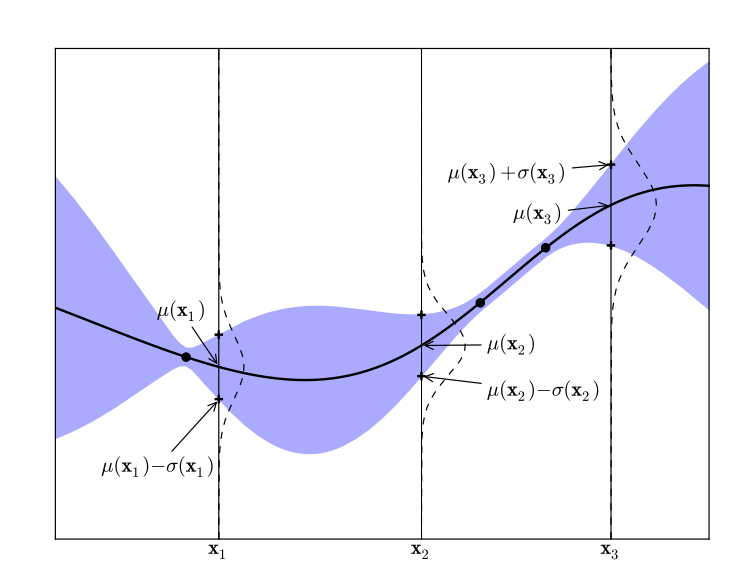
\includegraphics[width=1.0\textwidth]{images/gp-1d.png}
    \caption{A GP regression fit to three data points in 1D, shown as small
    black circles. The black line signifies the mean prediction, while the
    purple filled area shows one standard deviation at each point. The three
    points marked as $x_1, x_2, x_3$ are where we are computing the posterior, that
    is $p(x_1, x_2, x_3 | \mathcal{D})$. These points together have a
    multivariate Gaussian distribution, with a marginal 1D distribution shown
    vertically at each point. In order to draw a plot like this one we compute the
    posterior over a fine grid on the $X$ axis, and plot the mean parameter and the
    diagonal of the covariance matrix, giving us the standard deviation. Image
    source: \cite{nando-bopt-tutorial}.}
		\label{figure:gp-regression-1d}
	\end{center}
\end{figure}

By convention, we assume that the prior mean is a constant zero function, that
is $m(\vx) = 0$. Since the data is often normalized in practice, this does not
reduce the flexibility of the model. The power of a GP comes from its
covariance function, which for any two points $\vx_i$ and $\vx_j$ defines their
covariance $\kappa(\vx_i, \vx_j)$. If $\vx_i$ and $\vx_j$ have a high covariance,
the values of the function at those points will be similar.

\autoref{figure:gp-regression-1d} shows an example of a GP regression in one
dimension. Because GP is a non-parametric model, it uses the whole dataset
$\mathcal{D}$ in order to compute the posterior parameters. A theoretical
benefit of this approach, as compared to using a parametric model like a random
forest, is that we reduce the number of ways our model can underfit or overfit
the data. Because we assume the mean to be zero, our only parameter is the
kernel function $\kappa$. As we will explain later in
\autoref{section:kernels}, we restrict ourselves even further to the Mat\'ern
covariance function, which only has two hyperparameters.

Because the model is non-parametric, it can still fit any arbitrary dataset it
is given, but its flexibility in terms of overfitting is controlled only via
the kernel parameters. As an added benefit we can visualize the change in
kernel parameters over time during Bayesian optimization in order to get
further insight into how the model is fitting the data, as shown in
\autoref{section:kernel-parameter-visualization}.

Intuitively, it is often useful to think of a GP as a function, which instead
of returning a scalar $f(x)$ returns the mean and standard deviation of a
Gaussian distribution over the possible values, centered at $x$. We leave a formal
treatment of GPs until \autoref{chapter:gp}.


\section{Hyperparameter versus Architecture Search}
\label{section:architecture-search}

Using our earlier definition, any parameter which the model does not learn on
its own could be considered a hyperparameter. This definition is broad enough
to allow a lot of flexibility, but some hyperparameters are better for the
framework of Bayesian optimization than others. Discrete and categorical
hyperparameters require special consideration. Bayesian optimization itself is
flexible in the sense that it allows for an arbitrary probabilistic model, but
the specific choice does matter when we consider discrete values. In the case
of GPs, the model itself has the ability to directly work with nothing
but continuous real-valued vectors.

There has been some recent work \citep{integer-valued-gp} showing better
approaches for handling integer-valued variables. The authors suggest to
round the appropriate values before computing their covariance. As the
kernel will consider the values as equivalent, their covariance will be maximized,
and the GP will be forced to predict a constant value over each integer region.
While this approach does help a little bit with integer-valued variables, it
does not improve handling of categorical (nominal) variables, which lack any form of
ordering. If we simply treat them as integers, the GP prior will enforce
relationships which do not exist.

An alternative approach to solving the problem with categorical variables is to
use a different model than GPs, namely random forests
\citep{nando-bayesian-out-of-the-loop}. Their main advantage is the ability to
naturally handle various types of data. We however do not explore random
forests in this work, as many of the hyperparameters of interest when tuning
neural networks are either continuous or integer-valued. Categorical variables,
such as activation functions, are better suited to be tweaked as part of neural
architecture search \citep{nasnet}.

Regardless of the probabilistic model, categorical variables cause many
immediate problems.  Consider the choice between SGD with momentum
\citep{overview-of-sgd} and Adam \citep{kingma2014adam}.  While SGD with
momentum has a \emph{momentum} hyperparameter, Adam does not, but it has its
own two extra hyperparameters, $\beta_1$ and $\beta_2$. This gives us two
different sets of mutually exclusive hyperparameters. Bayesian optimization
however does not have any natural way of handling problems like this. Even if
we did externally enforce two different modes based on which categorical values
was chosen, it would essentially be the same as running two experiments in
parallel, one with SGD, and one with Adam. Another issue arises in
visualization, which is one of the goals of this work. Inspecting the samples
from two or more different modes of the network at once is challenging at best,
and with multiple categorical variables the problem grows exponentially.

For these reasons, we chose not to provide direct support for categorical
variables, apart form converting them to integer variables with ordering and
treating them as such. Some categorical variables can be optimized by simply
treating them as fixed within a particular experiment, and then running
multiple instances of that experiment with a different value each. Other
categorical variables, such as the types of layers, activation functions, or
even the connections between modules, are better left for the framework of
neural architecture search, which treats them in a principled way.


\section{Related work}

There are a few notable mentions of related work in the area of tuning
hyperparameters of neural networks. The main motivation for this work is Google
Vizier \citep{google-vizier}, which is a proprietary service at Google used for
black box optimization. There also exist a few implementations of Bayesian
optimization. Spearmint \citep{spearmint} is the most fully featured one, but
comes with a very restrictive license, and does not perform any visualization
of the results. GPyOpt \citep{gpyopt2016}, RoBO \citep{robo} and
scikit-optimize \citep{scikit-optimize} are the most notable libraries for
Bayesian optimization, but they only provide the basic optimization loop for
Bayesian optimization, and do not handle long running experiments in a possibly
distributed environment.

An important mention is the \cite{automl}, which is an attempt at automating
many aspects of Machine Learning. Several different approaches are being tried,
for example the TPOT \citep{tpot} library uses evolutionary algorithms to not
only tune hyperparameters, but also perform architecture search on Scikit-Learn
algorithms, including building feature pre-processing pipelines, dimensionality
reduction, and feature elimination.

Unfortunately, a commonly shared problem of these higher level approaches is
the explosion of the search space. The more of the ML problem is handed over to
the search procedure, the bigger the search space gets, and at some point one
has to make certain trade-offs. The benefit of libraries as TPOT is their ease
of use on small problems, where the model can be trained within a few minutes.
But as is the goal of this thesis, we are interested in tuning hyperparameters
of models which can take hours or even days to train, and in such case we want
to be as efficient as possible.

Commercial services are also becoming more and more popular, both for AutoML
and just for hyperparameter optimization. Apart from the Google Vizier service
\citep{google-vizier} there also exist others, for example SigOpt
\citep{sigopt} provides a cloud based solution to hyperparameter tuning using
Bayesian optimization. Amazon SageMaker \citep{amazon-sagemaker} is yet another
commercially available cloud based hyperparameter tuning service based on
Bayesian optimization.






\chapter{Gaussian Processes}
\label{chapter:gp}

- uvod, proc to delame
- ucbnicove
- kernely existujou
\\

This chapter goes into the technical details of the Gaussian distribution and
its extension the Gaussian Process (GP). We think it is important to have at
least a basic understanding of the underlying math to make intuitive claims
about the behavior of the model, especially since GPs are a bit different
from other parametric machine learning models.

Since our objective is bayesian optimization, we only derive the properties
necessary for its implementation. Specifically, we are interested in the
conditional and marginal distributions of a multivariate Gaussian. The
conditional Gaussian distribution allows us to compute the posterior $p(f|x)$
at an arbitrary point, and the marginal allows us to fit a GP regression model
to each hyperparameter separately for additional visualization.

Let us now continue with a more rigorous treatment of the Gaussian distribution.
For a more thorough treatment see \cite{bishop2016pattern} and \cite{murphy2012machine}.

\begin{defn}
  A random variable $\rX$ has a \newterm{univariate Gaussian distribution},
  written as $\rX ∼ 𝓝(μ, σ^2)$, when its density is
  $$
    p(x) = \frac{1}{\sqrt{2πσ²}} \exp{\left\{ -\frac{1}{2σ²} (x - μ)² \right\}}.
  $$
  The parameters $μ$ and $σ$ are its \emph{mean} and \emph{standard deviation}.
\end{defn}

\begin{defn}
  % TODO: napsat jinak
  We say $\rX$ has a \newterm{degenerate Gaussian distribution} when $\rX ∼ 𝓝(μ, 0)$.
\end{defn}

% TODO: \mX vs \rX pro vicerozmerne rv
\begin{defn}
  A random variable $\mX \in ℝ^n$ has a \newterm{multivariate Gaussian distribution} if
  any linear combination of its components is a univariate Gaussian, i.e.
  $\va^T \rX = ∑_{i=1}^n \va_i \mX_i$ is a Gaussian for all $\va ∈ ℝ^n$.
  % TODO: tucne μ a Σ
  % TODO: cov sequence?
  We then write $\mX ∼ 𝓝(μ, Σ)$ where $𝔼[\mX_i] = μ_i$
  and $cov(\mX_i, \mX_j) = Σ_{ij}$.
\end{defn}


\begin{rem}
  The parameters $μ$ and $Σ$ uniquely determine the distribution $𝓝(μ, Σ)$.
\end{rem}

\begin{defn}
  A random variable $\mX ∼ 𝓝(μ, Σ)$ has a \newterm{degenerate multivariate Gaussian distribution}
  if $\det Σ = \mZero$.
\end{defn}

\begin{rem}
  Given a random variable $\mX ∼ 𝓝(μ, Σ)$, random variables $\mX_1, \ldots,
  \mX_n$ are independent with distributions $\mX_i ∼ 𝓝(μ_i, σ_i^2)$ if and only
  if $μ = (μ_1, \ldots, μ_n)$ and $Σ = diag(σ₁², \ldots, σₙ²)$.
\end{rem}

\begin{thm}
  If a random variable $\mX ∈ ℝⁿ$ is a multivariate Gaussian, then $\rX_i,
  \rX_j$ are independent if and only if $cov(\rX_i, \rX_j) = 0$. Note that his
  is not true for any random variable, as it is a special property of the
  multivariate Gaussian.
\end{thm}

\begin{proof}
  TODO
\end{proof}

\begin{thm}
  A Gaussian random variable $\rX ∼ 𝓝(\vmu, \mSigma)$ has a density iff
  it is non-degenerate (i.e.\ $\det \mSigma \neq 0$, alternatively $\mSigma$
  is positive-definite). And in this case, the density is

  \begin{equation}
    \label{eq:mvn-definition}
    p(\vx) = \frac{1}{\sqrt{\det(2 π \mSigma)}} \exp{ \left\{ - \frac{1}{2}
    (\vx - \vmu)^T \mSigma^{-1} (\vx - \vmu) \right\} }
  \end{equation}
\end{thm}

\begin{rem}
  The normalizing constant in the denominator is also often in an alternate
  form as $$\det(2 π \mSigma) = (2π)^n \det(\mSigma)$$ which follows from basic
  determinant properties. Alternatively we can also put the square root in the
  exponent $(2 \pi)^{n/2} (\det \mSigma)^{1/2}$.
\end{rem}

\begin{rem}
  A special case of the multivariate gaussian is when $n = 1$, then Note that
  if $n = 1$, then $\mSigma = σ²$, meaning $cov(X, X) = σ²$ , $\mSigma^{-1} =
  \frac{1}{σ²}$, and hence the multivariate Gaussian formula becomes the
  univariate one

  \begin{equation}
    p(x) = \frac{1}{\sqrt{2 π σ²}} \exp{\left\{ - \frac{1}{2σ²} (x - μ)² \right\}}.
  \end{equation}
\end{rem}

\section{Sampling}

Even not of immediate interest for bayesian optimization, we will shortly show
how to generate samples from a multivariate Gaussian, as this can be useful for
visualization purposes with GPs.

\begin{thm}
  Given a random variable $\mX$ with $cov[\mX] = \mSigma$, it follows from
  the definition of covariance that $cov[\mA \mX] = \mA \mSigma \mA^T$.
\end{thm}

\begin{proof}
  \begin{align}
    cov[\mA \mX] &= E[(\mA \mX - E[\mA \mX])(\mA \mX - E[\mA \mX])^T] \\
                 &= E[(\mA \mX - \mA E[\mX])(\mA \mX - \mA E[\mX])^T] \\
                 &= E[\mA (\mX - E[\mX])(\mX - E[\mX])^T \mA^T] \\
                 &= \mA E[(\mX - E[\mX])(\mX - E[\mX])^T] \mA^T \\
                 &= \mA cov[\mX] \mA^T \\
                 &= \mA \Sigma \mA^T
    \label{eq:gaussian-ax}
  \end{align}
\end{proof}

\begin{thm}
  Given a random variable $\mX \sim \gN(\mZero, \mI)$ and a positive-definite matrix
  $\mSigma$ with a cholesky decomposition $\mSigma = \mL \mL^T$, then

  \begin{equation}
    \mL \mX \sim \gN(\mZero, \mSigma).
    \label{eq:gaussian-cholesky}
  \end{equation}
\end{thm}

\begin{proof}
  We can immediately use \eqref{eq:gaussian-ax}.
  \begin{align}
    \mL \mX \sim N(0, \mL \mI \mL^T) = N(0, \mL \mL^T) = N(0, \mSigma)
  \end{align}
\end{proof}

\begin{thm}
  Any affine transformation of a Gaussian is a Gaussian. In particular
  $$
    \rX \sim \gN(\vmu, \mSigma) \implies \mA \rX + \vb \sim \gN(\mA \vmu + \vb, \mA \mSigma \mA^T)
  $$
  for any $\vmu \in \mR^n, \mSigma \in \mR^{n \times n}$ positive
  semi-definite, and any $\mA \in \mR^{m \times n}, \vb \in \mR^m$.
  We call this the \newterm{affine property} of a Gaussian.
\end{thm}

\begin{proof}
  Follows from the linearity of expectation together with \autoref{eq:gaussian-cholesky}.
\end{proof}

Since samples from $\gN(\mZero, \mI)$ can be generated independently, using the
affine property we can generate samples from an arbitrary multivariate
Gaussian. All that is required is a procedure for cholesky decomposition, and a
way of generating independent samples from a univariate gaussian, which can be
achieved using the Box-Muller transform \citep{box-muller1958note}.


\section{Geometric Properties}

If $\mSigma$ is positive-definite, then $\mY \sim \gN(\vmu, \mSigma)$ implies
$\mA^{-1} (\mY - \vmu) ∼ 𝓝(0, \mI)$ where $\mSigma = \mA \mA^T$.  The random
variable $\mA^{-1} (\mY - \vmu)$ has a spherical shape in $n$-dimensional
space.

Looking further at the density formula for a multivariate Gaussian
(\autoref{eq:mvn-definition}) the term $(\vx - \vmu)^T \mSigma^{-1}(\vx -
\vmu)$ is called the Mahalanobis distance between $\vx$ and $\vmu$. If we
consider $\vmu$ a constant, we can also view it as a quadratic form in $x$.
When $\mSigma$ is an identity matrix, the Mahalanobis distance reduces to
Euclidean distance. In general, it can be thought of as a distance on a
hyper-ellipsoid. Let us now derive some intuition for this.

Since $\mSigma$ is a covariance matrix, we know it is positive definite, and we
can perform its eigendecomposition to get $\mSigma = \mU \mLambda \mU^T$, where
$\mU$ is an orthogonal matrix of eigenvectors, and $\mLambda$ is a diagonal
matrix of eigenvalues. Basic matrix algebra gives us
$$
  \mSigma^{-1} = (\mU^T)^{-1} \mLambda^{-1} \mU^{-1} = \mU \mLambda^{-1}
  \mU^T = \sum_{i = 1}^D \frac{1}{\lambda_i} \vu_i \vu_i^T,
$$
where the second to last equality comes from $\mU$ being orthogonal ($\mU^{-1}
= \mU^T$).  Substituting this in the Mahalanobis distance we get
\begin{align}
  (\vx - \vmu)^T \mSigma^{-1} (\vx - \vmu) &= (\vx - \vmu)^T \left( \sum_{i = 1}^D \frac{1}{\lambda_i} \vu_i \vu_i^T \right) (\vx - \vmu) \\
                                           &= \sum_{i = 1}^D (\vx - \vmu)^T \frac{1}{\lambda_i} \vu_i \vu_i^T (\vx - \vmu) \\
                                           &= \sum_{i = 1}^D \frac{y_i^2}{\lambda_i} \label{eq:mvn-ellipse}
\end{align}
where $y_i = u_i^T (\vx - \vmu)$ which has exactly the same form as a $D$
dimensional ellipse. From this we conclude that the contour lines of a
multivariate Guassian will be elliptical, where the eigenvectors determine the
orientation of the ellipse, and the eigenvalues determine the length of the
principal axes \citep{bishop2016pattern}.





\chapter{Bayesian Optimization in depth}

- bopt alg
- jaky kernely v bayes opt., co pouzivame, proc (ref)
- paralelni evaluace
\\

\chapter{Technical Details of Bayesian Optimization}
\label{chapter:bo-indepth}

This chapter provides a more technical insight into Bayesian optimization. We begin by considering acquisition functions from a mathematical perspective, because they form the basis of Bayesian optimization. Next, we show how to extend Bayesian optimization to perform parallel evaluations, work with integer and discrete hyperparameters, and optimize parameters on a logarithmic scale. Finally, we explore the Bayesian optimization algorithm in detail, including some of its numerical properties and issues that can arise when implementing it.

The contents of this chapter deals largely with implementation details and is not necessary to use Bayesian optimization in practice. However, understanding the behavior of integer based hyperparameters, in addition to the overview in \autoref{section:architecture-search}, can prove useful when deciding if a certain hyperparameter makes for a good candidate for automatic tuning using Bayesian optimization.

\section{Acquisition Functions}
\label{section:acq-fn}

An acquisition function is a key component of Bayesian optimization. Together with the GP regression it allows for balancing the exploration-exploitation dilemma in search. The only limitation we impose on the acquisition function is tractability, and possibly continuity, because we need to optimize it. The tractability requirement is mandatory, since without being able to compute the function we could hardly find its maximum. But the continuity requirement is useful given the fact that an acquisition function is often optimized using stochastic gradient optimizers such as L-BFGS.

An intuitive choice for an acquisition function is to maximize the probability
of improving over our currently best achieved value, which is called the
\newterm{probability of improvement}. This can be computed in closed form as
$$
\operatorname{PI}(\vx) = Φ \left( \frac{μ(\vx) - y_{\max}}{σ(\vx)} \right),
$$
where $y_{\max}$ is the maximum value achieved by sampling $f(\vx)$.

A natural extension is the \newterm{expected improvement} (EI) acquisition function,
which is simply the expected improvement over the currently achieved maximum.
We define it as $$\operatorname{EI}(x) = 𝔼[\max(0, f(x) - y_{\max})].$$ At first it might seem that
the expectation would be an intractable integral, but fortunately even this
equation can be computed in closed form as
$$
\operatorname{EI}(x) = Δ(x) + σ(x) φ \left( \frac{Δ(x)}{σ(x)} \right) - |Δ(x)| Φ \left( \frac{Δ(x)}{σ(x)} \right),
$$
where $Δ(x) = μ(x) - y_{\max}$. In practice, the expected improvement shows better results
than the probability of improvement. For more examples of acquisition functions see
\cite{frazier2018tutorial}.

In both of these cases, the next sampling point would be chosen by maximizing
the acquisition function, that is $$x_{\operatorname{next}} = \argmax_x \operatorname{EI}(x)$$ for
the case of expected improvement. This can be performed by utilizing any stochastic optimizer,
such as the commonly chosen L-BFGS with restarts.


\section{Parallel Evaluations}
\label{section:parallel-evaluations}

In practice we might have the means of evaluating $f(\vx)$ at multiple points
in parallel, but the framework we have shown so far only allows for sequential
optimization. A natural extension would be not to optimize with respect
to a single $x_{\operatorname{next}}$, but rather with respect to multiple points. An extension
of EI allowing for optimization with respect to multiple points is called \newterm{parallel expected improvement}.

Unfortunately, maximizing parallel expected improvement has no simple solution \citep{frazier2018tutorial}. A
common solution is the so called \newterm{Constant Liar} approximation, which
chooses $x_{i+1}$ assuming $x_i$ was already chosen, and has the corresponding
value $y_i$ equal to a constant, often chosen to be the expected value of
$f(x_i)$ under the GP posterior.

The Constant Liar approximation enables parallel evaluations by simply
considering the $μ$ prediction for unfinished evaluations as their $y$ value
and consider them part of the dataset $𝓓$.


\section{Integer Hyperparameters}
\label{section:integer-hyperparameters}

GP regression by itself does not have the ability to model integer values in $X$ directly as some other models do (e.g. random forests \autoref{chapter:bo}). A common solution, used by \citep{spearmint} and the one we also adopt in this thesis, is to consider all parameters to be real valued and only round after the GP.

In recently published work \cite{integer-valued-gp} the authors show a more principled approach. The effect of rounding causes the model to consider variation and relationships even inside constant-valued regions. A possible downside is that the model could predict values different enough so that the acquisition function would obtain a maximum within a constant region which was already sampled, thus wasting an evaluation. A proposed solution to this problem is to round the appropriate values right before they are processed by the kernel function, such as
$$\kappa'(x_1, x_2) = \kappa(T(x_1), T(x_2)),$$ where $T(x)$ is an identity for real valued elements and a rounding function for integers.

Our implementation however does not use this approach. Instead, we handle the problem explicitly by detecting the pathological cases, as described in \autoref{chapter:software}.

\section{Logarithmic Scaling of Hyperparameters}

When optimizing hyperparameters we might want to distinguish not only real and integer valued ones, but also their scale. Optimizing the number of training epochs or layers is well modelled by a linear scale, but a learning rate is better modelled using a logarithmic scale.

We adopt a simple solution working independently on Bayesian optimization, by simply transforming all of the appropriate values to logarithmic scale before inputting them into the model, and then transforming them back after we get the next sample proposal $x$. Given this approach is completely transparent from the point of the GP regression model, we could just as well perform an arbitrary bijection.


\section{Implementation Details of Bayesian Optimization}
\label{section:bopt-alg}

We now present the algorithm for Bayesian optimization in greater detail compared to \autoref{alg:bopt}. Let $𝓓_n = \{ (\vx_i, y_i), i \in 1:n\}$ denote a set of $n$ samples (evaluations) of the objective function $f$, with $y_i = f(\vx_i)$. Our goal is to pick the next $\vx_{n+1}$ to maximize our chance of finding the optimum quickly, assuming that already enough points were evaluated for us to fit the GP. \autoref{alg:bopt-detailed} shows one iteration of Bayesian optimization as it proposes $\vx_{n+1}$.

\begin{algorithm}
	\DontPrintSemicolon
	\SetAlgoLined
	Let $\mX$ be the matrix of all $\vx_i$, and $\vy$ be a column vector of all $y_i$. \;
	Maximize the kernel log-likelihood $$p(\mX) = -\frac{1}{2}\vy \mK^{-1}\vy - \frac{1}{2} \log \det \mK - \frac{N}{2} \log (2 π),$$ where $\mK = \kappa(\mX, \mX)$, by tuning the kernel hyperparameters. \;
	Maximize the acquisition function $A(\mX, \vy, \mathcal{G}\mathcal{P})$ as a function of the GP using the kernel hyperparameters obtained in the previous step. \;
	Sample $y_{n+1} = f(\vx)$, where $\vx = \argmax A(\mX, \vy, \mathcal{G}\mathcal{P})$. \;
	Add $y_{n+1}$ to the dataset as $𝓓_{i+1} = 𝓓_i \cup (\vx_{i+1}, y_{i+1})$.
	\caption{Bayesian Optimization with implementation details.}
	\label{alg:bopt-detailed}
\end{algorithm}

While this algorithm explains how Bayesian optimization works, there are a few cases where numerical issues can arise, and we point them out next.

Firstly, the quadratic form $\vy \mK^{-1} \vy$ does not need to be computed using a matrix inversion procedure, which can be numerically unstable and requires more intermediate computation (see \cite{cholesky-inverse-krishnamoorthy2013matrix} for details). In general, consider the equation $\mA \vx = \vb$. We can rewrite it to $\vx = \mA^{-1} \vb$ for an invertible matrix $\mA$. A naive solution would compute the inverse and then the multiplication to get $\inv(\mA) \vb$, but because we do not actually need the inverse itself, we can solve for $\mA^{-1} \vb$ directly using a \inlinecode{solve} procedure \citep{numpy}.

Because the $\mK$ matrix is a covariance matrix, we also know it is positive definite. This allows us to compute its Cholesky factorization $\mL = \chol(\mK)$, and then apply a procedure for \inlinecode{solve} directly on the factorized matrix $\mL$ (in TensorFlow available as \inlinecode{tf.linalg.cholesky\_solve}).

Having just computed the Cholesky factorization we can re-use it in the second expression of the marginal log-likelihood, that is the $\log \det \mK$, since
\begin{align}
\log \det \mK &= \log \det(\mL^T \mL) = \log(\det(\mL^T) \cdot \det(\mL)) = \\
&= 2 \cdot \log \det \mL = 2 \cdot \log \prod \diag \mL = 2 \cdot \sum \log \diag \mL.
\end{align}
This form allows computing the determinant, which usually takes $𝓞(n^3)$, in just linear time, by re-using the work already performed during the Cholesky factorization produced in the previous step.

Another interesting note, discovered by our initial custom implementation, and confirmed in the implementation of the GPy \citep{gpy2014} library, is that when computing a Cholesky factorization of a covariance matrix computed on real world data, it often fails for numerical reasons, and requires additional noise to be added to the diagonal to improve stability. What GPy does internally is to iteratively increase the amount of noise, up until some threshold, to make sure the factorization succeeds, while not adding excessive noise when not needed.

Lastly, the optimization procedures themselves used for maximizing the kernel log-likelihood and acquisition function can be sensitive. Our initial implementation in SciPy and TensorFlow demonstrated quite different results based on the type of the optimizer (SGD, Adam, L-BFGS), and its meta-parameters, such as the number of restarts, stop tolerance criterion, learning rates, etc. These problems, along with many numerical issues encountered along the way, contributed to the choice of using GPy for the final implementation. We outline a few more reasons in \autoref{section:gpy}.


\section{Priors on Kernel Parameters}
\label{section:priors-on-kernel-params}

One of the benefits of the GP regression model is that it is very flexible. Unlike parametric models, such as linear regression, it can fit arbitrarily complex predictions of the data. This flexibility is dictated by the choice of a kernel function, which determines individual covariances between every pair of points. As we have shown earlier (see \autoref{section:kernels}), the kernels themselves have hyperparameters which greatly affect the behavior of the model. Even though it is theoretically possible to set the kernel parameters by hand, as it could be done if we knew some properties of the objective function, we cannot take this approach when fitting arbitrary samples from the loss landscape of a neural network. Instead, we take a principled approach using statistics and optimize the kernel parameters to maximize the likelihood of the data, specifically by using maximum likelihood estimation (MLE).

Unfortunately, because MLE is a point estimate, it is prone to overfitting. In our particular case of using a flexible non-parametric model we can run into severe case of overfitting. In theory, some argue (see \citep{williams2006gaussian}) that when the likelihood function is multi-modal, there are usually multiple interpretations to the data, and each mode maps to an intuitive interpretation. We have not found this to be true on more complex datasets, as those sampled from the objective function of neural networks models, and very often the MLE ends up choosing a model with extremely high capacity, as shown in \autoref{figure:overfitting-gp}.

\begin{figure}
	\begin{center}
		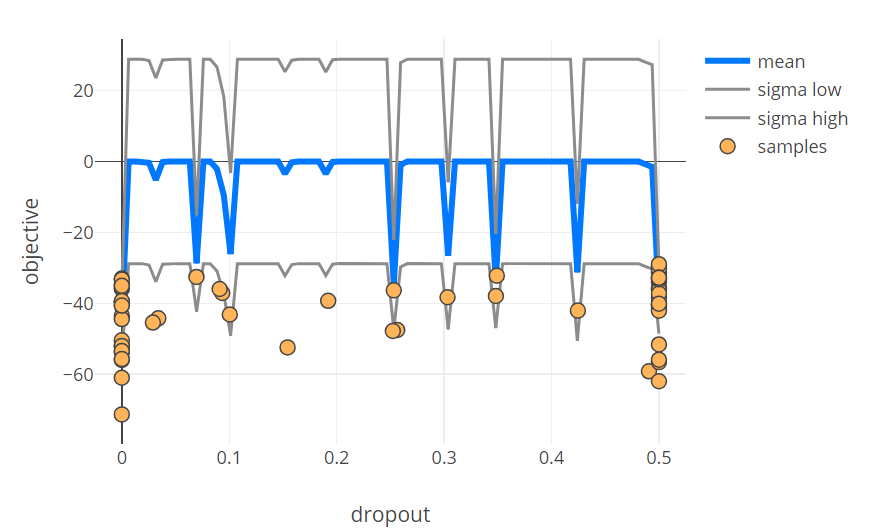
\includegraphics[width=1.0\textwidth]{images/overfitting-gp.png}
		\caption{GP regression with a very low value for the lengthscale kernel parameter. Since the scale parameter is low, the $x$ axis ends up being \emph{stretched out}, and each data point becomes independent, that is their covariance is low. As a result, the model is free to try to fit almost every data point independently on the others, and its predictions become uninformative.}
		\label{figure:overfitting-gp}
	\end{center}
\end{figure}

A common solution to the overfitting problem of MLE is to introduce a prior distribution $p(w)$ on the parameters $w$, and then instead of maximizing the likelihood $p(x|w)$ we would maximize the posterior distribution $p(w | x) \propto p(x | w) p(w)$. This approach is commonly called the maximum a posteriori (MAP) estimate, and is frequently employed in machine learning models as a way of reducing overfitting. For example, in the case of linear regression, the standard least squares solution corresponds to maximizing the likelihood of the data using MLE, or equivalently minimizing the mean squared error between the predictions and the labels. A probabilistic extension of linear regression, which introduces a Gaussian prior on the weights, is called a Ridge regression (or L2 regularization), and corresponds to computing the MAP estimate of the parameters, or equivalently minimizing the mean squared error with an additional weight decay term.

In the ideal case, we would either marginalize over the parameters, or take a fully Bayesian approach and compute the posterior $p(w | x)$. Unfortunately, in many cases including ours, the marginalization becomes intractable due to the normalization constant given by the evidence term $p(x)$. The MAP estimate is a practical compromise between the frequentist point estimate using MLE, and a fully Bayesian treatment. Because we only need to compute the $\argmax$ of the posterior, we can optimize it without computing the normalization term $p(x)$, given $\argmax$ being invariant to scaling by a constant. The MAP estimate is then simply computed as $$ \argmax_w p(x|w) p(w), $$ where in our case $w$ represents the kernel parameters, as well as the constant for Gaussian noise in each sample.

As with any Bayesian method, the choice of a prior is of great importance. If we were to choose a uniform prior, computing the MAP estimate would be equivalent to computing the MLE with constrained optimization on the support of the uniform distribution. In practice, we could take a conservative step and choose a non-informative prior, which would still act as regularization, and possibly help with overfitting as compared to computing a bare MLE estimate. An example of such prior is the $\operatorname{Gamma}(1.0, 0.001)$ distribution shown in \autoref{figure:gamma-prior}, because its support are positive real numbers, and both the variance and the lengthscale of the kernel are also defined only for positive real numbers.

In our experiments described in \autoref{chapter:experiments}, we show a few cases where the choice of an uninformative prior leads to poor model behavior. The common cause if the model choosing a small lengthscale for hyperparameters with high range of values, as shown previously in \autoref{figure:overfitting-gp}. Because the process of Bayesian optimization is built on top of the regression model, it can become problematic when the model considers most of the search space as constant regions with only a few peaks at the sampled data points.

A possible solution to this problem is to abandon the idea of non-informative priors and instead adopt the approach often called Empirical Bayes \citep{murphy2012machine}, where the parameters of the prior distribution are estimated from the data themselves. Choosing between a non-informative prior and estimating the parameters from data is a principal problem that does not have a definitive answer.

With our motivations being largely driven by practical applications rather than theoretical purity, we do estimate the prior parameters from data in some visualizations (see \autoref{section:visualizations}) to avoid pathological cases and provide more useful user experience. We also show comparisons between the non-informative priors and the Empirical Bayes approach in the GP regression model used when computing the acquisition function, as compared to only in visualizations, in \autoref{section:experiments-empirical-bayes}. Unfortunately, because some experiments were very computationally intensive (some over a thousand GPU-hours), we do not provide a full ablation analysis.

\begin{figure}
	\begin{center}
		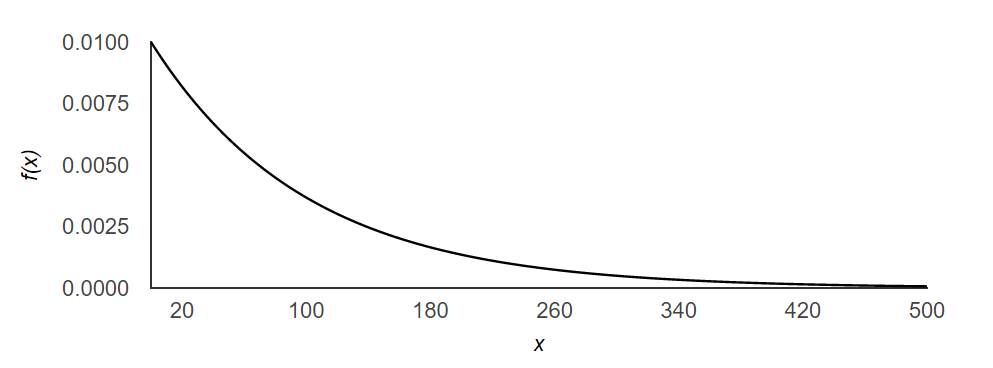
\includegraphics[width=1.0\textwidth]{images/gamma-prior.png}
		\caption{An example of a prior distribution defined as $\operatorname{Gamma}(1.0, 0.001)$ with support over positive real numbers.}
		\label{figure:gamma-prior}
	\end{center}
\end{figure}




\chapter{Software}

- co umime
- vizualizace
- jak se to pousti, runnery, serializace
\\

\chapter{Software}
\label{chapter:software}

This chapter describes the implementation part of this thesis. While we do not provide any theoretical extensions to Bayesian optimization, we instead provide a modular and fully working implementation which was tested on multiple experiments. The implementation is provided as a Python (\cite{python}) package called \bopt (short for Bayesian optimization).

The main features of the package are:

\begin{itemize}
	\item A robust implementation of Bayesian optimization.
    \item Flexible experiment configuration with random search and GP backends.
    \item Parallel execution of evaluations, both on the local machine and on a cluster.
    \item Robust error handling with duplicate/similar sample detection.
    \item Command line interface for controlling the experiment evaluations, including running a manual evaluation with user specified hyperparameters.
    \item Simple filesystem based storage with user-readable and editable serialization format based on YAML.
    \item Web based visualizations of the whole optimization process, including
    1D and 2D slices and marginal plots at all points during the evaluation.
    \item Ability to add manual samples either from another, already executed, experiment. Or simply by running the appropriate command with user-provided hyperparameter values.
\end{itemize}


\section{Architecture}

In this section we will explore the high level architecture of \bopt. Everything is structured around a central class \inlinecode{Experiment}, which represents a single objective function together with a configuration of its hyperparameters, and configuration for the Bayesian optimization itself. The \inlinecode{Experiment} can contain multiple \inlinecode{Samples}, where each sample represents a single evaluation of the objective function.

We assume the function being optimized can be evaluated by running a script file. The hyperparameters will be passed as command line arguments (see \autoref{section:command-line-interface}), and the output will be parsed from the standard output using a regular expression provided by the user. This provides the user with maximum flexibility with regards how the actual function is being executed, as \bopt will simply spawn the process, pass the command line arguments, and then wait for it to terminate to collect the output and parse the result. If the result is not found in the output, or the process exists with an exit code greater than $0$ it will mark the evaluation as failed. We do not put any restrictions on the type of script the user might want to provide. It is solely at the discretion of the \inlinecode{Runner} (see \autoref{section:runners}) to figure out how to run the provided file.

Each \bopt experiment is located in its own directory on the filesystem (called the \newterm{\inlinecode{meta\_dir}}), where it stores all of the information in a single \inlinecode{meta.yml} file, along with output files for each job. This makes it easy for the user to manually inspect and edit if needed, or even backup when performing more complicated operations, such as deleting specific samples, or manually adding samples from a different experiment. Since Bayesian optimization is memory-less, that is always starting from scratch, the user can easily combine evaluations from multiple different experiments by hand, or even delete samples which were created by accident, such as when using manual evaluations.


\subsection{Samples, Result Collection and Locking}

Each evaluation of the objective function is split into two parts. One being the \inlinecode{Sample}, which contains the specific hyperparameter values for $x$, kernel parameters of the GP model which was used to compute the sample, a posterior prediction of its mean and variance, and then the second part, which is an optional \inlinecode{Job} instance, which represents the actual running evaluation. The \inlinecode{Job} simply wraps the running process 

Each \inlinecode{Sample} can also have an optional \inlinecode{Job}, which only wraps the process ID with runner-specific information on how to get the status of the running job, kill it, etc. The \inlinecode{Sample} only represents a snapshot at one point in time. Every time a \bopt command is executed, or whenever a new state is required, a \emph{result collection procedure} will be called, which checks the status of all running jobs, and updates their respective samples with any results or failure information. This is done mainly to avoid race conditions, as the evaluations themselves are running asynchronously from the main program flow in \bopt. Apart from the collection procedure and a few exceptions, such as starting a new job, the main data structure is considered read only.

It is also worth mentioning, that since multiple instances of \bopt could be running at any given time, we have employed a file locking mechanism which creates a \inlinecode{.lockfile} file in the experiment directory, which any other \bopt instance would detect and wait on release. This allows the user to use the command line utilities while an experiment is running without worrying about data corruption.

\subsection{Runners}
\label{section:runners}

Training neural networks is a computationally intensive task, and tuning hyperparameters makes it an order of magnitude more expensive. As a result, running some experiment on a local computer might not be an option for the user. The package was designed with different evaluation environments in mind and provides a flexible concept of a \inlinecode{Runner} class, which abstracts away the process of starting a new evaluation, that is figuring out how and where to run the script file representing the objective function.

We provide two different runners out of the box:

\begin{description}
    \item[Local] runs the process on the same machine as \bopt.
    \item[SGE] submits a job to the Son of Grid Engine \citep{sge}.
\end{description}

All runners support job parallelism using the Constant Liar approximation (see \autoref{section:parallel-evaluations}), which is part of the reason why each \inlinecode{Sample} stores a mean prediction. This value is being used as $y$ whenever a new evaluation point needs to be chosen during parallel evaluations.

When a job is started, its stdout and stderr will be redirected to a file within an \inlinecode{output} directory in the \inlinecode{meta\_dir}. The file will be named with a process ID (PID) in case of a \emph{local} job, and with a job ID in case of an \emph{SGE} job. In case of the local runner we have to employ a minor trick, because when \inlinecode{popen} is being called with stdout redirection it already requires a file handle, but at that time the process ID is unknown. We work around this by creating a temporary file, redirecting the output to that, and then after \inlinecode{popen} returns a PID we rename the opened temporary file to a new name with the PID. Since UNIX systems can handle renaming of open files this workaround causes no issues, but the behavior on Microsoft Windows is unclear. If the user needs to support Microsoft Windows they might have to provide their own runner which does not use PIDs, but rather generates the ID based on some other process which makes the ID available before the child process is spawned. The SGE runner does not run into this issue, because we only specify the filename as a parameter to \inlinecode{qsub}, which then handles the process scheduling, creation, redirection, and names the output file accordingly.

To implement a custom runner, the user only needs to subclass two classes, namely the \inlinecode{Job} and the \inlinecode{Runner}. The \inlinecode{Job} class needs to mainly implement an \inlinecode{is\_finished} method (among a few other ones described in the abstract interface), which simply returns the status of the evaluation based on the implementation details specified in the runner. To implement the \inlinecode{Runner} the user needs to provide a \inlinecode{start} method, which accepts the values of all hyperparameters, and returns a new \inlinecode{Job}, which will later be evaluated. An additional requirement is that the \inlinecode{Job} needs to store its result in an appropriately named file, specifically \inlinecode{job.oID} in the \inlinecode{outputs} directory. This was done mainly to avoid some issues with process IDs as described earlier in this section.

Lastly, it is worth mentioning that \bopt supports the UNIX \inlinecode{time} command for measuring the runtime of an evaluation. Because we allow running jobs on an SGE cluster we can not simply take the start time and end time and subtract them to get the total run time, because the job can sit in a queue for an arbitrary amount of time.

\section{GPy}
\label{section:gpy}

Our library of choice for GP regression is the \cite{gpy2014} library, as it is the most stable and robust package available, and is still being actively developed. We're mainly interested in the \inlinecode{GPy.models.GPRegression} class which implements the regression model itself, and the \inlinecode{GPy.kern} module, which implements the kernel functions. We initially used our own custom implementation of GP regression (partly shown in \autoref{section:bopt-alg}) in TensorFlow \citep{tensorflow2015-whitepaper} and SciPy \citep{scipy}, but despite the seemingly short and simple numeric algorithm for computing the regression, getting all the details right proved to be an exceedingly difficult task. Even simple numerical methods like Cholesky decomposition are often wrapped with layers of numerical stability tricks that one does not get out of the box with libraries like NumPy \citep{numpy}.

For these reasons we ended up switching to the GPy library, which apart from a numerically stable implementation provides many additional benefits. Being built upon a general purpose parameter optimization library \cite{paramz}, GPy allows the user to both put arbitrary constraints on each of the parameters, as well a specify a prior distribution which is then used when optimizing the kernel marginal likelihood.

\section{Random Search}

The core optimization loop has the ability to generate samples randomly, which is useful for two reasons. It allows us to create a comparative baseline where all samples are generated using random search, so that we can measure the benefits and improvement of Bayesian optimization. But it also serves as a way of bootstrapping the Bayesian optimization driven search. When choosing an initial first point of evaluation, we don't have any data to fit the model to. We could optimize the acquisition function on the prior, but since our prior has zero mean, it would simply be a uniform distribution. What we do instead is sample each hyperparameter randomly, until we have enough points to fit the probabilistic model.

The number of random samples can increase if we are using parallel evaluations, simply because if we need to start $N$ jobs at the same time, with no prior data, we have no way of even calculating a mean prediction. As a result, we always start the first $N$ evaluations using random search.

\section{Command Line Interface}
\label{section:command-line-interface}

Since larger experiments will most likely always be run on a compute cluster we opted for a command line interface which can be easily used over an SSH connection, and is very flexible. The available subcommands of \bopt are:

\begin{description}
    \item[init] Creates a new experiment with a given script, configuration of hyperparameters and runner options.
    \item[exp] Prints out the current status of a given experiment, showing metadata on all the evaluations.
    \item[web] Starts the web interface for visualizing the evaluations.
    \item[run] Starts a run loop which tracks how many jobs are currently running, starting new as needed to fulfill the parallelism requirements, and collects the results as needed.
    \item[run-single] Runs a single evaluation, regardless of how many are currently running.
    \item[manual-run] Runs a single evaluation with hyperparameters provided by the user. This does not use Bayesian optimization and simply serves as an interface to manually start tasks as needed.
    \item[suggest] Prints a suggestion for the next evaluation without running it, as well as an already formatted command for \inlinecode{manual-run} so that the user can inspect the hyperparameter values and run the command immediately if they see fit.
    \item[debug] Starts a Python debugger with the given experiment loaded in, which can be useful both for diagnosing issues as well as exploring the internal data structures.
    \item[clean] Kills all running jobs and removes all evaluations from the experiment, while keeping the initialization metadata. This command is basically just a shortcut for re-starting an experiment from scratch.
\end{description}

All commands are executed as \inlinecode{bopt COMMAND} and support the conventional \inlinecode{--help} command line arugment, which prints out all of the available options, as well as their descriptions.

\subsection{Meta Directory, Data Corruption and \inlinecode{-C}}
\label{section:meta-dir}

When an experiment is initialized all of its information will be stored in its own directory. This includes both the meta information about hyperparameters, run configurations and evaluations, as well as the job outputs themselves.

The \bopt command was designed such that it will always try to acquire an exclusive lock on the directory using a \inlinecode{.lockfile}, which is to prevent any race conditions and possible data corruption from running multiple instances of \bopt at the same time. Such scenario could easily occur when the user would run a long running \inlinecode{bopt run} command, while also exploring the results, and possibly starting a few more evaluations manually using \inlinecode{bopt run-single}, \inlinecode{bopt manual-run}, or even another \inlinecode{bopt run}. Because of the locking behavior, it is completely safe to run as many instances of \bopt as are needed, and the user does not need to concern themselves with causing any data corruption via the command line interface. We also make sure to always serialize the data into a new file, and then atomically move over the existing one, in order to minimize possible data corruption when the \bopt process is killed.

It is important to note that \bopt was designed with manual user intervention in mind. As such, the \inlinecode{meta.yml} file, which contains all of the experiment information, was created to be easily human editable. But because \bopt does not use the UNIX \inlinecode{flock} mechanism (as editors do not obey it), the user has to be wary of editing the file by hand while other instances of \bopt are running. Because the \inlinecode{meta.yml} file is overwritten atomically, the user can even edit the file while \bopt is running, but they have to make sure to save at the appropriate time, e.g. not to discard the changes that were just written after the file was loaded in the editor. This problem is unlikely to occur in editors like Vim, which will notify the user of the file being changed after it was read, but it is still does not prevent the user to overwrite it. If there are no existing \bopt processes running, it is completely safe to alter the \inlinecode{meta.yml} file.

All of the \bopt commands will also accept a \inlinecode{-C} command line argument, which specifies a directory to \inlinecode{cd} into before any of the main code is executed (similarly as a \inlinecode{Makefile} would behave). This behavior allows \bopt to always assume it is being executed from within the \inlinecode{meta\_dir} and simplify many possible problems with storing paths in the config files. While this behavior is unlikely to affect the user in a negative way, it is still useful to know the semantics of the program.

We now explore two of the most important commands in more detail, \inlinecode{bopt init} and \inlinecode{bopt run}.

\subsection{\inlinecode{bopt init}}

Initializing experiments is an important feature and as such the command line interface has been streamlined to allow the user to input the arguments without complicated config files. An example of a common \inlinecode{bopt init} call could look something like the following:

\begin{center}
\begin{verbatim}
bopt init \
  --param "batch_size:int:4:128" \
  --param "gamma:logscale_float:0.5:1.0" \
  --param "lr:logscale_float:1e-6:1e-1" \
  --param "dropout:float:0.1:0.6"
  -C experiments/reinforce \
  --runner sge \
  --ard=1 --gamma-prior=1 \
  --gamma-a=1.0 --gamma-b=0.001 \
  $PWD/reinforce.sh
\end{verbatim}	
\end{center}


Let us now go over the arguments one by one. The first four arguments specify four different hyperaparameters, namely batch\_size, gamma, lr and dropout, each with a different type and range. The general format is \inlinecode{NAME:TYPE:MIN:MAX} where \inlinecode{NAME} can be an arbitrary name, \inlinecode{TYPE} can be one of \inlinecode{int}, \inlinecode{float}, \inlinecode{logscale\_int}, \inlinecode{logscale\_float}, and \inlinecode{discrete}, and \inlinecode{MIN:MAX} are simply the bounds of the hyperparameter. If the type of \inlinecode{discrete} is specified, instead of providing the bounds the user would provide a colon separated list of possible values, which would then be encoded as ordinal integers. An example of such discrete hyperparameter could be an activation function defined as \inlinecode{activation:discrete:tanh:relu:sigmoid}. However, as mentioned in \autoref{section:architecture-search}, we do not recommend using \bopt for architecture search, which discourages from most uses of the \inlinecode{discrete} type.

The next argument \inlinecode{-C experiments/reinforce} simply defines the \inlinecode{meta\_dir} where the experiment data will be stored. Next we define the runner type, which can be one of \inlinecode{local} and \inlinecode{sge}.

After the runner is defined, we configure the GP regression itself, in this case by specifying the \inlinecode{ard} flag on, which uses a separate lengthscale parameter for each component of $x$ (more details can be found in the \cite{gpy} documentation). Next we specify that we want to use a Gamma prior on the hyperaparameters, and its shape and scale parameters. A complete list of all flags for configuring the GP regression, acquisition function, kernel and the optimizer can be found using the help flag as \inlinecode{bopt init --help}.

Lastly, we provide \bopt with the script to run, in this case it is \inlinecode{reinforce.sh}, which encapsulates our objective function. We also specify it as an absolute path using the \inlinecode{PWD} environment variable, but this is shown mainly as an interesting trick that can be useful if the \inlinecode{PATH} is not configured in the environment where the runner will execute the job.

After the command exists, it will create a directory \inlinecode{experiments/reinforce} with a \inlinecode{meta.yml} file inside. The following listing shows the contents of the file

\begin{center}
\begin{verbatim}
gp_config: !!python/object:bopt.gp_config.GPConfig
  acq_n_restarts: 25
  acq_xi: 0.001
  acquisition_fn: ei
  ard: true
  gamma_a: 1.0
  gamma_b: 0.001
  gamma_prior: true
  kernel: Mat52
  num_optimize_restarts: 10
  random_search_only: false
hyperparameters:
  batch_size:
    high: 128
    low: 4
    type: int
  gamma:
    high: 1.0
    low: 0.5
    type: logscale_float
  hidden_layer:
    high: 128
    low: 2
    type: int
  learning_rate:
    high: 0.1
    low: 1.0e-06
    type: logscale_float
result_regex: RESULT=(.*)
runner:
  arguments: []
  manual_arg_fnames: []
  qsub_arguments: []
  runner_type: sge_runner
  script_path: ./reinforce.sh
samples: []
\end{verbatim}
\end{center}

Apart from the command line arguments we have provided it should be noted that a few unspecified values were filled in with the defaults. For example, the kernel function was chosen to be the default Mat\'ern $5/2$ kernel, which was shown \citep{snoek2012practical} to perform the best on many hyperparameter tuning tasks. We have tried to make the optimization procedure as configurable as possible in case the user has any additional prior knowledge which might help them optimize better.

In general, there are no significant requirements on the script, as we execute it as a subprocess. We only require that it takes the hyperparameter values as command line arguments in the format of \inlinecode{--NAME=VALUE}, and outputs the objective function on its standard output. By default, we will parse the standard output with a regex \inlinecode{RESULT=(.*)}, but the user is free to modify this in the \inlinecode{meta.yml} file however they see fit. If the user wishes to run an existing software which does not accept command line arguments in this form, they have to wrap the program in a script which will pre-process the arguments given by \bopt, and pass them through in the format they require. This approach allows for maximum flexibility without having to spend large amounts of effort on building a general argument passing system. In our experiments with existing software we only found a few cases where minor argument processing was necessary.

\subsection{\inlinecode{bopt run}}

After the experiment was initialized the user can start running evaluations. Since everything is already configured in the \inlinecode{meta.yml} file the user simply needs to run \inlinecode{bopt run -C experiments/reinforce}, or \inlinecode{cd} into the directory and just run \inlinecode{bopt run}. Both of these variants are equivalent.

By default, this would run $20$ evaluations in total with no parallelism. The number of evaluations can be controlled with the \inlinecode{--n\_iter} switch, while the number of jobs running in parallel is controlled by the \inlinecode{--n\_parallel} switch.

The way \inlinecode{bopt run} tracks the number of running jobs is by checking the \inlinecode{meta.yml} file for the IDs, and then checking the job status and counting how many are running. This allows it to respect the number of jobs running prior to the execution of \inlinecode{bopt run}. If the user first was to start say $5$ evaluations by hand (e.g. using \inlinecode{bopt run-single}) and only then run \inlinecode{bopt run --n\_parallel=5} while the first $5$ jobs were still running, the instance of \inlinecode{bopt run} would correctly identify the running jobs and wait for some of them to finish before launching new ones.

\section{Visualizations}
\label{section:visualizations}

Given the complex nature of tuning hyperparameters, one might be tempted to simply run grid search and examine the results. Ignoring the computational aspects for a moment, let us focus on the manual inspection of the results. As the number of hyperparameters grows beyond to $5$ -- $10$ it becomes very difficult to infer relationships between hyperparameters from a flat list of evaluations. \autoref{figure:sample-table} shows an example of a table with $6$ different hyperparameters. To model a $6$-dimensional space one needs to run at least $15$ -- $20$ evaluations to get enough information to infer relationships between the dimensions. But as the number of evaluations grow, it becomes increasingly difficult to look at tabular data and infer relationships from them.

\begin{figure}
	\begin{center}
		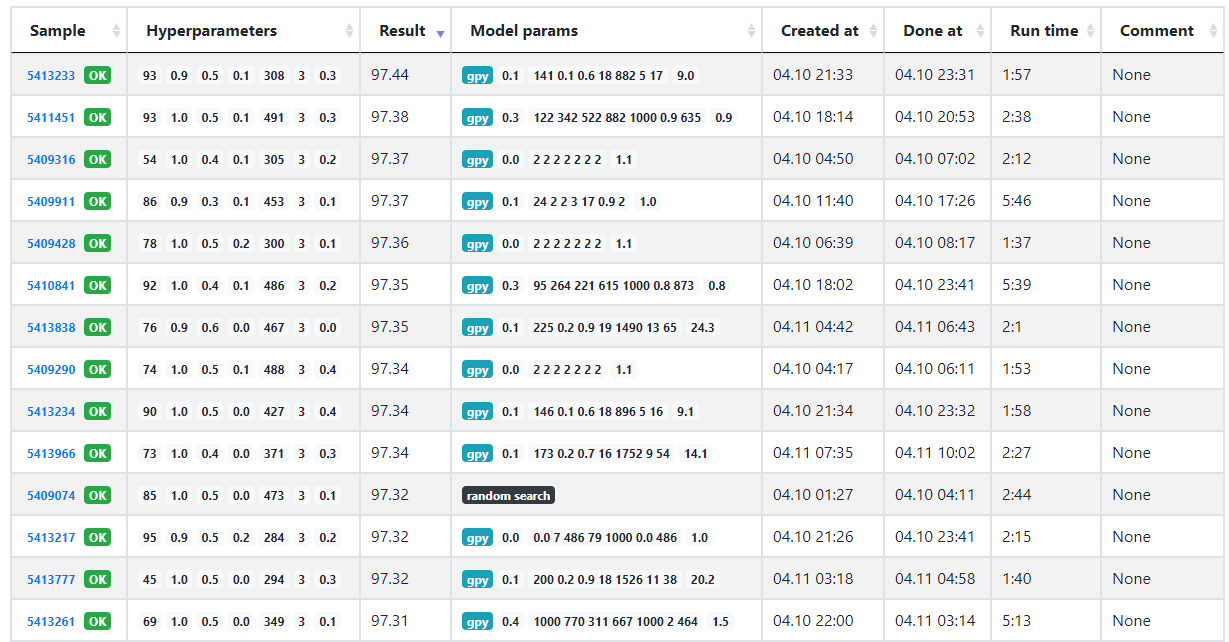
\includegraphics[width=1.0\textwidth]{images/sample-table.png}
		\caption{A table showing the results of multiple objective function evaluations.}
	\end{center}
\end{figure}
\label{figure:sample-table}

We provide a practical solution of plotting 1D and 2D marginal GP fits for all hyperparameters and their combinations. In \autoref{figure:2d-marginal} we show the relationship between two of the hyperparameters as measured in one of our experiments (more details in \autoref{chapter:experiments}). We can also show each 1D marginal in order to visualize how each hyperparameter affects the fitness irrespective of the others, as shown in \autoref{figure:1d-marginal}. The 1D figures can also plot the acquisition function, which can also serve as a useful debugging tool, e.g. to diagnose possible overfitting of the GP. Lastly, we also allow the user to view these visualizations at any point in time during the optimization process, as shown in \autoref{figure:timeline-view}. This allows to view the GP regression as more evaluations were created.

\begin{figure}
	\begin{center}
		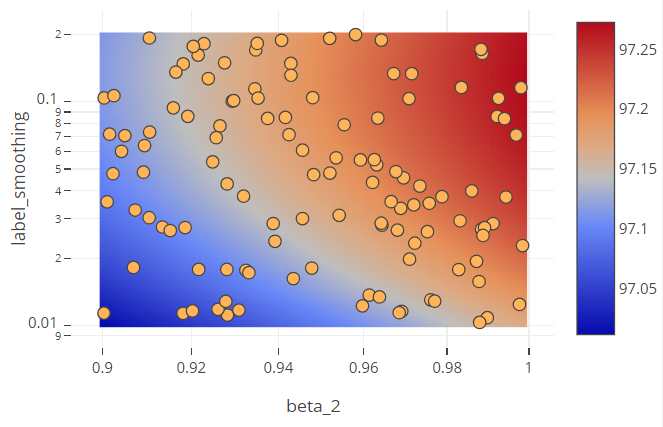
\includegraphics[width=1.0\textwidth]{images/2d-marginal.png}
		\caption{2D marginal plot showing the dependence between $\beta_2$ and \emph{label smoothing} in one of our experiments when training a larger tagger and lemmatizer network on a Czech treebank.}
	\end{center}
\end{figure}
\label{figure:2d-marginal}

\begin{figure}
	\begin{center}
		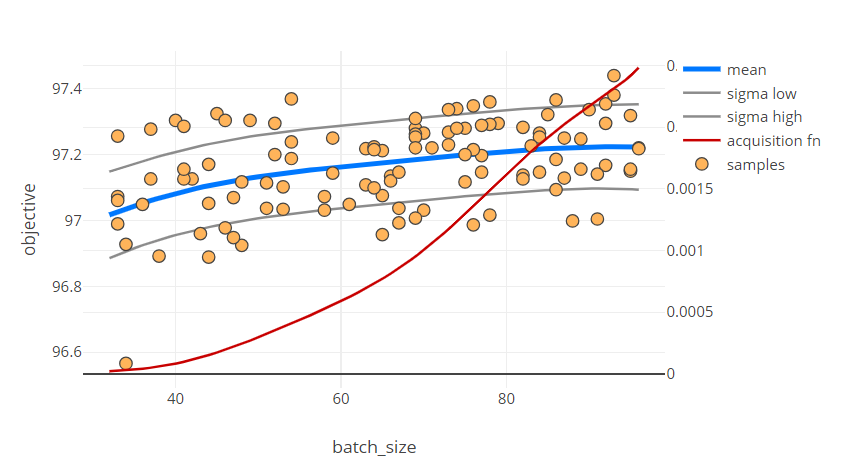
\includegraphics[width=1.0\textwidth]{images/1d-marginal.png}
		\caption{1D marginal plot showing the effect of \emph{batch size} on the objective function on the same model as shown in \autoref{figure:2d-marginal}. The red line shows the value of the acquisition function.}
	\end{center}
\end{figure}
\label{figure:1d-marginal}

The benefit of a GP regression model is that the marginal distribution on any combination if the hyperparameters simply follows the marginalization property (see \autoref{eq:mvn-marginal-parameters}), which says we can only look at the mean and covariance of the parameters we are interested in, as all of the other ones get marginalized out, that is $p(\vx_2) \sim \mathcal{N}(\vx_2 | \vmu_2, \mSigma_{22})$ where $p(\vx_2) = \int p(\vx_1, \vx_2)\ d\vx_1$ and a partitioned matrix $\mSigma$ as described in \autoref{chapter:gp}. Using this property, we can compute the 1D marginal projection by fitting a model to the coordinate corresponding to the hyperparameter of interest. As the goal of the marginal plots is to quickly see the trends in the data, we employ the Empirical Bayes approach described in \autoref{section:priors-on-kernel-params} to bias the prior distribution on kernel parameters towards smoother kernel functions, to avoid pathological cases of overfitting as shown in \autoref{figure:overfitting-gp}.

Similarly, we might be interested in looking at slices through the GP regression model, that is fixing a value of some hyperparameters, and examining how the objective changes when interpolating through the remaining ones. This is again simple to achieve computationally when the model is a GP, because by slicing we are simply conditioning on the values of some elements of $\vx$ while leaving the others free. Using the conditioning formula shown in \autoref{eq:mvn-conditional-parameters} we can compute the posterior parameters in closed form, and then simply plot the predicted mean and variance. We don't show this case in the figures since the plots look exactly the same as the marginal ones, except of course for the specific values. The user can simply toggle between the two modes.

The kernel parameters for the conditioned GP are set to the exact values computed when the sample was chosen for evaluation. This way we can explore the progress of the optimization process through time and see what the model saw at each point, and why it chose the hyperparameters it did.

\begin{figure}
	\begin{center}
		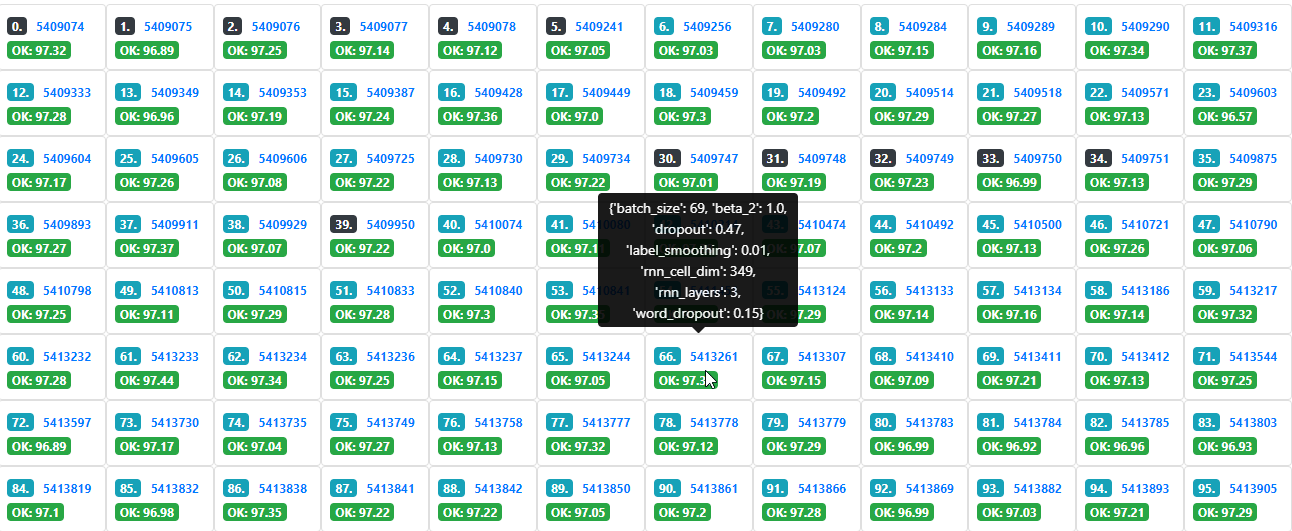
\includegraphics[width=1.0\textwidth]{images/timeline-view.png}
		\caption{A timeline showing all of the evaluated experiments, together with their objective value, model type (shown in color), and the hyperparameters used for evaluation. The user can select any of the evaluations on the timeline and all of the plots will be shown from the perspective of that evaluation, i.e. what the model \emph{saw} when choosing the hyperparameters of that specific evaluation.}
		\label{figure:timeline-view}
	\end{center}
\end{figure}


\subsection{Kernel Parameter Visualization}
\label{section:kernel-parameter-visualization}

\begin{figure}
	\begin{center}
		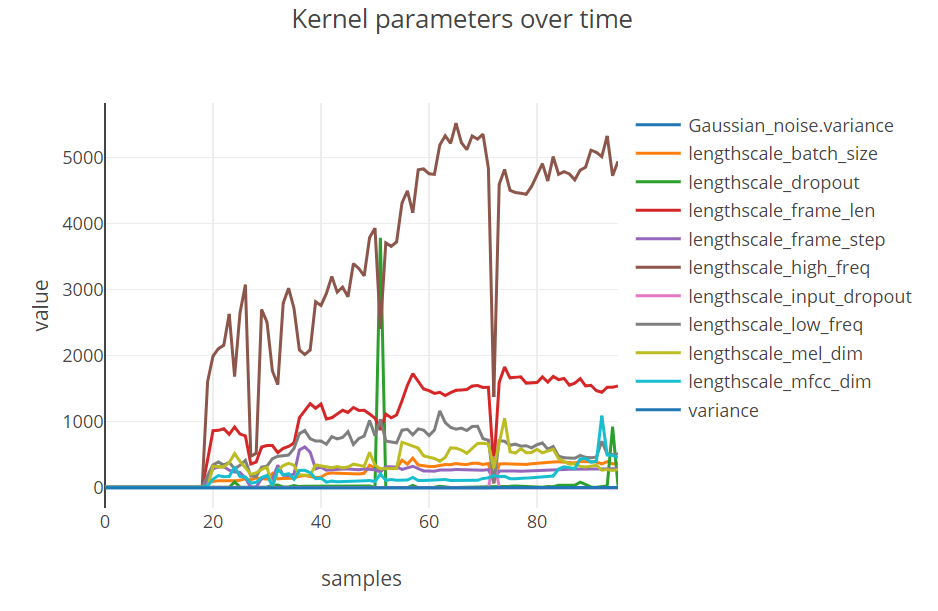
\includegraphics[width=1.0\textwidth]{images/kernel-params-over-time.png}
		\caption{Visualization of the kernel parameters over time as the Bayesian optimization progresses. In this case the model was allowed one lengthscale $\mathcal{l}$ parameter for each element of $x$, in essence allowing it to normalize each column independently. Since there are $9$ different hyperparameters the search space is $9$-dimensional, and as a result it takes the model up to $20$ samples to find a good fit in the data. After that, it automatically determines the scale of each parameter, such as the \emph{high\_freq} parameter, which was optimized on the scale of $1000$ -- $8000$. We can see the model clearly adapting its lengthscale to a similar range. As a general rule of thumb, when the lengthscale parameter is on the same order as the hyperparameter range, the model will scale that parameter to roughly unit range.}
		\label{figure:kernel-parameters-over-time}
	\end{center}
\end{figure}

\begin{figure}
	\begin{center}
		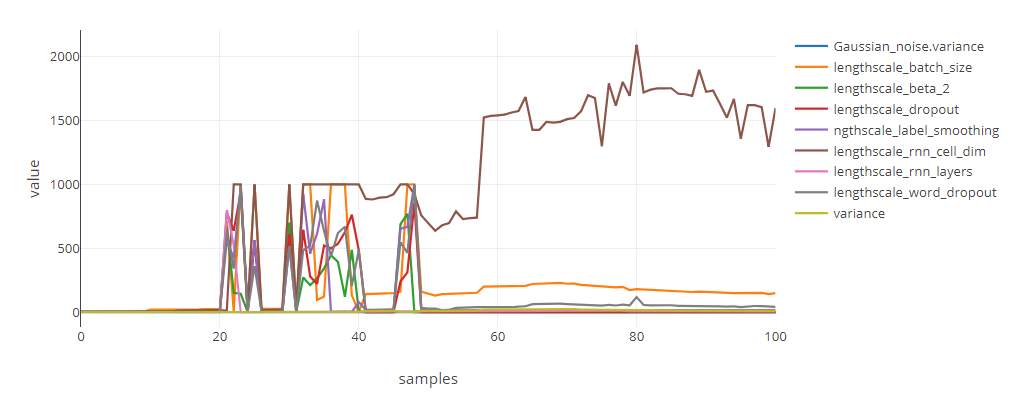
\includegraphics[width=1.0\textwidth]{images/kernel-parameters-over-time-jumpy.png}
		\caption{Visualization of a less stable model with kernel parameters rapidly changing until around 50 samples are evaluated. In this case we attribute the instability to a very noisy objective function, where the model took a long time to fit the right value of variance to counteract the effect of the noise.}
		\label{figure:kernel-parameters-over-time-jumpy}
	\end{center}
\end{figure}

As a method of debugging possible issues in the model, as well as just general high level inspection of the quality of the fit, we provide a visualization of the kernel parameters as they change over time of the Bayesian optimization, as shown in \autoref{figure:kernel-parameters-over-time}.

The kernel hyperparameters roughly determine the general properties of the regression curve and confidence intervals. A large lengthscale results in smooth functions, while small lengthscale results in many spikes without larger continuous regions. Plotting the value of each kernel parameter as the optimization progresses allows us to judge how much does the regression model's view of the objective function change over time.

Intuitively, after we have sampled enough data points, we would expect that adding one additional sample would have an effect on the regression curve itself, but not as much on its quality, such as smoothness. A large change in the kernel parameters signifies that it now sees the objective function completely differently than what it saw before. We would expect the parameters to change over time as the model refines itself to more data, but there should be a visible trend. In \autoref{figure:kernel-parameters-over-time} we show an example where for most of the samples the kernel parameters don't change by much, but there are two visible drops (around 45 and 55) in the \emph{high\_freq} lengthscale, which signify a possible issue in the GP regression at that point. Based on our experience with the model, we would still consider the example to be quite stable, as compared to another example shown in \autoref{figure:kernel-parameters-over-time-jumpy}, where until around 50 samples the model was not sure how to scale individual hyperparameters, and only stabilized afterwards. In this case we attribute the problem to a much noisier model.

\subsection{Convergence}
\label{section:convergence}

Looking at the results in a table does not always explain how well is the Bayesian optimization process doing. We add a convergence plot, which shows both the intermediate values of the objective, as well as a cumulative maximum. 

In some cases the model might be achieving steady increase in the objective, as shown in \autoref{figure:convergence-plot}, while in others it might fail to improve in a significant way. The following \autoref{chapter:experiments} shows experiments where even though the model showed some improvement over the baseline, it clearly did not converge as more evaluations were computed, which becomes clearly visible in its convergence plot as shown in \autoref{figure:convergence-plot-long-exp}.

\begin{figure}
	\begin{center}
		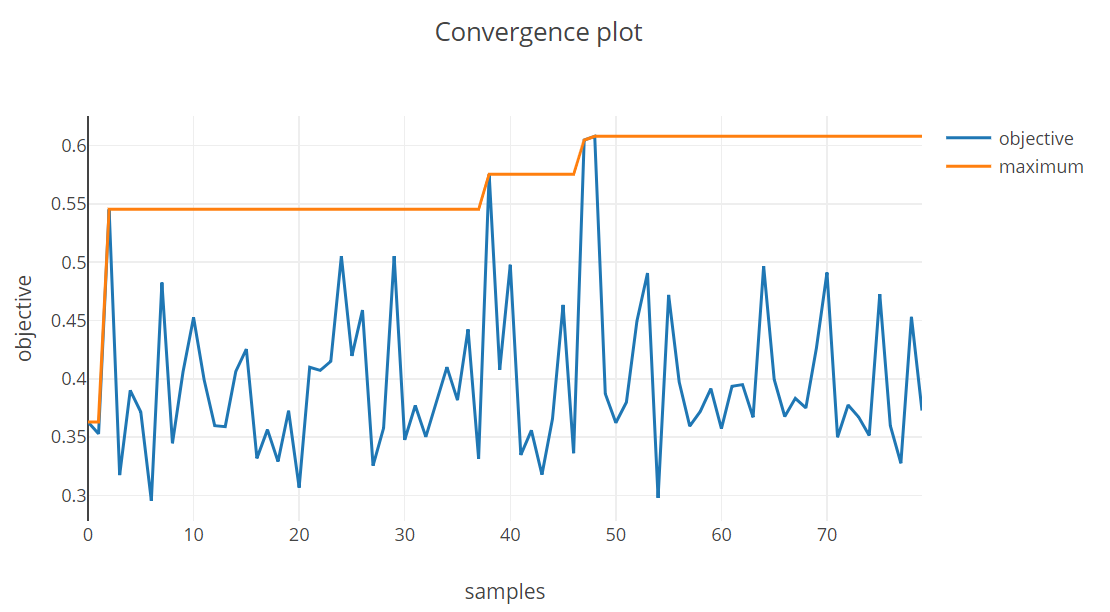
\includegraphics[width=1.0\textwidth]{images/convergence-plot.png}
		\caption{Visualization of the overall convergence of the optimization process. The $x$ axis labels time as new samples of are evaluated, and $y$ axis labels the objective function. We show both the intermediate results (blue), as well as the cumulative maximum (orange).}
	\end{center}
\end{figure}
\label{figure:convergence-plot}

\begin{figure}
	\begin{center}
		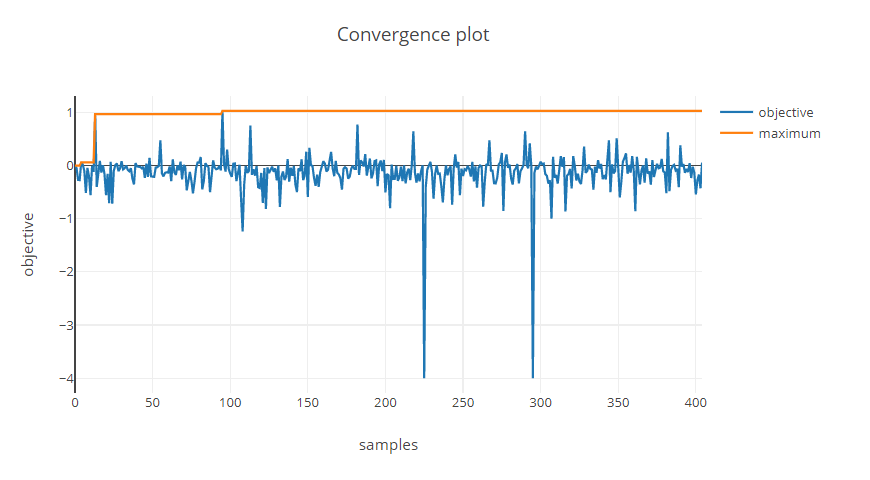
\includegraphics[width=1.0\textwidth]{images/convergence-plot-long-exp.png}
		\caption{Convergence plot of a long running experiment where no significant improvement over the baseline is found. In this particular case the objective was measured as an improvement over an existing model.}
	\end{center}
\end{figure}
\label{figure:convergence-plot-long-exp}


\section{Inspecting Attached Experiments}

We provide results for some of the experiments as an attachment to this work. Because of the design described in \autoref{section:meta-dir} we only need to store the \inlinecode{meta.yml} file after the results have been collected, as the collection copies all of the results in.

Inspecting the results is then simply a matter of running either \inlinecode{bopt web -C dir} for the web interface, or \inlinecode{bopt exp -C dir} for the command line inspector, where \inlinecode{dir} is a directory containing the \inlinecode{meta.yml} file.




\chapter{Experiments}

- toy tasky
  - porovnani existujici fuj fce na optimalizaci
  - srovnani acq/kernel, random search (ze to neco dela)

- maly ulohy

- velka uloha

- interpretace vysledku
\\

\chapter{Experiments}
\label{chapter:experiments}

This chapter goes over some of the experiments we have conducted to evaluate the viability of Bayesian optimization. All of the cases are examples of optimizing neural networks, as that is the area of interest of this work.

We present one example from reinforcement learning, specifically the REINFORCE algorithm \citep{suttonbarto2018reinforcement}, as an example of a smaller and simpler network. This case also compares Bayesian optimization with random search. Next we show a larger experiment where we train a recurrent neural network (RNN, \cite{dlbook}), specifically a tagger, on a SIGMORPHON 2019 shared task \citep{sigmorphon2019task2}, where the network is trained on a significantly larger dataset. Lastly, we show two smaller examples, one of a tokenizer written in C++, and second a network for speech recognition.

\section{REINFORCE}

TODO: lower variance than random search?

\subsection{Comparing Priors on Kernel Parameters}
\label{section:experiments-empirical-bayes}

In this section we show the effect of setting kernel prior parameters from the data based on a simple heuristic.

TODO: empirical bayes


\section{Tuning on Multiple Treebanks Simultaneously}
\label{section:multiple-treebanks-failed}

\begin{figure}
	\begin{center}
		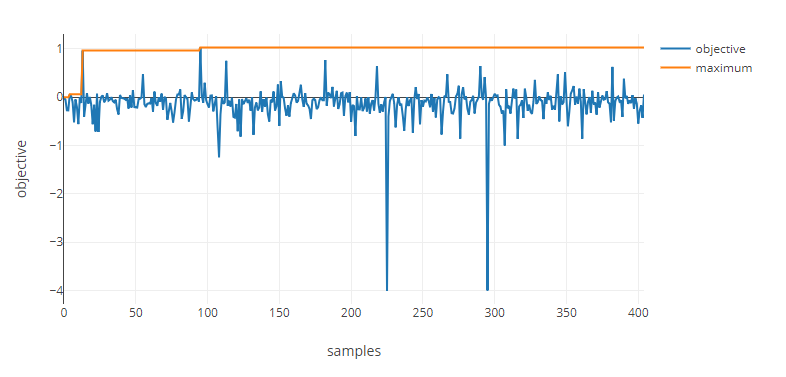
\includegraphics[width=1.0\textwidth]{images/sigmorphon-convergence.png}
		\caption{Convergence plot for a model trained on the SIGMORPHON 2019 shared task. No significant improvement over the baseline was found.}
		\label{figure:sigmorphon-convergence}
	\end{center}
\end{figure}

\begin{figure}
	\begin{center}
		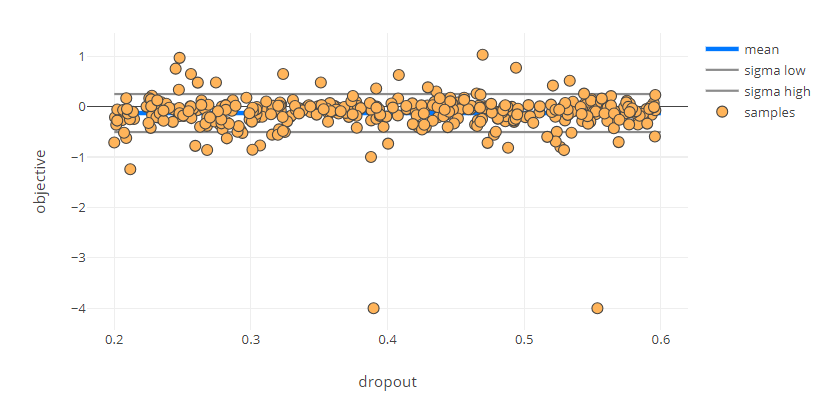
\includegraphics[width=1.0\textwidth]{images/sigmorphon-dropout.png}
		\caption{Marginal regression on the dropout hyperparameter for the SIGMORPHON 2019 shared task when training on all 105 treebanks.}
		\label{figure:sigmorphon-dropout}
	\end{center}
\end{figure}

In this larger experiment we tried to tune hyperparameters for a single model on multiple different datasets at once. Specifically, the model was trained on for the SIGMORPHON 2019 shared task 2 \citep{sigmorphon2019task2} on 105 different treebanks, most of which are different languages. Our goal was to ideally find one set of hyperparameters that would work well across all of these treebanks. Even though this experiment was not ultimately successful we still include it in the text as the problem being solved poses interesting technical challenges from the perspective of hyperparameter tuning.

As a fundamental problem of this task, each treebank is of different size, and the difficulty of different languages varies a lot. To give a few specific examples, on Tamil the model achieves around 95\% accuracy in tagging, while on Sanskrit it achieves only 65\%. This makes it nearly impossible to set the objective function to simply be the accuracy of the model, as the same value of hyperparameters could result in the objective varying by 30\%. 

We work around this problem by computing a baseline accuracy using an existing, hand tuned, model on the same task, pre-computing its score for each treebank with a fixed set of hyperparameters, and then subtracting its value from the accuracy of our tuned model. The objective function then explicitly becomes the improvement over an existing fixed model.

A second problem we had to solve was how to incorporate the 105 treebanks into the optimization procedure. Because training the model takes multiple GPU hours even for the smaller treebanks we realistically cannot perform more than a few hundred evaluations total. Instead of training the model on all treebanks for each set of hyperparameters we only train the model on one treebank for each hyperparameter configuration chosen by Bayesian optimization.

This introduces an interesting choice. In theory, we could treat the treebank as a hyperparameter treated explicitly by Bayesian optimization. As the algorithm balances the exploration-exploitation tradeoff it should be able to pick treebanks as needed to better explore the space. But because of the different sizes and difficulties of each treebank, and the inability of Bayesian optimization to treat categorical hyperparameters well, we decided to not take this approach.

Instead, we omit the treebank from the list of hyperparameters so that the optimizer has no way of modeling it, and provide it as an explicit parameter outside of the scope of the optimizer. In theory, we could also provide the optimizer with a treebank that was used with each valuation and not allow it to optimize it when choosing a next point by overriding its choice, but this approach would most likely yield sub-optimal choices by the optimizer, as the samples would be chosen based on a different criteria than what the optimizer sees. Instead, our way of completely removing the treebank parameter from the optimization process will be seen by the optimizer as noise on the output. If it were to evaluate the same hyperparameters multiple times, the evaluation itself would receive a different treebank, and the improvement over the baseline would be different. In effect this captures our desire to find a set of hyperparameters that works well across all treebanks.

Unfortunately, our experimental results did not find a significant improvement over the hyperparameters found by hand-tuning the network (see \autoref{figure:sigmorphon-convergence}). One of the reasons is that the size of the treebank affects which hyperparameter combinations result in value of the objective function. An example of using tuning the same model on a larger treebank is shown in \autoref{section:exp-cestina}.

To give a specific example, when the \emph{batch\_size} hyperparameter is set to a larger value, it will work well on a larger treebank, but the opposite is true for a smaller treebank, where a smaller \emph{batch\_size} acts as a regularizer. This means our samples at the same batch size will be spread as far as is the objective on all treebanks. Unfortunately, this spread ends up being so large that all of the hyperparameter end up having no visible trend, as no value is clearly better than the others, as shown in \autoref{figure:sigmorphon-dropout}.


\section{Tagger on a Single Treebank}
\label{section:exp-cestina}


\begin{figure}
	\begin{center}
		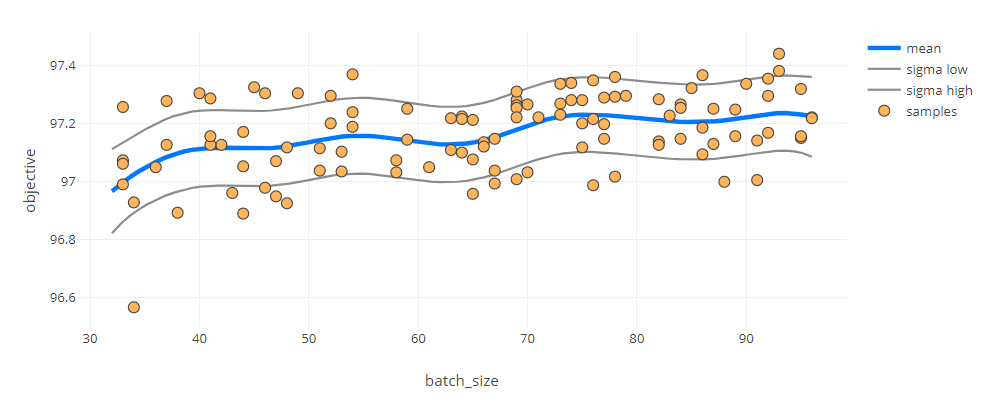
\includegraphics[width=1.0\textwidth]{images/czech-batch-size.png}
		\caption{Marginal regression on the \emph{batch\_size} hyperparameter for the SIGMORPHON 2019 shared task when training on a single Czech treebank.}
		\label{figure:czech-batch-size}
	\end{center}
\end{figure}


\begin{figure}
	\begin{center}
		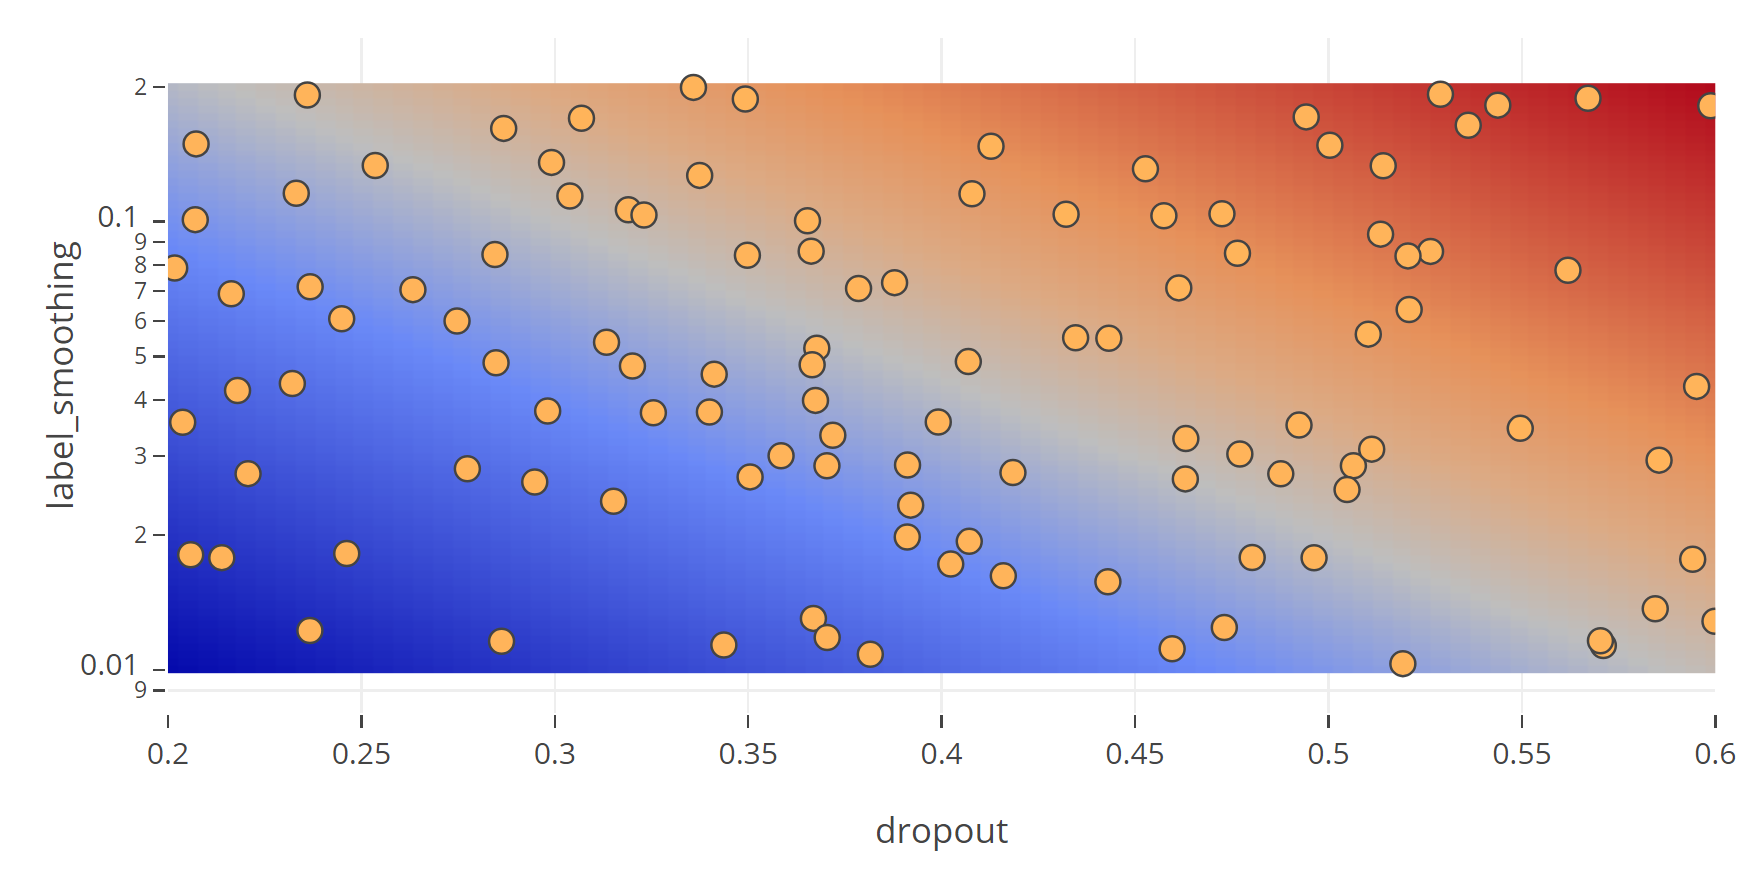
\includegraphics[width=1.0\textwidth]{images/czech-2d-marginal.png}
		\caption{Marginal regression on the \emph{label\_smoothing} and \emph{dropout} hyperparameters for the SIGMORPHON 2019 shared task when training on a single Czech treebank. A correlation between the two parameters is clearly visible, showing that setting only one of them to the correct value is not enough to achieve a high value of the objective function.}
		\label{figure:czech-2d-marginal}
	\end{center}
\end{figure}

Contrary to the experiment shown in \autoref{section:multiple-treebanks-failed} in this experiment we train the same model but only on a single treebank at a time. We tried two different treebanks, Czech and English, which are both larger. We chose the larger treebanks because they provide a more consistent evaluation metric, as the smaller ones are many orders of magnitude smaller, and pose a greater risk of overfitting even on the validation set.

While the previous experiment (see \autoref{section:multiple-treebanks-failed}) did not find any trends in the hyperparameters, the one we present here did find a clear trend in most, as shown for example in \autoref{figure:czech-batch-size}, where larger \emph{batch\_size} is better. In some cases we also found clear relationships between two hyperparameters, such as in the case of \emph{label\_smoothing} and \emph{dropout} shown in \autoref{figure:czech-2d-marginal}


\section{Other Smaller Experiments}

In this section we briefly show some interesting results from our last two experiments. First, let us show the experiment where we optimized hyperparameters of UDPipe \citep{udpipe:2017} on tokenization of Czech, English and Ancient Greek.

\begin{figure}
	\begin{center}
		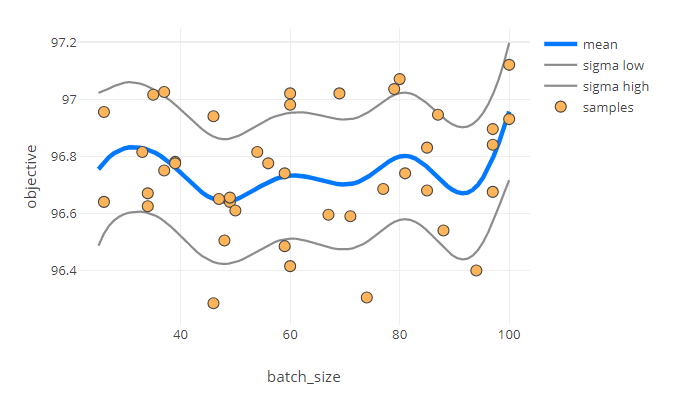
\includegraphics[width=1.0\textwidth]{images/gp-overfitting-batch-size.png}
		\caption{GP regression overfitting on the marginal distribution of \emph{batch\_size}.}
		\label{figure:gp-overfitting-batch-size}
	\end{center}
\end{figure}

Some of the interesting result in this case are the failure cases of the GP regression, particularly how it can overfit on seemingly uninformative dataset, as shown in \autoref{figure:gp-overfitting-batch-size}. These examples nicely show the high capacity of a GP which, even when we set informative priors, is able to find a surprising way to fit the data with high likelihood. Despite these problems, the Bayesian optimization approach still managed to find hyperparameter values with an objective very close to that find by an exhaustive grid search. Because of the acquisition function, even if the model overfits and picks a bad sample, it will be able to correct itself right afterwards, as the area that was previously receiving high value of acquisition function was explored.

As a result, the model still might end up wasting computation time by evaluating incorrect areas by overfitting on the data, but we have not observed it to get stuck in a local optima. Because Bayesian optimization explicitly models exploration into its decision making it quite often ends up doing a decent job of exploring most of the search space, as is visible in all of the figures.



- maly ulohy

- velka uloha

- interpretace vysledku
\\


\chapter{Conclusion}

- future work

- pribalit vysledky experimentu a jak jednoduse pustit web




- parser
- tokenizer/segmentace
- speech recognition
- opennmt lemmatizace
- $reinforce_with_baseline$





---

Let $𝓓_n = \{ (\symbf{x}_i, y_i), i \in 1:n\}$ denote a set of $n$ samples
(evaluations) of the function $f$, that is $y_i = f(\symbf{x}_i)$. Our goal is
to pick the next $\symbf{x}_{n+1}$ to maximize our chance of finding the
optimum quickly.

Consider the set of all continuous functions $f ∈ 𝓕$ with a prior distribution
$p(f)$.  Conditioning on our samples gives us a posterior distribution over
possible functions $p(f | 𝓓)$.

---



% \chapter{Basic Definitions}

\section{Information Theory}

The basic intuition behind information theory is that learning that an unlikely event has occurred is more informative than learning that a likely event has occurred \citep{Goodfellow-et-al-2016}. We define \newterm{self-information} of a random event $x$ as

\begin{equation}
I(x) = -\log P(x).
\end{equation}

The overall information in a probability distribution is quantified by \newterm{Shanon entropy}:

\begin{equation}
H(X) = \E_{X \sim P} [ I(X) ] = -\E_{X \sim P} [ log P(x) ]
\end{equation}

We can extend this to the case of a continuous random variable with a probability density function $f$, in which case we call $H(f)$ the \newterm{differential entropy} and define it as

\begin{equation}
H(f) = - \int_X f(x) log f(x) \dx
\end{equation}

\section{Calculus of Variations}

Before we can derive the Gaussian distribution, we first introduce a few concepts from the calculus of variations.

A \newterm{functional} is a mapping which assigns real numbers to each function belonging to some class \citep{gelfand2012calculus}. We can say that a functional is a special kind of function, where the argument is itself a function. In our case the functional will be the differential entropy $H(f)$. Similarly to derivatives and partial derivatives in real analysis, we can take \newterm{functional derivatives} of a functional $H(f)$ with respect

As full derivation of functional derivatives is outside the scope of this thesis, we only present the following theorem without proof, and refer the reader to the above cited textbook for a proof \todo{find the proof}.

For differentiable functions $f(\vx)$ and $g(y, \vx)$ with continuous derivatives, the following holds

\begin{equation}
\frac{\delta}{\delta f(\vx)} \int g(f(\vx), \vx) d \vx = \frac{\partial}{\partial y} g(f(\vx), \vx).
\end{equation}

\todo{rewrite, copied over from DLB} To gain some intuition for this identity, one can think of $f(\vx)$ as being a vector with uncountably many elements, indexed by a real vector $\vx$. In this (somewhat incomplete) view, the identity providing the functional derivatives is the same as what we would obtain for a vector $\vtheta \in \sR^n$ indexed by positive integers:

\begin{equation}
\frac{\partial}{\partial \theta_i} \sum_j g(\theta_j, j) = \frac{\partial}{\partial \theta_i} g(\theta_i, i).
\end{equation}

\section{Maximum Entropy Probability Distribution}

In this section we derive the Gaussian distribution as a distribution which maximizes differential entropy when the mean and variance are fixed. Similarly as we would optimize a function by computing its gradient, setting it to zero and solving the equation, we can optimize a functional by solving for a function where the variational derivative is zero at every point.

Because we want our resulting functional to be a probability distribution, we need its density to integrate to $1$, specifically

\begin{equation}
\int f(x) \dx = 1
\end{equation}

We also want the mean and variance to be fixed constants $\mu$ and $\sigma^2$ respectively. This gives us the following

\begin{align}
\int x f(x) \dx = \mu \\
\int (x - \mu) ^2 f(x) \dx = \sigma^2
\end{align}

We can solve for all of these constraints simultaneously using Lagrange multipliers. The Lagrangian has the following form:

\begin{align}
\begin{split}
\gL[f] ={}& H[f] + \lambda_1 \left( \int f(x) \dx - 1 \right) + \lambda_2 \left( \int x f(x) \dx - \mu \right) + \\
 &+ \lambda_3 \left( \int (x - \mu)^2 f(x) \dx - \sigma^2 \right)
\end{split} \\
%
\begin{split}
={}& -\int f(x) \log f(x) \dx  + \lambda_1 \left( \int f(x) \dx - 1 \right) + \\
&+ \lambda_2 \left( \int x p(x) \dx - \mu \right) + \lambda_3 \left( \int (x - \mu)^2  f(x) \dx - \sigma^2 \right)
\end{split} \\
%
\begin{split}
={}& \int ( - f(x) \log f(x) + \lambda_1 f(x) - \lambda_1 + \\
&+ \lambda_2 x p(x) - \lambda_2 \mu + \lambda_3 (x - \mu)^2  f(x) - \lambda_3 \sigma^2 ) \dx \\
\end{split} \\
%
\begin{split}
={}& \int ( - f(x)\log f(x) + \lambda_1 f(x) + \lambda_2 x f(x) + \lambda_3 (x - \mu)^2  f(x) ) \dx + \\
&- \lambda_1 - \lambda_2 \mu - \lambda_3 \sigma^2 \label{eq:gauss-lagrangian}
\end{split}
\end{align}

\todo{check the functional derivative, so far only copied from DLB, fix alignment of = in 1.11} We set the following functional derivative of \eqref{eq:gauss-lagrangian} equal to $0$:

\begin{equation}
\forall x, \frac{\delta}{\delta f(x)} \gL = \lambda_1 + \lambda_2 x + \lambda_3 (x - \mu)^2 - 1 - \log f(x) = 0.
\end{equation}

Now simply solving for $f(x)$ we obtain:

\begin{equation}
f(x) = \exp \left( \lambda_1 + \lambda_2 x + \lambda_3 (x - \mu)^2 - 1 \right).
\end{equation}

\todo{rewrite, mostly written as in DLB}
To solve the optimization problem we can choose any value for the $\lambda$. We set $\lambda_1 = 1 - \log \sigma \sqrt{2 \pi}$, $\lambda_2 = 0$, and $\lambda_3 = - \frac{1}{2 \sigma^2}$ to obtain the density of a Gaussian distribution

\begin{equation}
f(x) = \gN(x | \mu, \sigma^2).
\end{equation}

This derivation is one of the reason why a Gaussian distribution is so useful. \todo{rewrite, copied from DLB} Because the normal distribution has the maximum entropy, we impose the least possible amount of structure by making this assumption.


% \chapter{Gaussian distribution}


\section{Univariate Gaussian distribution}

\begin{defn}
    Random variable $X$ has a \newterm{Univariate Gaussian distribution}, written as $\rX \sim \gN(\mu, \sigma^2), \mu \in \sR, \sigma^2 > 0$, which means $X$ has a density
    
    \begin{equation}
        f(x) = \frac{1}{\sqrt{2 \pi \sigma^2}} \exp{ \left\{ -\frac{1}{2\sigma^2} (x - \mu)^2 \right\}}.
    \end{equation}
\end{defn}

\begin{defn}
    \newterm{Degenerate Univariate Gaussian} is:
    
    \begin{equation}
        \rX \sim \gN(\mu, 0)
    \end{equation}
    
    if $\rX \equiv \mu$ (i.e.\ $X(\omega) = \mu, \forall \omega \in \Omega$)
\end{defn}

\begin{defn}
    {TODO co to vubec znamena "has a density"?}
    
    A random variable $\rX \in \sR^n$ is a \newterm{multivariate Gaussian} if any linear combination of its components is univariate Gaussian, i.e. $\va^T \mX = \sum_{i=1}^n \va_i \mX_i$ is Gaussian ($\forall \va \in \mR^n$).
\end{defn}

\begin{defn}
    $\rX \sim \gN(\vmu, \mSigma)$ means $X$ is a Gaussian with $E[\rX_i] = \vmu_i$, and $cov(\rX_i, \rX_j) = \mSigma_{ij}$. Note that this implies that $\mSigma$ is positive semi-definite.
\end{defn}

\begin{rem}
    Note that $\vmu$ and $\mSigma$ uniquely determine the distribution $\gN(\vmu, \mSigma)$
\end{rem}

\begin{defn}
    $\rX \sim \gN(\vmu, \mSigma)$ is \newterm{degenerate multivariate Gaussian}, if $\det \mSigma = \mZero$.
\end{defn}

\begin{rem}
    $\rX_1, \dots, \rX_n$ are independent with $\rX_i \sim \gN(\mu_i, \sigma_i^2)$ iff $\rX = (\rX_1, \dots, \rX_n) \sim \gN(\vmu, \mSigma)$, where $\vmu = (\mu_1, \dots, \mu_n)$ and $\mSigma = diag(\sigma_1^2, \dots, \sigma_n^2)$
\end{rem}

\begin{thm}
    If $\rX \in \mR^n$ is Gaussian, then $\rX_i, \rX_j$ are independent iff $cov(\rX_i, \rX_j) = 0$. Note this is not true in general, and is a special property of the Gaussian.
\end{thm}

\begin{thm}
    $\rX_1, \dots, \rX_n$ each univariate Gaussian \emph{does not imply} $\rX = (\rX_1, \dots, \rX_n)$ is a multivariate Gaussian.
\end{thm}

\begin{thm}
    A Gaussian random variable $\rX \sim \gN(\vmu, \mSigma)$ has a density iff it is non-degenerate (i.e.\ $\det \mSigma \neq 0$, alternatively $\mSigma$ is positive-definite).
    
    And in this case,
    
    \begin{equation}
        f(\vx) = \frac{1}{\sqrt{\det(2 \pi \mSigma)}} \exp{ \left\{ - \frac{1}{2} (\vx - \vmu)^T \mSigma^{-1} (\vx - \vmu) \right\} }
    \end{equation}
    
    Note that $\det(2 \pi \mSigma) = (2\pi)^n \det(\mSigma)$. Alternatively $(2 \pi)^{n/2} (\det \mSigma)^{1/2}$ {TODO check and proof}. Also note that $\det \mSigma \neq$ implies that $\mSigma$ is invertible, which conincides with the density requiring an invertible $\mSigma$.
    
    Also note that if $n = 1$, then $\mSigma = \sigma^2$, $cov(X, X) = \sigma^2 x$, $\mSigma^{-1} = \frac{1}{\sigma^2}$, and hence the multivariate Gaussian formula becomes the univariate one.
    
    \begin{equation}
        \frac{1}{\sqrt{2 \pi \sigma^2}} \exp{\left\{ - \frac{1}{2} \frac{1}{\sigma^2} (x - \mu)^2\right\}}
    \end{equation}
\end{thm}

\begin{defn}
    The \newterm{moment generating function} of a random variable $X$ is
    
    \begin{equation}
    M_X(t) = \E[e^{t X}].
    \end{equation}
\end{defn}

We state the following result without proof {TODO citace, pridat proof}.

\begin{thm}
    Let $X$ and $Y$ be two random variables. If
    
    \begin{equation}
    M_X(t) = M_Y(t)
    \end{equation}
    
    for all $t \in (-\delta, \delta)$ for some $\delta > 0$, then $X$ and $Y$ have the same distribution. We'll use this theorem to show that the sum of Gaussian random variables has a Gaussian distribution.
\end{thm}

\begin{thm}
    \citep{mitzenmacher2017probability}\label{thm:sum-independent-gaussian}
    If $X$ and $Y$ are independent random variables, then
    
    \begin{equation}
    M_{X + Y}(t) = M_X(t) M_Y(t)
    \end{equation}
    
    \begin{proof}
        \begin{equation}
        M_{X + Y}(t) = \E[e^{t(X + Y)}] = \E[e^{tX} e^{tY}] = \E[e^{tX}] \E[e^{tY}] = M_X(t) M_Y(t)
        \end{equation}
        
        Here we have used that $X$ and $Y$ are independent -- and hence $e^{tX}$ and $e^{tY}$ are independent -- to conclude that $\E[e^{tX} e^{tY}] = \E[e^{tX}] \E[e^{tY}]$. {TODO prepsat? prakticky opsano}
    \end{proof}
\end{thm}


\begin{thm}
    Moment generating function of a Gaussian distribution is
    
    \begin{equation}
        M_X(t) = e^{t \mu + \frac{1}{2}\sigma^2 t^2}.
    \end{equation}
\end{thm}

\begin{thm}
    Let $X$ and $Y$ be independent random variables with distributions $\gN(\mu_1, \sigma_1^2)$ and $\gN(\mu_2, \sigma_2^2)$, respectively. Then $X + Y$ is distributed according to the normal distribution $\gN(\mu_1 + \mu_2, \sigma_1^2 + \sigma_2^2)$.
    
    \begin{proof}
    The moment generating function of a sum of independent random variables is the product of their moment generating functions (Theorem \ref{thm:sum-independent-gaussian}). Thus,
    
    \begin{equation}
    M_{X + Y}(t) = M_X(t) M_Y(t) = e^{t^2 \sigma_1^2 / 2 + \mu_1 t} e^{t^2 \sigma_2^2 / 2 + \mu_2 t} = e^{t^2 (\sigma_1^2 + \sigma_1^2) / 2 + (\mu_1 + \mu_2) t}
    \end{equation}
    
    The rightmost expression is the moment generating function of a normal distribution. Theorem \ref{thm:sum-independent-gaussian} implies that $X + Y$ has a normal distribution with the corresponding parameters. {TODO opsano z \citep{mitzenmacher2017probability}}
    \end{proof}
\end{thm}

\begin{thm}
    If random vectors $\mX, \mY \in \sR^n$ where $\mX \sim \gN(\vmu_x, \mSigma_x)$ and $\mY \sim \gN(\vmu_y, \mSigma_y)$ are independent, then
    
    \begin{equation}
        \mX + \mY \sim \gN(\vmu_x + \vmu_y, \mSigma_x + \mSigma_y)
    \end{equation}
\end{thm}

\begin{thm}
    $cov(\mX + \mY) = cov(\mX) + cov(\mY)$ for independent $\mX$ and $\mY$.

    \begin{proof}
    \begin{align}
        cov(\mX + \mY) &= E((\mX + \mY) (\mX + \mY)^T) - E(\mX + \mY)E(\mX + \mY)^T \\
        &= E\mX\mX^T + E\mX\mY^T + E\mY\mX^T + E\mY\mY^T \\
          &\quad - (E\mX E\mX^T + E\mX E\mY^T + E\mY E\mX^T + E \mY E\mY^T)
    \end{align}
    
    Because $\mX, \mY$ are independent, $E \mX \mY^T = E \mX E \mY^T$, and we get:
    
    \begin{align}
        &= E\mX\mX^T + E\mX \mY^T + E\mY\mX^T + E\mY\mY^T \\
          &\quad - (E\mX E\mX^T + E\mX E\mY^T + E\mY E\mX^T + \mY E\mY^T) \\
        &= E\mX\mX^T - E\mX E\mX^T + E\mY \mY^T - E\mY E\mY^T \\
        &= cov(\mX) + cov(\mY)
    \end{align}
    \end{proof}
\end{thm}
    
\begin{thm}
    Given a random variable $\mX$ with $cov[\mX] = \mSigma$, it follows from the definition of covariance that $cov[\mA \mX] = \mA \mSigma \mA^T$.
    
    \begin{proof}
    \begin{align}
    \label{eq:gaussian-ax}
    cov[\mA \mX] &= E[(\mA \mX - E[\mA \mX])(\mA \mX - E[\mA \mX])^T] \\
    &= E[(\mA \mX - \mA E[\mX])(\mA \mX - \mA E[\mX])^T] \\
    &= E[\mA (\mX - E[\mX])(\mX - E[\mX])^T \mA^T] \\
    &= \mA E[(\mX - E[\mX])(\mX - E[\mX])^T] \mA^T \\
    &= \mA cov[\mX] \mA^T \\
    &= \mA \Sigma \mA^T
    \end{align}
    \end{proof}
\end{thm}

\begin{thm}
    Given a random variable $\mX \sim \gN(\mZero, \mI)$, covariance matrix $\mSigma = \mL \mL^T$ {TODO note cholesky decomp}, we show that
    
    \begin{equation}
        \mL \mX \sim \gN(\mZero, \mSigma).
    \end{equation}
    
    \begin{proof}
    We can immediately use \eqref{eq:gaussian-ax}.
    
    \begin{align}
    \mL \mX \sim N(0, \mL \mI \mL^T) = N(0, \mL \mL^T) = N(0, \mSigma)
    \end{align}
    \end{proof}
\end{thm}

Since samples from $\gN(\mZero, \mI)$ can be generated independently, all we need to take samples from an arbitrary Gaussian is to have the ability to generate independent samples (which can be achieved for example using the Box-Muller transform {TODO define? ref?}) and a procedure for Cholesky decomposition.

\begin{defn}
    \newterm{Affine transformation}:
    
    \begin{equation}
        f(\vx) = \mA \vx + \vb
    \end{equation}
\end{defn}
    
\begin{thm}
    \newterm{Affine property}: Any affine transformation of a Gaussian is a Gaussian. In particular
    
    \begin{equation}
        \rX \sim \gN(\vmu, \mSigma) \implies \mA \rX + \vb \sim \gN(\mA \vmu + \vb, \mA \mSigma \mA^T)
    \end{equation}
    
    for any $\vmu \in \mR^n, \mSigma \in \mR^{n \times n}$ positive semi-definite, and any $\mA \in \mR^{m \times n}, \vb \in \mR^m$.
\end{thm}

\begin{rem}
    (Constructing) $\rX_1, \dots, \rX_n \sim \gN(0, 1)$ independent $\implies \rX \sim \gN(0, \mI)$, which also implies $\mA \rX + \vmu \sim \gN(\vmu, \mSigma)$ where $\mSigma = \mA \mA^T$ (for any $\vmu \in \mR^n, \mA \in \mR^{m \times n}$).
\end{rem}
    
\begin{thm}
    \newterm{Sphering}: If $\mSigma$ is positive-definite, then:
    
    \begin{equation}
        \mY \sim \gN(\vmu, \mSigma) \implies \mA^{-1} (\mY - \vmu) \sim \gN(0, \mI) \text{where} \mSigma = \mA \mA^T
    \end{equation}
    
    The random variable $\mA^-1 (\mY - \vmu)$ is then a unit sphere in $n$-dimensional space.
\end{thm}

\begin{tcolorbox}
    Let $\mX \sim \gN(0, \mI)$. Let $\mSigma$ be a covariance matrix, and $\vmu \in \mR^n$. Covariance matrix is always positive semi-definite, which means its eigenvalues are non-negative {TODO better text}. Because $\mSigma$ is a real, symmetric, positive semi-definite matrix it can be written as $\mSigma = \mQ \mLambda \mQ^T$ where $\mQ$ is an orthogonal matrix of eigenvectors, and $\mLambda$ is a diagonal matrix of eigenvalues.
    
    TODO proof in appendix
    
    We can then do a simple algebraic manipulation to get the square root of $\mSigma = \mA \mA^T$. 
    
    TODO equivalent to cholesky decomp?
    
    \begin{equation}
        \mSigma = \mQ \mLambda \mQ^T = \mQ \mLambda^{1/2} \mLambda^{1/2} \mQ = (\mQ \mLambda^{1/2}) (\mQ \mLambda^{1/2})^T = \mA \mA^T
    \end{equation}
    
    Now we can do $\mY = \mA \mX + \vmu \implies \mY \sim \gN(\vmu, \mSigma)$.
    
    Draw level sets of $\mX \sim \gN(0, \mI)$, $\mLambda^{1/2} \mX \sim \gN(0, \mLambda)$, $\mQ \mLambda^{1/2} \mX \sim \gN(0, \mSigma)$. $\mQ$ contains the eigenvectors of $\mSigma$, and multiplication by $\mQ$ rotates (every orthogonal matrix is equivalent to a rotation  {TODO proof appendix}) the variable so that the axes are aligned to the eigenvectors. In other words, $\mQ$ is a change of basis from the eigenvector basis to the canonical basis, causing the rotation. $\mQ \mLambda^{1/2} \mX + \vmu \sim \gN(\vmu, \mSigma)$, in which case $\vmu$ simply shifts the whole coordinate space by $\vmu$, which in the case of a Gaussian only affects the mean {TODO proof}.
    
    In summary, the eigenvalues in $\mLambda$ scale, $\mQ$ rotates in the direction of the eigenvectors, and $\vmu$ shifts the origin.
    
    \begin{equation}
        (\vx - \vmu)^T \mSigma^{-1} (\vx - \vmu) = (\vx - \vmu)^T \mQ \mLambda^{-1} \mQ (\vx - \vmu)
    \end{equation}
    
    \begin{equation}
        \mLambda^{-1} = \begin{bmatrix}
            \lambda_1^{-1} & & \\
            & \ddots & \\
            & & \lambda_n^{^-1}
        \end{bmatrix}
    \end{equation}
    
    TODO: Note the order of eigenvalues: large eigenvalue of $\mSigma$ is the direction with the ???smallest??? variance?
\end{tcolorbox}


\begin{tcolorbox}
    The term $(\vx - \vmu)^T \mSigma^{-1}(\vx - \vmu)$ is called a Mahalanobis distance, and is also a quadratic form in $x$. A general quadratic form is $\vx^T \mA \vx$. {TODO rewrite, derive that gaussian is a hyper-ellipsoid}.
    
    Prove, that when $\mA$ is positive semi-definite, the shape is an ellipsoid. {TODO small appendix on quadratic forms and Mahalanobis distance}.
    
    We can think of a gaussian as $\exp{\left\{ \text{quadratic form} \right\} }$. {TODO prove that covariance matrix is positive semi-definite}. {TODO prove, that if individual components have positive variances, the joint will be diagonal positive definite}.
    
        
    We note here that the functional dependence of the Gaussian on $\vx$ is through the quadratic form
    
    \begin{equation}
        \Delta^2 = (\vx - \vmu)^T \mSigma^{-1} (\vx - \vmu)
    \end{equation}
    
    which appears in the exponent \citep{bishop2016pattern} {TODO rewrite and remove the quote, or keep it?}. The quantity $\Delta$ is called the \newterm{Mahalanobis distance} from $\vmu$ to $\vx$ and reduces to the Euclidean distance when $\mSigma$ is the identity matrix. We will make use of the quadratic form in the following section when we derive the conditional and marginal distribution of the multivariate Gaussian.
    
    Since $\mSigma$ is a covariance matrix we know it is positive definite {TODO why not only semidefinite? describe the degenerate case}, we can perform \newterm{eigendecomposition} on it to get $\mSigma = \mU \mLambda \mU^T$, where $\mU$ is an ortogonal matrix of eigenvectors, and $\mLambda$ is a diagonal matrix of eigenvalues. Basic matrix algebra gives us the following:
    
    \begin{equation}
    \mSigma^{-1} = (\mU^T)^{-1} \mLambda^{-1} \mU^{-1} = \mU \mLambda^{-1} \mU^T = \sum_{i = 1}^D \frac{1}{\lambda_i} \vu_i \vu_i^T
    \end{equation}
    
    where the second to last equality comes from $\mU$ being orthogonal ($\mU^{-1} = \mU^T$). We can use this to obtain a different form of the Mahalanobis distance:
    
    \begin{align}
    (\vx - \vmu)^T \mSigma^{-1} (\vx - \vmu) &= (\vx - \vmu)^T \left( \sum_{i = 1}^D \frac{1}{\lambda_i} \vu_i \vu_i^T \right) (\vx - \vmu) \\
    &= \sum_{i = 1}^D (\vx - \vmu)^T \frac{1}{\lambda_i} \vu_i \vu_i^T (\vx - \vmu) \\
    &= \sum_{i = 1}^D \frac{y_i^2}{\lambda_i} \label{eq:mvn-ellipse}
    \end{align}
    
    where $y_i = u_{i}^{T} (\vx - \vmu)$ {TODO use a notation for definition}. The equation \eqref{eq:mvn-ellipse} has exactly the same form as a $D$-dimensional ellipse. From this we conclude that the contour lines of a multivariate Gaussian will be elliptical, where the eigenvectors determine the orientation of the ellipse, and the eigenvalues determine its radius {TODO better word?} along each eigenvector.
    
    {TODO complete the properties and derivation}
\end{tcolorbox}





\section{Conditional and Marginal Gaussian Distribution}

In this section we derive the conditional $p(x_1 | x_2)$ and marginal $p(x_1)$ for a given joint distribution $p(x_1, x_2)$. One of the interesting properties of a multivariate Gaussian is that both the conditional and the marginal are also Gaussian and we can easily compute their parameters in closed from based on the parameters of the joint distribution.

Supposed $\vx$ is a $D$-dimensional random vector with a Gaussian distribution $\gN(\vx | \vmu, \mSigma)$, and that $\vx$ is partitioned into two vectors $\vx_1$ and $\vx_2$ such that

\begin{equation}
    \vx = \partx
\end{equation}

We also partition the mean vector $\vmu$ and the covariance matrix $\mSigma$ into a block matrix. We also define the inverse of the covariance matrix $\mLambda = \mSigma^{-1}$, which will simplify a few of the equations that follow. We will derive the exact form of $\mLambda$ and of its individual blocks later in this section. For now we simply use the fact that $\mSigma$ is positive-definite, and thus it is invertible. The matrix $\mLambda$ is also known as a \newterm{precision matrix}.

\begin{equation}
    \vmu = \partmu,
    \mSigma = \partsigma, \mLambda = \mSigma^{-1} = \partlambda \label{eq:mvn-partition}
\end{equation}

Note that since $\mSigma$ is a symmetric matrix, $\ms{12}^T = \ms{21}$, and similarly $\ml{12}^T = \ml{21}$. Similarly, $\ms{11}$, $\ms{22}$, $\ml{11}$, and $\ml{22}$ are all symmetrical.

Before we derive the parameters of the conditional, we show that the conditional distribution $p(x_1 | x_2)$ is a Gaussian. To do this, we take the joint distribution $p(x_1, x_2)$ and fix the value of $x_2$ \citep{bishop2016pattern}. Using the definition of conditional probability $p(x_1, x_2) = p(x_1 | x_2) p(x_2)$ we can see that after fixing the value of $x_2$, $p(x_2)$ is simply a normalization constant, and the remaining term $p(x_1 | x_2)$ is a function of $x_1$ which together with the normalization constant gives us the conditional probability distribution on $x_1$.

We now use the partitioned form of the multivariate Gaussian defined by \eqref{eq:mvn-partition} to show that $p(x_1 | x_2)$ is actually a Gaussian. Let us begin by looking at the exponent in \eqref{eq:multi-gaussian}:

\begin{align}
    -\frac{1}{2} (\vx - \vmu)^T \mLambda (\vx - \vmu) &= 
    -\frac{1}{2} \left(\partx - \partmu \right)^T \partlambda \left(\partx - \partmu \right) \\
    &= -\frac{1}{2} \partxmu^T \partlambda \partxmu
\end{align}

To make the next few equations easier to follow we set $\vy_1 = \vx_1 - \vmu_1$ and $\vy_2 = \vx_2 - \vmu_2$.

\begin{align}
    \begin{split}
    -\frac{1}{2} \begin{bmatrix} \vy_1 \\ \vy_2 \end{bmatrix} ^T \partlambda \begin{bmatrix} \vy_1 \\ \vy_2 \end{bmatrix} ={}& -\frac{1}{2} \begin{bmatrix} \vy_1 \ml{11} + \vy_2 \ml{21} \\ \vy_1 \ml{12} + \vy_2 \ml{22} \end{bmatrix} ^T \begin{bmatrix} \vy_1 \\ \vy_2 \end{bmatrix}
    \end{split} \\
    %
    \begin{split}
    ={}& -\frac{1}{2} \left( \vy_1^T \ml{11} \vy_1 + \vy_2^T \ml{21} \vy_1 + \vy_1^T \ml{12} \vy_2 + \vy_2^T \ml{22} \vy_2 \right)
    \end{split} \\
    %
    \begin{split}
    ={}& -\frac{1}{2} (\vx_1 - \vmu_1)^T \ml{11} (\vx_1 - \vmu_1) {}+ \\
      &-\frac{1}{2} (\vx_2 - \vmu_2)^T \ml{21} (\vx_1 - \vmu_1) {}+ \\
      &-\frac{1}{2} (\vx_1 - \vmu_1)^T \ml{12} (\vx_2 - \vmu_2) {}+ \\
      &-\frac{1}{2} (\vx_2 - \vmu_2)^T \ml{22} (\vx_2 - \vmu_2) \label{eq:mvn-quadratic-form}
    \end{split}
\end{align}

{TODO fix + alignment and equation numbering, fix spacing of + in 1.29}

We see that this is a quadratic form in $x_1$, and hence the corresponding conditional distribution $p(x_1 | x_2)$ will be Gaussian. {TODO better explain, cite bishop again?}. We can use \eqref{eq:mvn-quadratic-form} to derive the parameters of $p(x_1 | x_2)$ since

{TODO partition matrix inversion lemma}

\citep{murphy2012machine}




TODODODODODODO


\begin{thm}
    Conditional and marginal Gaussian parameters \citep{murphy2012machine} {TODO popsat vetu poradne}
    
    \begin{align}
    p(x_1, x_2) &= p(x_1 | x_2) p(x_2) \\
    &= \gN(x_1 | \vmu_{1|2}, \ms{1|2}) \gN(x_2 | \vmu_2, \ms{22})
    \end{align}
    
    the parameters are {TODO zkontrolovat kde je $\mu$ a chybi tam vector}
    
    \begin{align}
    \vmu_{1|2} &= \vmu_1 - \ms{12} \ms{22}^{-1} (\vx_2 - \vmu_2) \\
    \ms{1|2} &= \mSigma / \ms{22} = \ms{11} - \ms{12} \ms{22}^{-1} \ms{21}
    \end{align}
\end{thm}

\begin{proof}
    To make the equations more readable, we define 
    
    \begin{align}
        \vy_1 &= \vx_1 - \vmu_1 \\
        \vy_2 &= \vx_2 - \vmu_2.
    \end{align}
    
    We then simply take the block definition of a multivariate Gaussian and multiply everything out
    
    \begin{align}
        E &= \exp \left\lbrace -\frac{1}{2}
        \begin{bmatrix} \vy_1 \\ \vy_2 \end{bmatrix}^T
        \partsigma
        \begin{bmatrix} \vy_1 \\ \vy_2 \end{bmatrix} \right\rbrace \\
        %
        &= \exp \left\lbrace -\frac{1}{2}
        \begin{bmatrix} \vy_1 \\ \vy_2 \end{bmatrix}^T
        \begin{bmatrix} \mI & \mZero \\ -\mSigma_{22}^{-1} \mSigma_{21} & \mI \end{bmatrix}
        \begin{bmatrix} (\mSigma/\mSigma_{22})^{-1} & \mZero \\ \mZero & \mSigma_{22}^{-1} \end{bmatrix}
        \begin{bmatrix} \mI & -\mSigma_{12} \mSigma_{22}^{-1} & \\ \mZero & \mI \end{bmatrix}
        \begin{bmatrix} \vy_1 \\ \vy_2 \end{bmatrix} \right\rbrace \\
        %
        &= \exp \left\lbrace -\frac{1}{2}
        \begin{bmatrix} \vy_1^T - \vy_2^T (\mSigma_{22}^{-1} \mSigma_{21}) \\
        \vy_2
        \end{bmatrix}^T
        \begin{bmatrix} (\mSigma/\mSigma_{22})^{-1} & \mZero \\ \mZero & \mSigma_{22}^{-1} \end{bmatrix} \begin{bmatrix} \vy_1 -\mSigma_{12} \mSigma_{22}^{-1} (\vy_2) \\ \vy_2 \end{bmatrix} \right\rbrace \\
        %
        &= \exp \left\lbrace -\frac{1}{2}
        \begin{bmatrix} (\vy_1^T - \vy_2^T \mSigma_{22}^{-1} \mSigma_{21}) (\mSigma/\mSigma_{22})^{-1} \\
        \vy_2^T \mSigma_{22}^{-1}
        \end{bmatrix}^T
        \begin{bmatrix} \vy_1 -\mSigma_{12} \mSigma_{22}^{-1} (\vy_2) \\ \vy_2 \end{bmatrix}
        \right\rbrace \\
        %
        &= \exp \left\lbrace -\frac{1}{2}
        (\vy_1^T - \vy_2^T \mSigma_{22}^{-1} \mSigma_{21}) (\mSigma/\mSigma_{22})^{-1} (\vy_1 -\mSigma_{12} \mSigma_{22}^{-1} \vy_2)
        \right\rbrace \times \\
        & \qquad\qquad \times \exp \left\lbrace -\frac{1}{2} \vy_2^T \mSigma_{22}^{-1} \vy_2 \right\rbrace \nonumber
    \end{align}
    
    We can immediately see that the second term is a quadratic form in $\vx_2$ and corresponds to $\gN(\vx_2 | \vmu_2, \mSigma_{22})$. Let us now consider the first term in isolation and move the terms around a little bit. We also make use of the fact that because $\mSigma_{22}$ is a positive-definite {TODO check this and maybe show a small proof?} matrix, its inverse is also symmetric, so $\mSigma^{-1^T}_{22} = \mSigma^{-1}_{22}$. We also know that $\mSigma^T_{12} = \mSigma_{21}$.
    
    \begin{align}
        E_{1|2} &= \exp \left\lbrace -\frac{1}{2}
        (\vy_1^T - \vy_2^T \mSigma_{22}^{-1} \mSigma_{21}) (\mSigma/\mSigma_{22})^{-1} (\vy_1 -\mSigma_{12} \mSigma_{22}^{-1} \vy_2) \right\rbrace \\
        &= \exp \left\lbrace -\frac{1}{2}
        (\vy_1 - \mSigma_{12}\mSigma_{22}^{-1} \vy_2)^T (\mSigma/\mSigma_{22})^{-1} (\vy_1 -\mSigma_{12} \mSigma_{22}^{-1} \vy_2) \right\rbrace \\
        &= \exp \left\lbrace -\frac{1}{2}
        (\vx_1 - \vmu_1 - \mSigma_{12}\mSigma_{22}^{-1} (\vx_2 - \vmu_2)^T (\mSigma/\mSigma_{22})^{-1} (\vx_1 - \vmu_1 -\mSigma_{12} \mSigma_{22}^{-1} (\vx_2 - \vmu_2)) \right\rbrace \label{eq:mvn-quadratic-form-12}
    \end{align}
    
    In \eqref{eq:mvn-quadratic-form-12} we again see a Gaussian density with
    
    MEAN JE SPATNE, MINuS
    
    \begin{align}
        \vmu_{1|2} &= \vmu_1 - \mSigma_{12}\mSigma_{22}^{-1} (\vx_2 - \vmu_2) \\
        \mSigma_{1|2} &= (\mSigma/\mSigma_{22})^{-1} =  \ms{11} - \ms{12} \ms{22}^{-1} \ms{21}
    \end{align}
\end{proof}



\begin{tcolorbox}
    \section{Marginal and Conditional distribution}
    
    If $\mX = (\mX_1, \mX_2) \in \sR^2$ are jointly Gaussian, then $\mX_1, \mX_2$ individually are also Gaussian. {TODO write it as a theorem}
    
    \begin{proof}
        By the affine property, $\mA \mX + \vb$ is always a Gaussian. Let us set $\mA = (\mI 0), \vb = 0$. We get $\gN(\mA \vmu + \vb, \mA \mSigma \mA^T)$ and see that both $\mX_1$ and $\mX_2$ are Gaussian.
        
        More generally $\mX \sim \gN(\vmu, \mSigma), \va = (1, \dots, k), b = (k+1, \dots, n), 1 \leq k \leq n$.
        
        \begin{align}
            \mX &= \begin{bmatrix} \mX_a \\ \mX_b \end{bmatrix},
            \mX_a = \begin{bmatrix} \mX_1 \\ \vdots \\ \mX_k \end{bmatrix},
            \mX_b = \begin{bmatrix} \mX_{k+1} \\ \vdots \\ \mX_n \end{bmatrix} \\
            \vmu &= \begin{bmatrix} \vmu_a \\ \vmu_b \end{bmatrix} \\
            \mSigma &= \begin{bmatrix}
                \mSigma_{aa} & \mSigma_{ab} \\
                \mSigma_{ba} & \mSigma_{bb}
            \end{bmatrix}
        \end{align}
        
        We then show that:
        
        \begin{equation}
            \mX_a \sim \gN(\vmu_a, \mSigma_{aa})
        \end{equation}
        
        This is true because can use the affine property with a projection matrix on the first $k$ dimensions.
        
        \begin{equation}
            \mA = \begin{bmatrix} \mI_k 0 \end{bmatrix}, \quad \mA \in \sR^{k \times n}
        \end{equation}
        
        By construction, $\mA \mX = \mX_a \sim \gN(\mA \vmu, \mA \mSigma \mA^T)$, where $\mA \vmu = \mu_a$, and $\mA \mSigma \mA^T = \mSigma_{aa}$, and thus $\mX_a \sim \gN(\vmu_a, \mSigma_{aa})$.
    \end{proof}
    
    \begin{thm}
        Same as before, we have $\mX_1, \mX_2$ which are jointly Gaussian, and we'll derive the conditional distribution $p(\rx_1 | \rx_2)$.
    \end{thm}
    
    \begin{align}
        \mX_1 | \mX_2 & \sim \gN(m, D) \\
        m &= \vmu_a + \ms{ab} \ms{bb}^{-1} ( \rx_b - \vmu_b) \\
        D &= \ms{aa} - \ms{ab} \ms{bb}^{-1} \ms{ba}
    \end{align}
    
    Ma ($\vmu_a$) gets in a cab ($\ms{ab}$), sees it is a bb gun ($\ms{bb}$), inverts the bb gun and turns it back on the cabby guy ($\ms{bb}^{-1}$), xses the cabby ($\rx_b)$, and then ma gets her money back ($- \vmu_b)$.
    
    \begin{equation}
        \det \begin{bmatrix}
            \mSigma_{aa} & \mSigma_{ab} \\
            \mSigma_{ba} & \mSigma_{bb}
        \end{bmatrix} = \ms{aa} \ms{bb} - \ms{ab} \ms{ba}
    \end{equation}
    
    and then we try to move $\ms{bb}$ in the right term, it goes in the middle, and we get $\ms{aa} - \ms{ab} \ms{bb}^{-1} \ms{ba}$.

\end{tcolorbox}

% 
\chapter{Gaussian Processes}

\begin{defn}
    For any set $S$, a \newterm{Gaussian process} (GP) on S is a set of random variables ($Z_t : t \in S)$ such that $\forall n \in \sN, \forall t_1, \dots, t_n \in S$ the random vector $(Z_{t_1}, \dots, Z_{t_n})$ is a Gaussian.
\end{defn}

Example: Random lines, $S = \mR, Z_t = t \mW, \mW \sim N(0, 1)$ by the affine property.

\begin{thm}[Existence of Gaussian Processes]
    For any set $S$, any mean fn $\mu : S \rightarrow \sR$, and any covariance fn $k : S \times S \rightarrow \sR$, there exists a GP $(Z_t)$ on $S$ such that $E Z_t = \mu(t), cov(Z_s, Z_t) = k(s, t), \forall s,t \in S$.
\end{thm}

Note: It is enough to specify the pairwise covariances and don't need to define it on every subset. This is a special property of Gaussian properties, and does not hold for a general stochastic process.

Examples of Gaussian Processes:

\begin{itemize}
    \item Random planes: $S = \mR^d, \mu(x) = 0, k(x,y) = x^T y$.
    \item Std. Brownian Motion: $S = [0, \infty), \mu(t) = 0, k(s, t) = min(s, t)$. (also somehow includes that it is continuous with $P = 1$).
    \item Squared exp: $S = \mR, \mu(x) = 0, k(x,y) = e^{-\alpha ||x - y||^2}, \alpha > 0$ (should be infinitely differentiable with $P = 1$) (Gaussian kernel).
    \item Orenstein-Uhlenbeck: $S = [0, \infty), \mu(t) = 0, k(s, t) = e^{-\alpha |s - t|}, \alpha > 0$ (Laplace kernel).
    \item A periodic GP: $S = \mR, \mu(t) = 0, k(x, y) = e^{-\alpha \sin(\beta\pi(x - y))^2}, \alpha, \beta > 0$.
    \item A Symmetric GP: $S = \mR, \mu(t) = 0, k(x, y) = e^{-\alpha min(|x-y|, |x+y|)^2}, \alpha>0$.
\end{itemize}

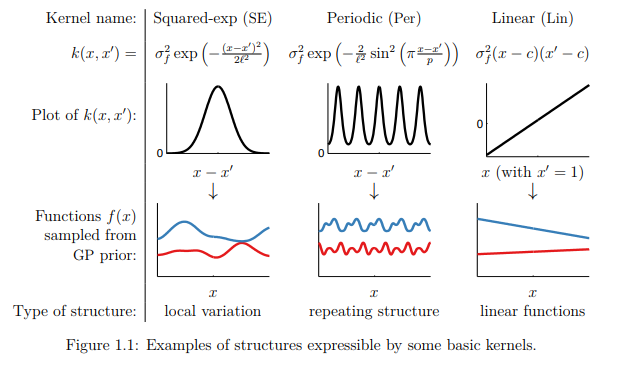
\includegraphics[width=0.7\textwidth]{img/kernels}

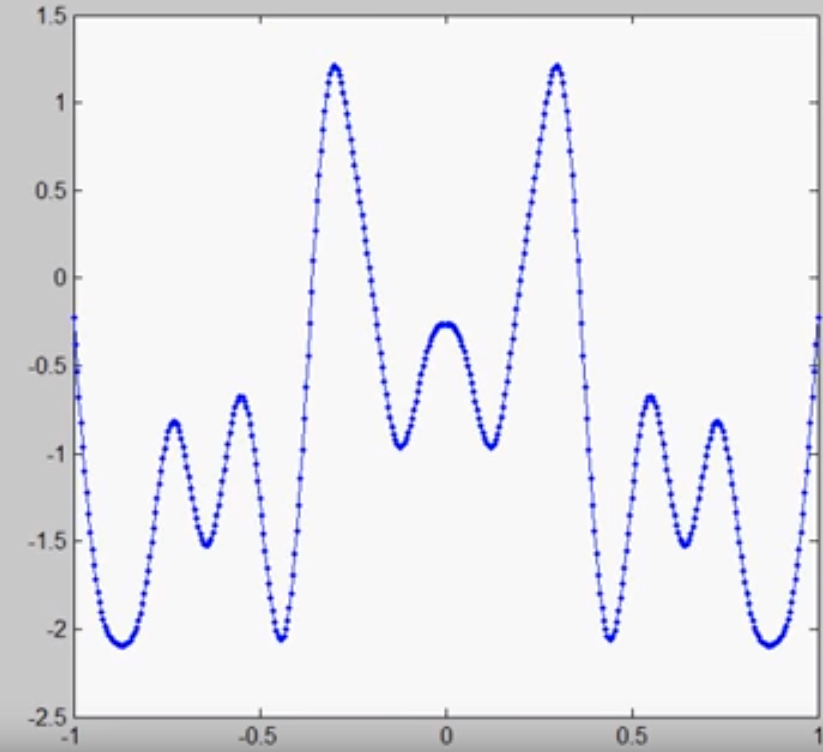
\includegraphics[width=0.7\textwidth]{img/symmetric-kernel}

Image stolen from https://www.cs.toronto.edu/~duvenaud/cookbook/


\begin{tcolorbox}
    \newterm{Gaussian Process} is a \newterm{stochastic process} (a collection of random variables), such that every subset of those random variables has a multivariate Gaussian distribution. It is defined by a mean function $m(x)$ and a covariance funciton $\kappa(x, x')$. Formally, we write \todo{osklive GP}:
    
    \begin{equation}
    f(x) \sim \gN \gG \gP (m(x), \kappa(x, x'))
    \end{equation} \todo{finish}
    
    Bayesian inference ...
    
    \begin{equation}
        \text{posterior} = \frac{\text{likelihood} \times \text{prior}}{\text{evidence}}
    \end{equation},
    
    where evidence is also called \newterm{marginal likelihood}. More concretely, we usually want to compute the posterior distribution over the parameters $\vw$ given the inputs $\mX$ and outputs $\vy$
    
    \begin{equation}
        p(\vw | \vy, \mX) = \frac{p(\vy | \vw, \mX) p(\vw)}{p(\vy | \mX)}
    \end{equation}.
    
    The marginal likelihood is independent of the weights and acts as a normalizing constant. We compute it using marginalization
    
    \begin{equation}
        p(\vy | \mX) = \int p(\vy | \vw, \mX) p(\vw) d \vw.
    \end{equation}
    
    \todo{describe prior over functions}
\end{tcolorbox}


\section{GP from scratch again}



\section{Noise-less Gaussian Process Regression}

\section{Noisy Gaussian Process Regression}


\chapter{TODO Bucket}


\begin{thm}[\citep{murphy2012machine}] (Inverse of a partitioned matrix). Consider a partitioned matrix

\begin{equation}
\mM = \begin{bmatrix} \mA & \mB \\ \mC & \mD \end{bmatrix}
\end{equation}

where we assume $\mA$ and $\mD$ are invertible \todo{staci to? nemusi byt i ty ostatni?}. We have

\begin{equation}
\mM^{-1} = \begin{bmatrix} \mI & \mZero \\ \mI & \mI \end{bmatrix}
\end{equation}
\end{thm}

\begin{proof}
All we need to do is perform a block \newterm{LDU decomposition} and we directly arrive at our solution. We begin by zeroing out $\mB$.

\begin{equation} \label{eq:block-ld-part}
\begin{bmatrix} \mI & -\mB \mD^{-1} & \\ \mZero & \mI \end{bmatrix}
\begin{bmatrix}\mA & \mB \\ \mC & \mD \end{bmatrix} =
\begin{bmatrix} \mA - \mB \mD^{-1} \mC & \mZero \\ \mC & \mD \end{bmatrix}
\end{equation}

The quantity in the top left block is called a \newterm{Schur complement} of $\mM$ wrt $\mD$. We denote it as follows, and also define a variant for the bottom right block

\begin{align}
\mM/\mD &= \mA - \mB \mD^{-1} \mC \\
\mM/\mA &= \mD - \mC \mA^{-1} \mB
\end{align}

Substituting back into \eqref{eq:block-ld-part} we get the following

\begin{equation}
\begin{bmatrix} \mM/\mD & \mZero \\ \mC & \mD \end{bmatrix}
\end{equation}

We follow by eliminating the bottom left block in \eqref{eq:block-ld-part}

\begin{equation} \label{eq:block-du-part}
\begin{bmatrix} \mM/\mD & \mZero \\ \mC & \mD \end{bmatrix}
\begin{bmatrix} \mI & \mZero \\ -\mD^{-1} \mC & \mI \end{bmatrix} =
\begin{bmatrix} \mM/\mD & \mZero \\ \mZero & \mD \end{bmatrix}
\end{equation}

Putting together \eqref{eq:block-ld-part} and \eqref{eq:block-du-part} we get

\begin{equation}
\underbrace{\begin{bmatrix} \mI & -\mB \mD^{-1} & \\ \mZero & \mI \end{bmatrix}}_{\mX}
\underbrace{\begin{bmatrix}\mA & \mB \\ \mC & \mD \end{bmatrix}}_{\mM}
\underbrace{\begin{bmatrix} \mI & \mZero \\ -\mD^{-1} \mC & \mI \end{bmatrix}}_{\mZ} = 
\underbrace{\begin{bmatrix} \mM/\mD & \mZero \\ \mZero & \mD \end{bmatrix}}_{\mW}
\end{equation}

Basic matrix algebra allows us to re-arrange the terms \todo{cite stolen from murphy?}, taking the inverse of both sides

\begin{align}
(\mX \mM \mZ)^{-1} &= \mW^{-1} \\
\mZ^{-1} \mM^{-1} \mX^{-1} &= \mW^{-1} \\
\mM^{-1} &= \mZ \mW^{-1} \mX
\end{align}

Which gives us the final form, making use of the fact that to invert a diagonal matrix we just need to invert its diagonal

\begin{equation} \label{eq:block-inverse}
\mM^{-1} = \begin{bmatrix} \mA & \mB \\ \mC & \mD \end{bmatrix}^{-1} =
\begin{bmatrix} \mI & \mZero \\ -\mD^{-1} \mC & \mI \end{bmatrix}
\begin{bmatrix} (\mM/\mD)^{-1} & \mZero \\ \mZero & \mD^{-1} \end{bmatrix}
\begin{bmatrix} \mI & -\mB \mD^{-1} & \\ \mZero & \mI \end{bmatrix}
\end{equation}

\end{proof}



\section{TODO Linear Gaussian transform - change of variables}

\begin{align}
P(\vx \in \mM) = \int_\mM \frac{1}{(2 \pi)^{D/2} |\mSigma|^{1/2}|} exp \left(-\frac{1}{2} (\vx - \vmu)^T \mSigma^{-1} (\vx - \vmu) \right) d \vx \\
P(\vx \in \mA^{-1} \mM) = \int_{\mA^{-1} \mM} \frac{1}{(2 \pi)^{D/2} |\mSigma|^{1/2}} \exp \left(-\frac{1}{2} (\vu - \vmu)^T \mSigma^{-1} (\vu - \vmu) \right) d \vu \\
\vu = \mA \vx
\end{align}


% \chapter{Bayesian Optimization}

Black box optimization of $f(x)$ where the evaluation is costly. Using GP as a
surrogate model. We use an \newterm{acquisition function} to find where the
next sample should be taken.

\section{Acquisition functions}

In each step, the objective function $f$ is sampled at $x_t = \argmax_x
u(x|D_{1:t-1})$ where $u$ is the acquisition function and $D_{1:t-1} =
((x_1,y_1),\ldots,(x_{t-1},y_{t-1}))$.

\begin{defn}
  \newterm{Expected improvement} $EI(x)$ is defined as

  \begin{equation}
    EI(x) = E_{Y \sim \gN(\mu, \sigma^2)} [max(f(x) - f(x^+), 0)]
  \end{equation}

  where $f(x^+)$ is the value of the best sample so far and $x^+ =
  \argmax_{x_i \in x_{1:t}} f(x_i)$.
\end{defn}

\section{Algorithm}

Iteratively for $t = 1,2,\ldots:$ {TODO NANDO}

\begin{itemize}
  \item Solve $x_t = \argmax_x u(x|D_{1:t-1})$ by combining the attributes of
    the posterior distribution in a utility function $u$.
  \item Sample the objective function $y_t = f(x_t) + \epsilon_t$.
  \item Augment the data $D_{1:t} = \set{D_{1:t-1}, (x_t, y_t)}$ and update
    the GP surrogate model based on the new data.
\end{itemize}


\subsection{Probability of Improvement}

We add a small term $\xi$ because otherwise $PI(x^+) = \frac{1}{2}.$

\begin{align}
  PI(x) &= P(f(x) \geq \mu^+ + \xi) \\
        &= \Phi \left(\frac{\mu(x) - \mu^+ - \xi}{\sigma(x)} \right)
\end{align}

where $\Phi$ is the CDF of a Gaussian. If we knew up front what is the best
value $f(x^*)$ we can model that directly by $P(f(x) \geq f(x^*))$.


\subsection{Expected utility}

At iteration $n+1$, choose the point that minimizes the distance to the
objective evaluated at the maximum $x^*$.

\begin{align}
  x_{n+1} &= \argmin_x E(\norm{ \underbrace{f_{n+1}(x)}_{\text{GP}} - \underbrace{f(x^*)}_{\text{true}\ f} } | D_n) \\
          &=\argmin_x \int \norm{f_{n+1}(x) - f(x^*)} p(f_{n+1} | D_n) \diff f_{n+1}
\end{align}

We however don't know the true objective at the maximum. Instead we use (Mockus
et al., 1978 ??? TODO ref) where $f^{\max} = \mu^+ + \xi$

\begin{equation}
  x = \argmax_x E(\max\set{0, f_{n+1}(x) - f^{max}}|D_n)
\end{equation}

which can be solved analytically with

\begin{align}
  EI(x) &= \begin{cases}
    (\mu(x) - \mu^+ - \xi) \Phi(Z) + \sigma(x)\varphi(Z) & if \sigma(x) > 0 \\
    0 & if \sigma(x) = 0
  \end{cases} \\
  Z &= \frac{\mu(x) - \mu^+ - \xi}{\sigma(x)}
\end{align}

where $\phi(\cdot)$ and $\Phi(\cdot)$ denote the PDF and CDF of a normalized Gaussian.


\subsection{GP-UCB}

Define the \newterm{regret} and \newterm{cumulative regret} as follows:

\begin{align}
  r(x) &= f(x^*) - f(x) \\
  R_T &= r(x_1) + \cdots + r(x_T).
\end{align}

The GP-UCB criterion is as follows:

\begin{align}
  GP-UCB(x) = \mu(x) + \sqrt{\nu \beta} \sigma(x)
\end{align}

with $\nu = 1$ and $\beta_t = 2 \log(t^{d/2 + 2}\pi^2 / 3 \delta)$ where it can
be shown with high probability that this method has no regret, i.e. $\lim_{T
\rightarrow \infty} R_T / T = 0$. (Srinivas et at, 2010 TODO REF). (NOTE, if
the set of points is not infinite, $\beta$ ends up being different).


\subsection{Thompson sampling}

Draw a random sample (function) from the posterior, optimize to find its max,
evaluate the true $f(x)$ at the found max.

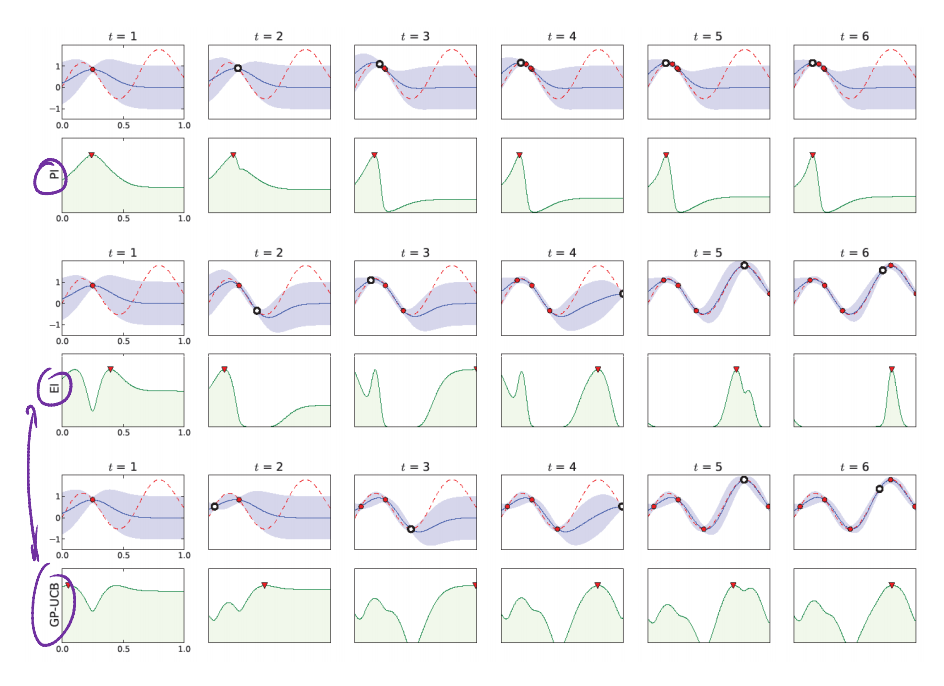
\includegraphics[width=0.9\textwidth]{img/acquisition-functions.png}

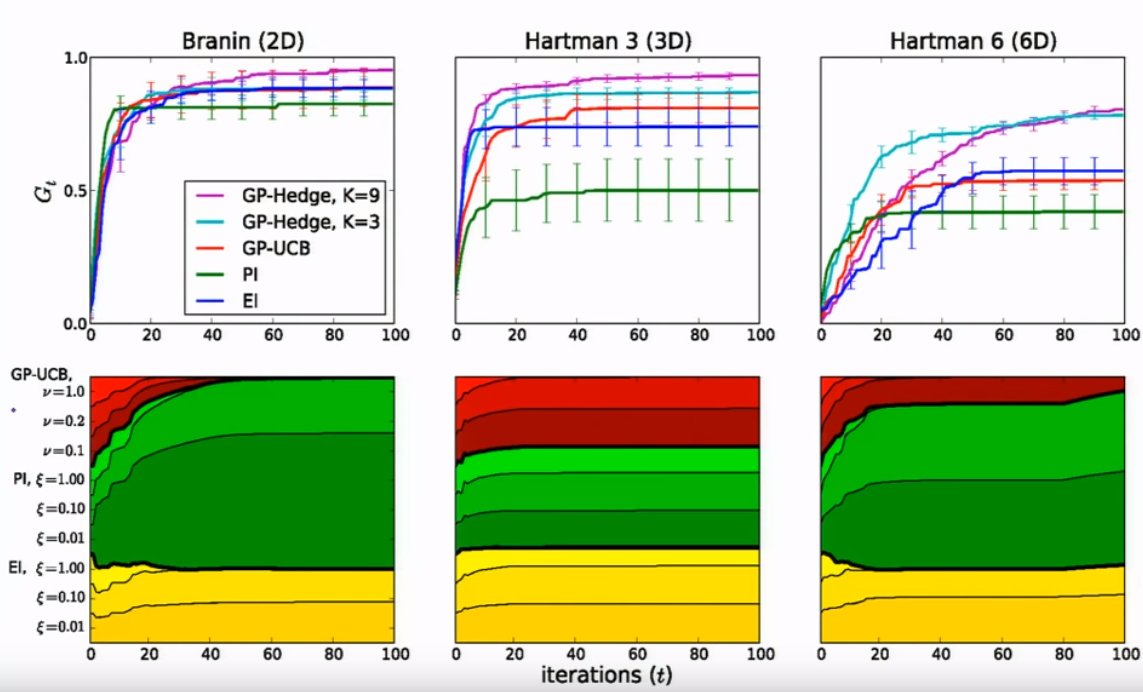
\includegraphics[width=0.9\textwidth]{img/portfolios-of-acquisition-functions.png}


\subsection{Max LCB}

There is no point in sampling where UCB is lower than $\max LCB$ (with high probability).

% \chapter{Appendix?}

\section{Cholesky Decomposition}

\begin{defn}
  The \newterm{Cholesky decomposition} is a decomposition of a
  positive definite matrix into a product of a lower triangular matrix and
  its conjugate transpose. Since we will only work with symmetric
  positive-definite matrices we omit the conjugacy and define Cholesky
  decomposition as

  \begin{equation}
    \mA = \mL \mL^T
  \end{equation}

  where $\mL$ is a lower triangular matrix called the \newterm{Cholesky factor}.
\end{defn}

Because of its numerical stability, Cholesky decomposition is useful for
solving systems of linear equations $\mA \vx = \vb$ where $\mA$ is symmetric
and positive definite. We do this by first solving the triangular system $\mL
\vy = \vb$ by forward substitution, and then the triangular system $\mL^T \vx =
\vy$ by back substitution. This works because

\begin{align}
  \mA \vx &= \vb \qquad \text{assuming $\mA$ is symmetric positive-definite} \\
  \mL\mL^T \vx &= \vb \\
  \mL \vy &= \vb \\
  \mL^T \vx &= \vy \qquad \text{which if we back-substitute $\vy$} \\
  \mL (\mL^T \vx) &= \vy \qquad \text{using associativity} \\
  (\mL \mL^T) \vx &= \mA \vx = \vy.
\end{align}

For brevity, we'll apply the MATLAB {TODO ref} backslash operator where $\mA
\backslash \vb = \vx$, which allows us to write the above as $\vx = \mL^T
\backslash (\mL \backslash b)$.


\section{TODO Bucket}

\begin{thm}[\citep{murphy2012machine}] (Inverse of a partitioned matrix).
  Consider a partitioned matrix

  \begin{equation}
    \mM = \begin{bmatrix} \mA & \mB \\ \mC & \mD \end{bmatrix}
  \end{equation}

  where we assume $\mA$ and $\mD$ are invertible {TODO staci to? nemusi byt i
  ty ostatni?}. We have

  \begin{equation}
    \mM^{-1} = \begin{bmatrix} \mI & \mZero \\ \mI & \mI \end{bmatrix}
  \end{equation}
\end{thm}

\begin{proof}
  All we need to do is perform a block \newterm{LDU decomposition} and we
  directly arrive at our solution. We begin by zeroing out $\mB$.

  \begin{equation} \label{eq:block-ld-part}
    \begin{bmatrix} \mI & -\mB \mD^{-1} & \\ \mZero & \mI \end{bmatrix}
    \begin{bmatrix}\mA & \mB \\ \mC & \mD \end{bmatrix} =
    \begin{bmatrix} \mA - \mB \mD^{-1} \mC & \mZero \\ \mC & \mD \end{bmatrix}
  \end{equation}

  The quantity in the top left block is called a \newterm{Schur complement} of
  $\mM$ wrt $\mD$. We denote it as follows, and also define a variant for the
  bottom right block

  \begin{align}
    \mM/\mD &= \mA - \mB \mD^{-1} \mC \\
    \mM/\mA &= \mD - \mC \mA^{-1} \mB
  \end{align}

  Substituting back into \eqref{eq:block-ld-part} we get the following

  \begin{equation}
    \begin{bmatrix} \mM/\mD & \mZero \\ \mC & \mD \end{bmatrix}
  \end{equation}

  We follow by eliminating the bottom left block in \eqref{eq:block-ld-part}

  \begin{equation} \label{eq:block-du-part}
    \begin{bmatrix} \mM/\mD & \mZero \\ \mC & \mD \end{bmatrix}
    \begin{bmatrix} \mI & \mZero \\ -\mD^{-1} \mC & \mI \end{bmatrix} =
    \begin{bmatrix} \mM/\mD & \mZero \\ \mZero & \mD \end{bmatrix}
  \end{equation}

  Putting together \eqref{eq:block-ld-part} and \eqref{eq:block-du-part} we get

  \begin{equation}
    \underbrace{\begin{bmatrix} \mI & -\mB \mD^{-1} & \\ \mZero & \mI \end{bmatrix}}_{\mX}
    \underbrace{\begin{bmatrix}\mA & \mB \\ \mC & \mD \end{bmatrix}}_{\mM}
    \underbrace{\begin{bmatrix} \mI & \mZero \\ -\mD^{-1} \mC & \mI \end{bmatrix}}_{\mZ} =
    \underbrace{\begin{bmatrix} \mM/\mD & \mZero \\ \mZero & \mD \end{bmatrix}}_{\mW}
  \end{equation}

  Basic matrix algebra allows us to re-arrange the terms {TODO cite stolen from
  murphy?}, taking the inverse of both sides

  \begin{align}
    (\mX \mM \mZ)^{-1} &= \mW^{-1} \\
    \mZ^{-1} \mM^{-1} \mX^{-1} &= \mW^{-1} \\
    \mM^{-1} &= \mZ \mW^{-1} \mX
  \end{align}

  Which gives us the final form, making use of the fact that to invert a
  diagonal matrix we just need to invert its diagonal

  \begin{equation} \label{eq:block-inverse}
    \mM^{-1} = \begin{bmatrix} \mA & \mB \\ \mC & \mD \end{bmatrix}^{-1} =
    \begin{bmatrix} \mI & \mZero \\ -\mD^{-1} \mC & \mI \end{bmatrix}
    \begin{bmatrix} (\mM/\mD)^{-1} & \mZero \\ \mZero & \mD^{-1} \end{bmatrix}
    \begin{bmatrix} \mI & -\mB \mD^{-1} & \\ \mZero & \mI \end{bmatrix}
  \end{equation}

\end{proof}



\section{TODO Linear Gaussian transform}

\todo{change of variables}

\begin{align}
  P(\vx \in \mM) = \int_\mM \frac{1}{(2 \pi)^{D/2} |\mSigma|^{1/2}|} exp \left(-\frac{1}{2} (\vx - \vmu)^T \mSigma^{-1} (\vx - \vmu) \right) d \vx \\
  P(\vx \in \mA^{-1} \mM) = \int_{\mA^{-1} \mM} \frac{1}{(2 \pi)^{D/2} |\mSigma|^{1/2}} \exp \left(-\frac{1}{2} (\vu - \vmu)^T \mSigma^{-1} (\vu - \vmu) \right) d \vu \\
  \vu = \mA \vx
\end{align}

% TODO TODO tohle mozna patri nekam jako summary.
% the parameters are {TODO zkontrolovat kde je $\mu$ a chybi tam vector}
%
% \begin{align}
%   \vmu_{1|2} &= \vmu_1 - \ms{12} \ms{22}^{-1} (\vx_2 - \vmu_2) \\
%   \ms{1|2} &= \mSigma / \ms{22} = \ms{11} - \ms{12} \ms{22}^{-1} \ms{21}
% \end{align}


% TODO: inversion lemma proof vykopirovany jako zaloha
% \begin{proof}
%   All we need to do is perform a block \newterm{LDU decomposition} and we
%   directly arrive at our solution. We begin by zeroing out $\mB$.
%
%   \begin{equation} \label{eq:block-ld-part}
%     \begin{bmatrix} \mI & -\mB \mD^{-1} & \\ \mZero & \mI \end{bmatrix}
%     \begin{bmatrix}\mA & \mB \\ \mC & \mD \end{bmatrix} =
%     \begin{bmatrix} \mA - \mB \mD^{-1} \mC & \mZero \\ \mC & \mD \end{bmatrix}
%   \end{equation}
%
%   The quantity in the top left block is called a \newterm{Schur complement} of
%   $\mM$ wrt $\mD$. We denote it as follows, and also define a variant for the
%   bottom right block
%
%   \begin{align}
%     \mM/\mD &= \mA - \mB \mD^{-1} \mC \\
%     \mM/\mA &= \mD - \mC \mA^{-1} \mB
%   \end{align}
%
%   Substituting back into \eqref{eq:block-ld-part} we get the following
%
%   \begin{equation}
%     \begin{bmatrix} \mM/\mD & \mZero \\ \mC & \mD \end{bmatrix}
%   \end{equation}
%
%   We follow by eliminating the bottom left block in \eqref{eq:block-ld-part}
%
%   \begin{equation} \label{eq:block-du-part}
%     \begin{bmatrix} \mM/\mD & \mZero \\ \mC & \mD \end{bmatrix}
%     \begin{bmatrix} \mI & \mZero \\ -\mD^{-1} \mC & \mI \end{bmatrix} =
%     \begin{bmatrix} \mM/\mD & \mZero \\ \mZero & \mD \end{bmatrix}
%   \end{equation}
%
%   Putting together \eqref{eq:block-ld-part} and \eqref{eq:block-du-part} we get
%
%   \begin{equation}
%     \underbrace{\begin{bmatrix} \mI & -\mB \mD^{-1} & \\ \mZero & \mI \end{bmatrix}}_{\mX}
%     \underbrace{\begin{bmatrix}\mA & \mB \\ \mC & \mD \end{bmatrix}}_{\mM}
%     \underbrace{\begin{bmatrix} \mI & \mZero \\ -\mD^{-1} \mC & \mI \end{bmatrix}}_{\mZ} =
%     \underbrace{\begin{bmatrix} \mM/\mD & \mZero \\ \mZero & \mD \end{bmatrix}}_{\mW}
%   \end{equation}
%
%   Basic matrix algebra allows us to re-arrange the terms {TODO cite stolen from
%   murphy?}, taking the inverse of both sides
%
%   \begin{align}
%     (\mX \mM \mZ)^{-1} &= \mW^{-1} \\
%     \mZ^{-1} \mM^{-1} \mX^{-1} &= \mW^{-1} \\
%     \mM^{-1} &= \mZ \mW^{-1} \mX
%   \end{align}
%
%   Which gives us the final form, making use of the fact that to invert a
%   diagonal matrix we just need to invert its diagonal
%
%   \begin{equation} \label{eq:block-inverse}
%     \mM^{-1} = \begin{bmatrix} \mA & \mB \\ \mC & \mD \end{bmatrix}^{-1} =
%     \begin{bmatrix} \mI & \mZero \\ -\mD^{-1} \mC & \mI \end{bmatrix}
%     \begin{bmatrix} (\mM/\mD)^{-1} & \mZero \\ \mZero & \mD^{-1} \end{bmatrix}
%     \begin{bmatrix} \mI & -\mB \mD^{-1} & \\ \mZero & \mI \end{bmatrix}
%   \end{equation}
%
% \end{proof}


\chapter*{Conclusion}
\addcontentsline{toc}{chapter}{Conclusion}


%%% Bibliography (literature used as a source)
%%%
%%% We employ bibTeX to construct the bibliography. It processes
%%% citations in the text (e.g., the \cite{...} macro) and looks up
%%% relevant entries in the bibliography.bib file.
%%%
%%% The \bibliographystyle command selects, which style will be used
%%% for references from the text. The argument in curly brackets is
%%% the name of the corresponding style file (*.bst). Both styles
%%% mentioned in this template are included in LaTeX distributions.

\bibliographystyle{plainnat}    %% Author (year)
% \bibliographystyle{unsrt}     %% [number]

\renewcommand{\bibname}{Bibliography}

%%% Generate the bibliography. Beware that if you cited no works,
%%% the empty list will be omitted completely.

\bibliography{bibliography}

%%% If case you prefer to write the bibliography manually (without bibTeX),
%%% you can use the following. Please follow the ISO 690 standard and
%%% citation conventions of your field of research.

% \begin{thebibliography}{99}
%
% \bibitem{lamport94}
%   {\sc Lamport,} Leslie.
%   \emph{\LaTeX: A Document Preparation System}.
%   2nd edition.
%   Massachusetts: Addison Wesley, 1994.
%   ISBN 0-201-52983-1.
%
% \end{thebibliography}


%%% Figures used in the thesis (consider if this is needed)
\listoffigures

%%% Tables used in the thesis (consider if this is needed)
%%% In mathematical theses, it could be better to move the list of tables to the beginning of the thesis.
\listoftables

%%% Abbreviations used in the thesis, if any, including their explanation
%%% In mathematical theses, it could be better to move the list of abbreviations to the beginning of the thesis.
\chapwithtoc{List of Abbreviations}

%%% Attachments to the master thesis, if any. Each attachment must be
%%% referred to at least once from the text of the thesis. Attachments
%%% are numbered.
%%%
%%% The printed version should preferably contain attachments, which can be
%%% read (additional tables and charts, supplementary text, examples of
%%% program output, etc.). The electronic version is more suited for attachments
%%% which will likely be used in an electronic form rather than read (program
%%% source code, data files, interactive charts, etc.). Electronic attachments
%%% should be uploaded to SIS and optionally also included in the thesis on a~CD/DVD.
%%% Allowed file formats are specified in provision of the rector no. 72/2017.
\appendix
\chapter{Attachments}

\section{First Attachment}

\printindex

\openright
\end{document}
